\documentclass[12pt]{article}
%
\usepackage{graphicx}
\usepackage[margin=1in,footskip=0.2in]{geometry}%big footskip brings number down, smal
\usepackage{amsmath}
\usepackage{amssymb}
\usepackage[T1]{fontenc}
\usepackage{listings}
\usepackage{bm}
\usepackage{hyperref}
\usepackage{setspace}
\usepackage[usenames]{color}
\usepackage[utf8]{inputenc}
\usepackage{psfrag}
\usepackage[table,xcdraw]{xcolor}
\usepackage{pdflscape}
\usepackage{tikz}
%\usepackage[percent]{overpic}
%\usepackage{wrapfig}
%\usepackage{relsize}
%\usepackage{dsfont}

%
\begin{document}

%
\title{Improving Catch Estimation Methods in Sparsely Sampled Mixed-Stock Fisheries.}
\author{Nick Grunloh$^\text{a}$, Edward Dick$^\text{b}$, Don Pearson$^\text{b}$, John Field$^\text{b}$, Marc Mangel$^\text{a,c}$}
\date{\today}
\maketitle
\noindent
$^\text{a}$ Center for Stock Assessment Research, University of California, Santa Cruz, Mail Stop SOE-2, Santa Cruz, CA 95064, USA.\\
$^\text{b}$ Fisheries Ecology Division, Southwest Fisheries Science Center, National Marine Fisheries Service, National Oceanographic and Atmospheric Administration, 110 McAllister Way, Santa Cruz, CA 95060, USA.\\
$^\text{c}$ Department of Applied Mathematics and Statistics, Jack Baskin School of Engineering, University of California, Santa Cruz, Mail Stop SOE-2, Santa Cruz, CA 95064, USA.

%
%\section{Abstract}\label{abstract}
\begin{abstract}
Effective management of exploited fish populations requires accurate
estimates of commercial fisheries catches to inform monitoring and
assessment efforts. In California, the high degree of heterogeneity in
the species composition of many groundfish fisheries, particularly those
targeting rockfish (genus \(Sebastes\)), leads to challenges in sampling
all potential strata, or species, adequately. Limited resources and
increasingly complex stratification of the sampling system inevitably
leads to gaps in sample data. In the presence of sampling gaps, ad-hoc
species composition point estimation is currently obtained according to
historically derived ``data borrowing'' (imputation) protocols which 
introduce unknown bias and do not allow for uncertainty estimation or 
forecasting. In order to move from the current ad-hoc ``data-borrowing'' point 
estimators, we have constructed Bayesian hierarchical models to estimate 
species compositions, complete with accurate measures of uncertainty, as well 
as theoretically sound out-of-sample predictions. Furthermore, we 
introduce a Bayesian model averaging approach for inferring spatial 
pooling strategies across the over-stratified port sampling system. Our 
modeling approach, along with a computationally robust system of inference 
and model exploration, allows us to 1) objectively compare alternative models 
for estimation of species compositions in landed catch, 2) quantify uncertainty 
in historical landings, and 3) understand the effect of the highly stratified, 
and sparse, sampling system on the kinds of inference possible, 
while simultaneously making the most from the available data.
\end{abstract}

%
\clearpage
\onehalfspacing
%

%
%
\section{Introduction}\label{introduction}
%
%

Estimates of landed catch are a key component of many fishery management
systems. Stock assessment models (referred to here as assessments) are
often conditioned on time series of annual catch, usually under the
assumption that catches are known without error. While some assessment
models are able to incorporate uncertainty in catch (e.g.~Stock
Synthesis; Methot and Wetzel, 2013), reliable estimates of catch
uncertainty are often unavailable. Without this information, assessment
authors often rely on ad-hoc sensitivity analyses which may or may not
be incorporated into management advice and/or fail to propagate catch
uncertainty into quantities of interest to managers.

Over the past decade, the estimation of catch and associated uncertainty
has become a focus for recreational fisheries in the United States (NAS,
2017). Commercial fisheries, on the other hand, are often assumed to
have precise estimates of catch by species. This is due in part to the
availability of landing receipts (aka fish tickets) which serve as a
record of the weight of fish landed into various market categories (sort
groups). As noted by Pearson et al. (2008), it is important to recognize
that species and market categories are not synonymous. On the U.S. West
Coast, for example, it is common for multiple species to be landed
within a single market category (CALCOM 2018, PacFIN 2018). This is
expected for categories that are clearly designated as mixed-species
categories (e.g. ``nearshore rockfish'', or species within a particular
genus or family). However, in some states, categories that are named
after a single species still contain several species, to varying
degrees, even after regulations require sorting into a particular
category (Pearson et al., 2008). As a result, estimation of landings for
a single species based on landing receipt data alone may produce biased
estimates of total catch.

Fisherman, dealers, or processors typically decide how to sort species
into existing market categories (defined by state agencies) on a landing 
receipt. Trained port samplers intercept vessels offloading catch or during 
subsequent processing in order to determine the species composition of catch 
landed in a given market category (Sen 1984, Crone 1995, Tsou et al. 2015). 
These species composition data are used to partition, or distribute, the 
weight of landed catch in a market category across species, a process 
commonly referred to as catch expansion (Pearson and Almany, 1995). To 
estimate total landings for a single species, the expanded catch is summed 
across all relevant market categories. Assuming that landing receipt data 
are a census of the landed catch, uncertainty in total catch for a 
given species reflects variability in the species composition among 
port samples. If information is available to estimate sources of bias in 
the landing receipt data, e.g. underreporting, then it is possible to 
also incorporate uncertainty in the bias correction factors as well 
(Bousquet et al. 2010). In this study, we quantify sampling uncertainty 
for estimates of landed catch, although the modeling framework could be
extended to include uncertainty or bias in landing receipt data.

Within market categories, particularly those used historically for
groupings of highly specious rockfish ($Sebastes$ spp), the species
composition of landed catch can vary spatially, temporally, by fishing
gear, and catch disposition (e.g.~fish sold alive or dead). These
differences are attributable to many factors, including market
preference, fishing behavior, regulatory constraints , and
biological/ecological characteristics (e.g.~spatial distribution) of the
landed species. As a result, estimates of species composition for a
given market category are often stratified over time (e.g.~quarterly)
and across other relevant strata (e.g.~ports, gears, catch disposition
). Sampling programs often have limited funds, and attempts to reduce
bias in species composition estimates through the introduction of
additional strata comes at a cost, namely reduced precision (Cochran,
1977; Tomlinson, 1971).

On the U.S. West Coast, port sampling programs for rockfish and other
groundfish allocate effort both spatially and temporally, but many
domains of interest (e.g.~market category, gear type, catch disposition)
remain unsampled or sparsely sampled due to a proliferation of
categories over time, logistical constraints, and limited resources (Sen
1986; Crone 1995; Pearson et al. 2008; Tsou et al. 2015). In California,
for example, commercial port sampling effort has changed over time and
space (Pearson and Almany 1995). For example, regular sampling of
California ports north of Point Conception (roughly \(34^{\circ}\) 27'
N. latitude) began as early as 1978, but the more southern ports were
rarely sampled prior to 1983. This allocation of effort was largely
based on the statewide distribution of landings, diffuse spatial
distribution of southern commercial ports, and limitations in funding
for port samplers.

When no port samples are collected for landed strata and domains,
species composition estimates are borrowed from other strata using
deterministic algorithms based on expert opinion. These algorithms have
unknown bias and precision. In contrast, model-based estimators are
increasingly used to estimate quantities of interest for domains with
small sample sizes and/or unsampled strata (sometimes referred to as
small area estimation; Rao 2003). As a pilot study, Shelton et al.
(2012) developed a Bayesian hierarchical statistical framework for
estimating species compositions in rockfish market categories from trawl
fisheries from a single port in California in two separate years. Their
model has the ability to partially pool information among sparsely
sampled strata, predicts species compositions for unsampled strata, and
can be combined with landing receipts to estimate total landings by
species, across market categories and other strata, along with
associated estimates of uncertainty. However, their model considered
hierarchical pooling only among quarters within a single year. The
authors also underscored the need to better understand performance of
alternative models, and to overcome issues with computation time,
particularly since commercial port sampling data sets often include
hundreds of landed strata spanning decades, multiple ports, gear types,
and other domains of interest.

Among the U.S. West Coast states, the challenge of estimating landings
for sparsely-sampled mixed stock rockfish fisheries is perhaps greatest
for California. Although overall landings have historically been greater
for rockfish off of Oregon and Washington, California has a greater
number of commercial ports, market categories, and landed species
(Pearson and Irwin 1997). California's commercial landings also have greater 
species diversity among ports due to the geographical range of the coast and 
the observation that species diversity for this genus is greatest in the 
Southern California Bight (Love et al. 2002 ). Lastly, California includes two 
major biogeographic features, Point Conception and Cape Mendocino, that are 
associated with different physical oceanographic conditions and biological 
community assemblages (Hickey 1979, Checkley and Barth 2009, Gottscho 2016), 
and these features are also frequently used as spatial boundaries for 
stock assessments and management measures. Of particular consequence to 
the estimation of species compositions is the proliferation of landed 
market categories over time, particularly during the 1990s, 
Figure (\ref{sparceData})). Sampling effort also leveled off in the mid-1990s, 
with a reduction in effort in the early 2000s, associated with 
substantial declines in total catches as well as reductions in sampling 
resources. The net result of increased stratification and flat (or 
reduced) sampling effort over time is a decline in mean sample size per 
stratum, Figure (\ref{sparceData}). In this situation, it is critical 
to understand how efforts to reduce bias (e.g.~increasing the number of landed 
market categories) affect precision of the expanded catch estimates.

%%%%%%%
Of particular consequence to the estimation of species compositions in 
California is the proliferation of landed market categories over time, 
particularly during the 1990s, see Figure (\ref{sparceData}). Sampling effort 
also leveled off in the mid-1990s, with a reduction in effort in the early 
2000s, associated with substantial declines in total catches as well as 
reductions in sampling resources. The net result of increased stratification 
and flat (or reduced) sampling effort over time is a decline in mean sample 
size per stratum, see Figure (\ref{sparceData}). In this situation, it is 
critical to understand how efforts to reduce bias (e.g. increasing the number 
of landed market categories) affect precision of the expanded catch estimates.
%%%%%%%

Assessments that take catch uncertainty into account are not new (c.f.
Doubleday 1976), but most assessments on the U.S. West Coast assume
catch is known without error (PFMC 2018). As a result, catch uncertainty
is rarely propagated into management reference points. However, the
implications of catch uncertainty are not limited to stock assessment
efforts. In a management context, catch estimates with large (but
unknown) uncertainty may cause managers to react to large,
high-frequency deviations in estimated catch, and either impose
unnecessary restrictions on a fishery, or mistakenly support excessive
harvest. This is particularly an issue for prohibited and/or ``choke''
species, for which catch information is limited and may be based solely on
estimates of discarded catch.

In this study, we evaluate the model-based framework proposed by Shelton
et al. (2012) using commercial port sampling data collected in
California, U.S.A. We describe species composition data collected by the
California Cooperative Groundfish Survey (CCGS, 2017) over the period
1978-1990. We then extend the Shelton et al. framework to address
limitations of their approach. Specifically, we evaluate alternative
likelihoods to address overdispersion, compare multiple hierarchical
structures for pooling information through time, and integrate model
predictions across uncertainties in the spatial model structure.
Finally, we estimate landed catch by species for both sampled and
unsampled strata, and summarize a general framework for quantifying
uncertainty including an efficient database design for dissemination of
results at any level of aggregation.

%
%
\section{Methods}\label{methods}
%
%

\subsection{Data}\label{data}

As outlined in Sen (1984, 1986) the species composition port sampling data
%, held within the CALCOM database, 
are the result of a cluster sampling protocol executed across the many strata 
of California's commercial fisheries.  Each sample is intended to be two fifty-
pound clusters selected at random from a stratum. Although port samplers do 
their best to follow protocol, in reality the port sampling environment does 
not always allow Sen's original protocol to be followed. Variations in the 
sampling protocol may result in only a single cluster being taken, or the size 
of clusters taken to vary from stratum to stratum based on the particular 
challenges of sampling each stratum.

Samples are recorded as integer pounds for each observed species, across the 
landed market categories, gear groups, and port complexes in time (quarters 
within year). Presently there are 71 rockfish market categories, although not 
all market categories are always used. The number of market categories with 
recorded landings has gone from less than 25 in 1978 to about 55 in 2014, see 
Figure (\ref{sparceData}).  Landings are grouped into major fishing gear 
groups (trawl, hook and line, gillnet, fish pot, or other minor categories) 
and ten major port complexes spanning the California coast, see 
Figure (\ref{portMap}).

The model based methodology proposed here does not rely strongly upon
the cluster sampling structure, but rather views each sample as
independent and identically distributed (\(i.i.d.\)) draws from a data
generating model, conditional on a parameterization of the
stratification system. So long as the parameterization and data
generating model are sufficiently robust for handling the behavior of
these data, a conditionally \(i.i.d.\) model of these data will be
practically useful for producing predictions about the data generating
system.

That said, for the purpose of modeling these data, it is enough to know
which clusters were collected as part of which samples, and how big each
cluster actually ended up being. This information is readily available
from CALCOM, a database maintained by the California Cooperative
Groundfish Survey (CALCOM, 2018). Just as in Shelton et al. (2012), we %Specifically
aggregate all observed clusters within each unique sample so that the total 
weight sampled is the sum of pounds in each cluster. Similarly the observed 
weight for a particular species, in each unique sample, is the sum of all of 
the observed weights across clusters.

Although model based data analysis has the potential to add significant
structure to data, a judicious application of these methods must always
confront the model with enough empirical information to adequately learn
about the system. In this setting some market categories and time
periods may not be well enough sampled to learn the parameters of the
models presented here. For this reason, we refrain from modeling any
period where the minimum possible number of effective parameters exceeds
the number of samples for the modeled period. Rather than apply models
inappropriately, these landings are speciated as the nominal species for
their market category. We later demonstrate that due to prioritization
in sampling heavily landed, or otherwise commercially relevant
categories, this sample size heuristic leaves relatively few landings to
be speciated in a statistically uninformed way (i.e. ``nominal''
speciation). Thus nominal speciation represents a negligible component
of the overall expanded landings for most species.

\subsection{Likelihood Modeling}\label{likelihoods}

For the purposes of accurately modeling not only species composition
means, but also higher moments of the data (e.g. variances), it is necessary 
to recognize model limitations with respect to over-dispersed data. Among the 
simplest models for count data are the Poisson and binomial models. Both 
models are typically specified with a single parameter for modeling all of the 
moments of the data, and thus they rely heavily on their respective data 
generating processes to accurately represent higher moments in the data. 
McCullagh and Nelder (1989, pg. 124) commiserate about the prevalence of over-
dispersed data in cluster sampling, and explain ways in which cluster sampling 
itself may result in overdispersion.

Extending the Poisson and binomial models to deal with over-dispersion,
typically involves adding additional parameters for the purpose of
modeling higher moments of the data. The negative binomial (NB)
distribution is often used as an over-dispersed extension of the Poisson
model, since it can be expressly written as an infinite mixture of
Poisson distributions. The beta-binomial model is used as an
over-dispersed extension of the binomial model.

The Poisson and binomial models attempt to model both the mean and
residual variance of the data, with a single parameter for each species.
By definition these models do not have additional parameters to model
the variance, but rather, residual variances in these models are simply
transformations of their mean parameters. Only estimating the mean
parameters in these cases may not be sufficient to produce models which
predict well.

In contrast, the negative binomial and beta-binomial models estimate an
additional parameter which can be used to disentangle the mean and
residual variance estimates. Thus the negative binomial and
beta-binomial models may produce more accurate estimates of the residual
variance, while producing more accurate measures of center. We develop
an example on a subset of data to evaluate statistical support for 
overdisperesed models, see Appendix (\ref{appLike}), which we have 
subsequently used for the purposes of applying at an operational scale.

\subsubsection{Beta-Binomial Model}\label{bbModel}

For a particular market category, \(y_{ijklm\eta}\) is the \(i^{th}\)
sample of the \(j^{th}\) species' weight, in the \(k^{th}\) port, caught
with the \(l^{th}\) gear, in the \(\eta^{th}\) quarter, of year \(m\).
The \(y_{ijklm\eta}\) are modeled as observations from a beta-binomial 
distribution conditional on parameters \(\mu_{jklm\eta}\) and 
\(\sigma^2_{jklm\eta}\),

\[y_{ijklm\eta} \sim BB(\mu_{jklm\eta},~\sigma^2_{jklm\eta}).\]

Above, \(\mu_{jklm\eta}\) is the stratum level mean weight, and
\(\sigma^2_{jklm\eta}\) is the stratum level residual variance.
\(\mu_{jklm\eta}\) is related to a linear predictor,
\(\theta_{jklm\eta}\), via the mean function,

\[\mu_{jklm\eta} = n_{ijklm\eta}\frac{\exp(\theta_{jklm\eta})}{1+\exp(\theta_{jklm\eta})}=n~\text{expit}(\theta_{jklm\eta})=n~\text{logit}^{-1}(\theta_{jklm\eta}).\]

Here \(n_{ijklm\eta}\) is the observed aggregate cluster size for each
sample. Additionally, \(\sigma^2_{jklm\eta}\) is related to
\(\mu_{jklm\eta}\) and the overdispersion parameter, \(\rho\), via the
following equation,

\[\sigma^2_{jklm\eta} = \mu_{jklm\eta}\Big(1-\frac{\mu_{jklm\eta}}{n_{ijklm\eta}}\Big)\Big(1+(n_{ijklm\eta}-1)~\rho\Big).\]

\(\rho\) is the within-cluster correlation. The situation where
\(\rho\rightarrow1\) represents identical information content among
replicates within a cluster, with maximal overdispersion relative to the
binomial distribution. The situation where \(\rho\rightarrow0\)
represents totally independent information content among replicates
within a cluster, and the beta-binomial model approaches the binomial
model. \(\rho\) explicitly models average overdispersion across all
strata within a market category, while \(\mu_{jklm\eta}\) gives the
model flexibility at the stratum level through the \(\theta\) linear
predictors,

\[\theta_{jklm\eta} = \beta_0 + \beta^{(s)}_j + \beta^{(p)}_k + \beta^{(g)}_l + \beta^{(t)}_{m\eta}.\]

Firstly, \(\theta\) includes a reference level intercept (\(\beta_0\)).
Secondly, \(\theta\) is factored among the many strata by additive
offsets from \(\beta_0\) for each of the species (\(\beta^{(s)}_j\)),
port-complexes (\(\beta^{(p)}_k\)), and gear-groups (\(\beta^{(g)}_l\)).
Finally year and quarter parameters are indicated generally here inside
the \(\beta^{(t)}_{m\eta}\) term. Several forms for
\(\beta^{(t)}_{m\eta}\) are explored each implying a different prior and
partial pooling strategies as described in the following
section(\(Priors\)).

\subsection{Priors}\label{priors}

To complete the Bayesian formulation of this model, priors are expressed
in a largely diffuse manner.

\[\beta_0 \propto 1\]
\[\left\{\beta^{(s)}_j, \beta^{(p)}_k, \beta^{(g)}_l\right\} \sim N(0, 32^2)\]

Since the \(\beta_0\) reference level is chosen arbitrarily, with no
conception of which values it may take, no restrictions are placed on
the value of the intercept. The species (\(\beta^{(s)}_j\)),
port-complex (\(\beta^{(p)}_k\)), and gear-group (\(\beta^{(g)}_l\))
offsets are assigned diffuse normal priors. The large fixed values of
the prior variance hyperparameters produce behavior similar to classical
fixed effect models for species, port-complex, and gear- group
parameters.

In returning to the time parameter model, \(\beta^{(t)}_{m\eta}\), it is
useful to consider how overparameterized models may cause overfitting
and weaken model performance through the bias-variance dilemma
(Ramasubramanian, K., \& Singh, A., 2016). Simply put, the bias-variance
dilemma means that model formulation is not simply a bias reduction
task, but rather the goal is to formulate models which reduce bias,
while jointly minimizing uncertainty. Janyes (2003, pg. 511) describes
how the inclusion of estimation bias via the Bayesian methodology may
produce better performing estimates, more quickly, than unbiased
counterparts. Among the simplest ways to see the principle is in the
structure of the MSE performance metric, and how it can be explicitly
written to value both estimator bias and variance, as follows.

\[\text{MSE}(\hat\theta) = \mathbb{E}\left[~(\hat\theta - \theta)^2~\right] = \overbrace{\mathbb{E}\Big[~\left(\hat\theta-\mathbb{E}(\hat\theta)\right)^2~\Big]}^{\text{Var}(\hat \theta)} + \overbrace{\Big(~\mathbb{E}(\hat\theta)-\theta~\Big)^2}^{\text{Bias}(\hat \theta, \theta)^2}\]

Furthermore a model can minimize bias, without regard for estimation
uncertainty, by including one model parameter to be fit to each
observation. These parameter estimates are totally unbiased, however
such a model is also predictively useless since each estimated parameter
is specifically bound to a\\
particular observation, and thus such a model does not generalize.

For modeling \(\beta^{(t)}_{m\eta}\) we consider a spectrum of models
which span a wide range of partially pooled models with several
different predictive structures as seen below.

\subsubsection{(M1)}\label{m1}

\[\beta^{(t)}_{m\eta} = \beta^{(y)}_{m} + \beta^{(q)}_{\eta}\]
\[\beta^{(y)}_{m} \sim N(0, 32^2)\]
\[\beta^{(q)}_{\eta} \sim N(0, 32^2)\]

(M1) represents a fixed effects model for additive year and quarter
parameters. Here each year and quarter are assigned totally independent
and diffuse priors.

\subsubsection{(M2)}\label{m2}

\[\beta^{(t)}_{m\eta} = \beta^{(y)}_{m} + \beta^{(q)}_{\eta}\]
\[\beta^{(y)}_{m} \sim N(0, v^{(y)})\]
\[\beta^{(q)}_{\eta} \sim N(0, v^{(q)})\]

(M2) estimates two hierarchical variance parameters, \(v^{(y)}\) and
\(v^{(q)}\). \(v^{(y)}\) has the effect of partially pooling information
among year parameters, while \(v^{(q)}\) partially pools information
among quarter parameters (i.e. treats both year and quarter as ``random
effects''). The actual degree of pooling among each of the years and
quarters is determined by the data.\\
Depending on the posterior distributions of \(v^{(y)}\) and \(v^{(q)}\),
the \(\beta^{(y)}\) and \(\beta^{(q)}\) may be shrunk back toward the
common mean (for small \(v\)) or allowed to take largely distinct values
(in the case of large estimates of the \(v\)).

\subsubsection{(M3)}\label{m3}

\[\beta^{(t)}_{m\eta} = \beta^{(y)}_{m} + \beta^{(q)}_{\eta} + \beta^{(y:q)}_{m\eta}\]
\[\beta^{(y)}_{m} \sim N(0, v^{(y)})\]
\[\beta^{(q)}_{\eta} \sim N(0, v^{(q)})\]
\[\beta^{(y:q)}_{m\eta} \sim N(0, v)\]

(M3) functions similarly as (M2), in that it has hierarchical partial
pooling among both the \(\beta^{(y)}_{m}\) and \(\beta^{(q)}_{\eta}\)
parameters, except that it introduces a two-way interaction term between
year and quarter. This interaction term allows estimates for particular
quarters to differ from year to year, as opposed to the previous models
in which quarters within a year are assumed to be identical from year to
year.

Furthermore the \(\beta^{(y:q)}_{m\eta}\) are also modeled
hierarchically to introduce a single variance parameter, \(v\), shared
among all of the \(m\eta\) time chunks. Although this interaction term
adds many parameters to the model, the shared \(v\) parameter functions
to shrink extraneous \(\beta^{(y:q)}_{m\eta}\) estimates back toward the
common stratum mean.

\subsubsection{(M4)}\label{m4}

\[\beta^{(t)}_{m\eta} = \beta^{(y:q)}_{m\eta}\]
\[\beta^{(y:q)}_{m\eta} \sim N(0, v)\]

(M4) simplifies (M3) by excluding year and quarter main effects. This
leaves all temporal information in the data to be modeled solely by the
quarterly \(\beta^{(y:q)}_{m\eta}\) interaction terms. This model
represents more opportunity for partial pooling through time than (M3),
as fewer time parameters are introduced. Furthermore all of the
\(\beta^{(y:q)}_{m\eta}\) are hierarchically pooled back toward a single
common stratum mean via the single shared variance parameter, \(v\). 

A model treating the interaction terms as fixed effects (e.g. model (M4) where 
$v$ is a large fixed value) was not considered. The \(\beta^{(y:q)}_{m\eta}\) 
interaction terms introduce a very large number of parameters, which require 
regularization in this setting. Furthermore, pooling \(\beta^{(y:q)}_{m\eta}\) 
through time introduces a formalized way to make predictions about unsampled 
strata.

% with fixed \(\beta^{(y:q)}_{m\eta}\) interaction terms are
%considered here, as these models introduce a very large number of
%parameters. Due to the sparsity of these data, the models ability to
%pool through time is important for allowing model flexibility in time,
%while retaining the ability to produce predictions for unsampled time
%periods.

\subsubsection{(M5)}\label{m5}

\[\beta^{(t)}_{m\eta} = \beta^{(y:q)}_{m\eta}\]
\[\beta^{(y:q)}_{m\eta} \sim N(0, v_\eta)\]

(M5) is largely the same as (M4), but it represents slightly less
potential partial pooling through its hierarchical prior variances,
\(v_\eta\), on \(\beta^{(y:q)}_{m\eta}\). Here interaction terms are
allowed to partially pool interactions across years, within a common
quarter, but since each quarter is assigned a separate variance
parameter no pooling is possible between quarters.

\subsubsection{(M6)}\label{m6}

\[\beta^{(t)}_{m\eta} = \beta^{(y:q)}_{m\eta}\]
\[\beta^{(y:q)}_{m\eta} \sim N(0, v_m)\]

(M6) follows the same idea as (M5), however here interaction terms are
allowed to partially pool interactions within a common year, across the
quarters of that year, but not between years. (M6) often involves
fitting slightly more parameters than (M5) because, at least in this
setting, it is typical to model more than four years of data at once.

Historically, regulations have been enacted with the aim of isolating
catch in a market category to a single species (sort requirements). This
clearly affects the composition of the target market category, but these
regulations also affect the species composition of other market
categories in which the target species previously occurred. We
incorporate this information into the model structure by treating time
periods with relatively stable regulatory conditions as independent
models. In other words, information is only shared among years in which
regulations were similar. For example, a sort requirement for widow
rockfish ($S. entomelas$) was initiated in 1983. This not only affected
the composition of the widow rockfish market category (269), but also
the composition of other categories, such as the unspecified rockfish
market category (250). We model the first five years of available data
(1978-1982) independently from the years 1983-1990. In 1991, a sort
requirement for bocaccio rockfish ($S. paucispinis$) was enacted, which is
known to have affected the composition of other categories, including the 
Chilipepper rockfish market category (254) and the Chilipepper/Bocaccio market 
category (956).

Hierarchical variance parameters are estimated from the data. As the
above models learn the posteriors of the hierarchical variance
parameters, it affects the degree of shrinkage as well as the effective
number of parameters held within the respective hierarchies (Gelman,
2014). To achieve this, each variance parameter must itself be assigned
a prior to be estimated. For all of the hierarchical variance parameters
included in the above models \(v\) is assigned a diffuse inverse gamma
(IG) prior \(v \sim IG(1,~2\times10^{3})\).

Finally the overdispersion parameter, \(\rho\), is assigned a diffuse
normal prior on the logit scale, \(\text{logit}(\rho) \sim N(0, 2^2)\).
The \(N(0, 2^2)\) prior is indeed a symmetric, and far reaching, prior
when back transformed to the unit interval. To notice this, it is
helpful to realize that the central 95\% interval for a \(N(0, 2^2)\)
(i.e. \(0\pm3.91\)), includes almost the entirety of the back
transformed unit interval (i.e. \(0.5\pm0.48\)).

For the purpose of motivating the time parameter structure to be used across 
all market categories and time periods, each of models M1-M6 are fit to data 
from market category 250 from 1978-1982. % in order to motivate the time parameter structure to be used across all market categories and time periods. 
Performing such a model selection exercise across all market categories, in 
each time period, would not only be impractical but would also risk overfitting 
models, particually in poorly sampled categories. In the early time periods, 
market category 250 is the most heavily sampled multi-species market category, 
and thus it represents an excellent data-set for testing.

% in the best sampled 
%market category 250, with Table(\ref{priorTab}) guiding the use of model (M4) for the
%duration of the study.

\subsection{Species Composition Prediction}\label{species-composition-prediction}

Bayesian inference of the above models gives access to the full
posterior distribution of all of the parameters of the model given the
data. It is useful to emphasize that in the Bayesian setting, these
parameters have full distributions, and they are typically handled as a
large number of samples from the joint posterior distribution of the
parameters. Once the posterior sampling is complete, this simplifies
parameter mean and variance estimation; required moments are simply
obtained by computing the desired moments from the posterior samples.
Additionally, the fact that the parameters are full distributions means
that any functions of those parameters are themselves random variables
with the function representing a transformation of those parameters.

To obtain predicted species compositions from the beta-binomial model, first 
consider the posterior predictive distribution of sampled weight for a 
particular stratum.

\[p(y^*_{jklm\eta}|y) = \int\!\!\!\!\int\! \text{BB}\Big( y^*_{jklm\eta}|\mu_{jklm\eta}, \sigma^2_{jklm\eta} \Big) P\Big(\mu_{jklm\eta}, \sigma^2_{jklm\eta} | y\Big) d\mu_{jklm\eta} d\sigma^2_{jklm\eta}.\]

Here BB is the data generating beta-binomial distribution for a
predictive observation and \(P(\mu_{jklm\eta}, \sigma^2_{jklm\eta}|y)\)
is the posterior distribution of the parameters given the observed data.
\(\mu_{jklm\eta}\) and \(\sigma^2_{jklm\eta}\) are integrated numerically via 
Monte Carlo integration to produce samples from the predictive distribution, 
\(p(y^*_{jklm\eta}|y)\), for sampled weights in the \(jklm\eta^{th}\) stratum.

Obtaining predictive species compositions from predictive weights
amounts to computing the following transformation,

\[\pi^*_{jklm\eta} = \frac{y^*_{jklm\eta}}{\sum_j y^*_{jklm\eta}} ~~~ y^*_{klm\eta}\neq 0.\]

For a particular market category, \(\pi^*_{jklm\eta}\) is predicted
proportion of species \(j\) in the \(k^{th}\) port, caught with the
\(l^{th}\) gear, in the \(\eta^{th}\) quarter, of year \(m\).

\subsection{Expansion of Landed Catch to Species}\label{expansion}

For a particular market category, speciated landings simply amounts to
the multiplication of the known total landings (\(\lambda_{klm\eta}\)),
reported on landing receipts in the \(klm\eta^{th}\) stratum, with the
posterior predictive species composition, \(\pi^*_{jklm\eta}\), as follows

\[\lambda^*_{jklm\eta} = \lambda_{klm\eta}\pi^*_{jklm\eta}.\]

\(\lambda^*_{jklm\eta}\) is then the posterior predictive landings for
species \(j\) in the \(klm\eta^{th}\) stratum of a particular market
category. Recall that since \(\pi^*_{jklm\eta}\) is a random variable,
then so is \(\lambda^*_{jklm\eta}\). Computing the variance of
\(\lambda^*_{jklm\eta}\) simply amounts to computing the variance of
random draws from the \(\lambda^*_{jklm\eta}\) distribution.
Furthermore, any level of aggregation of \(\lambda^*_{jklm\eta}\) is
easily obtained by summing \(\lambda^*_{jklm\eta}\) draws across the
desired indices. For example to obtain the distributions of yearly catch
of Bocaccio in a particular market category, i.e. aggregated across ports, 
gears, and quarters, one simply fixes $j$ to Bocaccio, and computes the 
following transformation of \(\lambda^*_{jklm\eta}\),

\[\lambda^*_{j\cdot\cdot m\cdot} =\sum_{k}\sum_{l}\sum_{\eta}\lambda^*_{jklm\eta}\].

Distribution summaries such as quantiles, means, or variances may be
computed by computing those metrics from the random draws of the
resulting \(\lambda^*_{j\cdot\cdot m\cdot}\) distributions.

\subsection{Model Exploration \& Averaging}\label{model-exploration-averaging}

Presently, strata with diminishingly small sample sizes are managed by
an ad-hoc ``data borrowing'' protocol, as outlined in Pearson and Erwin
(1997). The protocol for ``data borrowing'' calls for pooling only when
forced to fill holes brought about by unsampled strata. Naturally, such
a pooling protocol introduces bias to fill in unsampled strata, however
due to the mathematically unstructured way in which this bias is
introduced, it is hard to quantitatively justify these ``data
borrowing'' rules.

Model (M4) avoids temporal ad-hoc ``borrowing'' protocols described in
Pearson and Erwin (1997) by making use of its hierarchical structure to
fill temporal holes with a posterior predictive distribution for unseen
time periods within the modeled period. This hierarchical structure uses
the data to estimate the degree of pooling through time, rather than
ad-hoc ``data borrowing''. In addition, the M4 model allows data collected 
during periods with similar regulations to inform predictions across both 
quarters and years, unlike the previous ad-hoc approach which only shared 
information among quarters within a year.

Despite the benefits of modeling these data as Bayesian hierarchical
models, port sampling data still remains sparse. Given the degree of
sparsity in these data it is certainly possible that models which
consider an additional degree of data pooling between port complexes may
offer predictive benefits. In exploring strategies for pooling data
across space it is necessary to formalize the port complex pooling
scheme in a way which provides a mathematically understandable and
scalable structure to build upon.

Given the spatial structure, and complex behavior of, port complex
parameters, the typical zero mean hierarchical regularization priors are
not appropriate among port complexes. Pooling across spatial categorical
parameters in this setting requires the ability to pool port complex
parameters back toward an unknown number (\(\le K\)) of mean levels.
Rather than hierarchically regularize port complex, we frame port
complex pooling as a model uncertainty problem, in which we consider
some degree of full pooling among port complex, but the exact degree of
pooling, and the particular partitioning of the pooled port complexes
are not known.

Port complex pooling is achieved by repeatedly fitting model (M4) with
different partitionings of the port complex variables within a
particular market category and modeling time period. This model
exploration exercise explores the possible ways to produce groupings of
the existing port complexes so as to discover predictively useful
partitionings of the port complexes. Insisting that the port complex
groupings be partitions of the available port complexes provides a
well-defined mathematical structure for exploring the space of pooled
port complexes.

The size of the space of possible pooled models is in the setting is
well defined in terms of the size of the set of items to be partitioned,
\(K\), as given by the Bell numbers (\(B_K\)),

\[B_K=\sum_{\hat k=0}^{K} \frac{1}{\hat k!} \left( \sum_{j=0}^{\hat k} (-1)^{\hat k -j} \left(\substack{\hat k \\ j}\right) j^K \right).\]

In the case of California the set of items to be partitioned is the set
of port complexes in California, of which there are \(K=10\), implying a
grand total of \(B_{10}=115975\) ways of partitioning the port complexes
in California in each market category and modeled time period. The brute
force model selection strategy of computing all 115975 of these
partitionings strategies is computationally infeasible. However, not all
pooling schemes represent biologically relevant models. For example, it
is likely reasonable to pool only among adjacent ports (i.e.~no
discontinuities between port complex pooling in space) due to species
distributions and the presence of biogeographical provinces, and it may
be similarly reasonable to assert that similar regions can only extend
across a small number of ports.

We limit the set of models to be considered by applying two constraints. 
1) Only adjacent port poolings are considered, and 2) the maximum size of a 
port complex grouping is fixed to be no larger than three port complexes. 
These two constraints were chosen so as to mirror the currently accepted 
protocols in Pearson and Erwin (1997), although many other constraints may, in 
theory, be chosen.
%constraints were chosen so as to mirror the currently accepted protocols
%in Pearson and Erwin (1997) within the context of this framework. 
When these two simple constraints are applied, the number of models to
explore in each modeled period is reduced to a much more manageable 274
models. It this framework, it is not necessary to impose a priori conditions 
on how data are shared among ports (e.g. never borrowing across Point 
Conception, as in the current ad hoc approach). However, if the data strongly 
support a particular port configuration, models with that structure will have 
greater influence on model predictions.

An exhaustive search of the models in the constrained subspace of
\(B_{10}\), allows for a concrete comparison of the relative predictive
accuracy of each partitioning. Additionally the partitioned models
provide a set of candidate models for use in Bayesian Model Averaging
(BMA) (Hoeting et al., 1999). BMA, as applied here, allows the model
exploration strategy to average models across all potentially relevant
partitions of the port complexes, so as to add robustness to final
species composition estimates.

For the \(\iota^{th}\) model in a set of candidate models \(M\), then
the BMA weight for \(M_\iota\) follows directly from Bayes Theorem as,

\[\omega_\iota = Pr(M_\iota|y) = \frac{ p(y|M_\iota)p(M_\iota) }{ \sum_\iota p(y|M_\iota)p(M_\iota) }.\]

Where \(\omega_\iota\) is the posterior probability that model \(\iota\)
is the true data generating model of the data, conditional on the
subspace of candidate models and the observed data. \(\omega_\iota\) is
then straightforwardly used to average posteriors across all of the
models, as

\[\bar p(\theta|y) = \sum_{\iota} \omega_\iota p(\theta|y, M_\iota).\]

[EJ to insert methods subsection here on landings by species-year-gear, as 
well as comparison to CALCOM]

%
%
\section{Results}\label{results}
%
%

\subsection{Characteristics of the Landings Data}\label{landData}

In the two time periods modeled here, Figures (\ref{bar78} and \ref{bar83}) 
show how commercial port sampling effort tracks both total landed weight as
well as the number of species in market categories accounting for the
top 99\% of total landings in each time period. Comparable results for
the periods 1991-1999 and 2000-2015 are discussed Appendix (\ref{appData}), 
although we have not yet completed modeling for these time periods. 
Our model is applied to a relatively large proportion of the landings in both 
time periods, and nominal speciation occurs for a relatively negligible 
proportion of total landings. %It is important to notice that since 
This is because 1)port sampling effort is largely opportunistic and implicitly 
prioritizes heavily landed market categories, and 2) our model is only fit to 
market categories with more data than model parameters. As a result market 
categories left with too few samples to fit our model tend to be less landed. 
%Thus our model is applied to a relatively large proportion of the landings and nominal 
%speciation occurs for a relatively negligible proportion of total landings. 
Applying the sample size heuristic to determine which market categories are 
expended by our model results in 96.8\% of landed weight being expanded via 
our model in the 1978-1982 time and 98.3\% of landed weight expanded by our 
model in 1983-1990.

The lower panels of Figures (\ref{bar78} and \ref{bar83}) demonstrate just how
many different species are landed into commercially relevant market
categories. Although market categories often carry names that label them
with a nominal species, Figure (\ref{bar78}) makes it abundantly clear that
these names can mislead our thinking about the purity, and consistency,
of these categories through time. To drive this point, consider the
sampled species in market category 267 in 1978-1982. The nominal label
for market category 267 is Brown Rockfish, while Brown Rockfish only
amounts to a small fraction of that category in 1978-1982. In fact, only
6.3\% of the sampled weight in 1978-1982 consisted of Brown Rockfish. In
1978-1982 market category 267 might be better named Widow Rockfish as
Widow amounts to 92.6\% of sampled weight in this time period, however
market category 267 is composed of 99.6\% Brown and 0\% Widow in recent
time periods (see Appendix \ref{appData}).

\subsection{Predictor and Prior Selection}\label{predictor-and-prior-selection}

\begin{table}[h!]
\centering
\begin{tabular}[c]{@{}lcccccc@{}}
%\toprule
\hline
& M1 & M2 & M3 & M4 & M5 & M6 \\ \hline
%\midrule
%\endhead
MSE & 0.127245 & 0.127042 & 0.126801 & 0.122373 & 0.127236 & 0.126573 \\ %\hline
\(\Delta\) DIC & 2558.56 & 2259.94 & 2013.21 & 0 & 2175.32 & 2174.71 \\ %\hline
\(\Delta\) WAIC & 2562.65 & 2263.58 & 2009.32 & 0 & 2171.18 & 2170.56 \\ %\hline
\(pr(M|y)\) & \(\approx0\) & \(\approx0\) & \(\approx0\) & \(\approx1\) & \(\approx0\) & \(\approx0\) \\ \hline
%\bottomrule
\end{tabular}
\caption{A table showing Mean Squared Error (MSE; computed on the species
composition scale), delta deviance information criterion (\(\Delta\) DIC),
delta widely applicable information criterion (\(\Delta\) WAIC), and marginal
Bayesian model probabilities (\(pr(M|y)\)) across the fit of models M1-M6 to 
data from 1978-1982 in market category 250.}
\label{priorTab}
\end{table}

%Table (\ref{priorTab}) displays the result of fitting models (M1)-(M6) to data
%from 1978-1982 in market category 250. 
Recall models (M1)-(M6) differ in the structure of the \(\beta^{(t)}_{m\eta}\) 
time parameters. Table (\ref{priorTab}) shows the relative support for those 
model structures. From (M1) to (M4) the models represent a spectrum of models 
with an increasing potential of shrinkage among time parameters. Models 
M5 and M6 represent models which build in complexity, from (M4), via 
the inclusion of multiple hierarchical variance parameters among 
the interaction terms.

Across all of the time models, model M4 displays consistent support over
all other candidate models considered here. It is worth mentioning that
among all of the models considered here, (M4) offers the largest
potential for hierarchical partial pooling among the time parameters.
Model (M4) represents a model with maximal potential for pooling through
time, while still maintain the ability to model differences in
seasonality from year to year.

\subsection{Model Exploration \& Averaging}\label{model-exploration-averaging-1}

%\begin{figure}[h!]
%\centering
%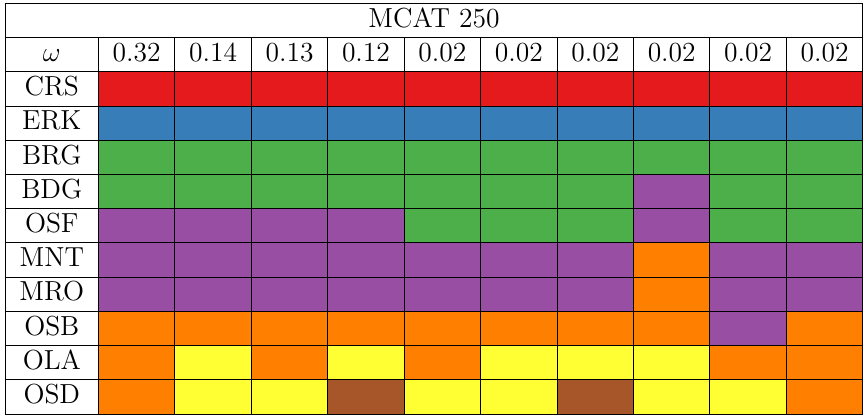
\includegraphics{./pictures/tinyTrim.png}
%\caption{model selection: 1978 to 1982}
%\label{colorTab78}
%\end{figure}

%Figure (\ref{colorTab78}) shows the results of port complex model
%selection for the modeled period from 1978 to 1982 in market category
%250. Along the top BMA weights (\(\omega\)) for the top 10 models are
%displayed (each column is a distinct model). The following ten rows
%indicate the ten port complexes in California, and the colored cells
%indicate how port complexes are partitioned in each model.

Considering Figure (\ref{colorTab78}), the best partitioned model
(first column, \(\omega=0.32\)) gives distinct parameters to CRS and
ERK, while pooling BRG/BDG, OSF/MNT/MRO, and OSB/OLA/OSD. This model
uses five parameters to model the ten ports complexes in California.
Given the set of candidate models explained above, the BMA procedure
gives this model a probability of 32\%. Notice that the only difference among 
the top four models is in how the port complexes south of Point Conception are 
handled. In fact, the seven northerly port complexes are identically 
partitioned in the top four models, which also represent all of the possible 
partitionings of the southern three port complexes.

In this modeled period it is known that no species composition sampling
was done south of Point Conception, thus it is not surprising that these
models perform similarly. When no data are present, parameters simply
represent place holders for out of sample prediction. Since the port
complexes south of Point Conception are not informed by data, the
predictions are identical in these categories. Since the first model
makes identical predictions to the following three, and does so using
the fewest parameters, it is correctly identified as the most
parsimonious explanation among these data.

Considering how the top four model configurations share identical
structure in the seven northerly port complexes, while exhaustively
spanning the candidate partitions south of Point Conception, it is
simple to see that BMA assign's approximately 71\% marginal probability
to the northerly model structure.

The results shown here only represent a single market category across
the time period 1978-1982. Similar results for other market categories
and time periods are provided in Appendix (\ref{appBMA}).

\subsection{Prediction}\label{prediction}

Repeatedly fitting model (M4) across port complex configurations and
applying the BMA procedure, ultimately provides access to posterior
predictive distributions of the species compositions
(\(\pi^*_{jklm\eta}\)) within a market category and time interval
modeled period. A straight forward way to evaluate the performance of
the model in each modeled period is to compare the predictions of the
model in each modeled period with the actual observations of species
compositions from port samplers.

We evaluate species composition posterior predictive distributions via
HDI at three levels containing 68\%, 95\%, and 99\% of posterior
predictive probability. Tables (\ref{predTab78} and \ref{predTab83}) 
show the proportion of observed species compositions which existed within the 
HDI across all strata, of each prediction level, in each modeled period. For 
example, observed species compositions for market category 250 in the 
1978-1982 time period fell within the 68\% HDI of the posterior 
predictive distribution 67.1\% of the time, Table (\ref{predTab78})).

%\subsubsection{78-82}\label{section}
\begin{table}[h!]
\centering
\begin{tabular}[c]{@{}llll@{}}
%\toprule
\hline
& 68\% & 95\% & 99\% \\ \hline
%\midrule
%\endhead
250 & 67.1\% & 96.1\% & 98.7\% \\
253 & 67.3\% & 96.3\% & 98.9\% \\ 
262 & 67.4\% & 93.8\% & 95.3\% \\
265 & 69.6\% & 96.0\% & 97.8\% \\
269 & 68.2\% & 88.8\% & 90.2\% \\
270 & 68.6\% & 93.6\% & 96.7\% \\
956 & 68.3\% & 96.7\% & 99.2\% \\
959 & 68.5\% & 96.3\% & 98.1\% \\
961 & 69.3\% & 93.2\% & 95.3\% \\
AVG & 68.3\% & 94.5\% & 96.7\% \\ \hline
%\bottomrule
\end{tabular}
\caption{1978-1982}
\label{predTab78}
\end{table}

%\subsubsection{83-90}\label{section-1}
\begin{table}[h!]
\centering
\begin{tabular}[c]{@{}llll@{}}
%\toprule
\hline
& 68\% & 95\% & 99\% \\ \hline
%\midrule
%\endhead
245 & 60.8\% & 94.9\% & 97.7\% \\  
250 & 68.1\% & 96.0\% & 99.0\% \\
253 & 69.3\% & 97.1\% & 98.9\% \\
259 & 83.8\% & 91.9\% & 92.9\% \\
262 & 68.5\% & 95.1\% & 95.9\% \\
269 & 68.6\% & 94.2\% & 94.7\% \\
270 & 67.9\% & 94.2\% & 96.7\% \\
663 & 68.1\% & 94.1\% & 96.3\% \\
667 & 69.4\% & 92.5\% & 93.5\% \\
956 & 67.5\% & 96.2\% & 99.0\% \\
959 & 67.4\% & 96.4\% & 99.0\% \\
960 & 68.0\% & 96.1\% & 98.6\% \\
961 & 68.6\% & 94.6\% & 97.8\% \\
AVG & 68.9\% & 94.9\% & 96.9\% \\ \hline
%\bottomrule
\end{tabular}
\caption{1983-1990}
\label{predTab83}
\end{table}

Table (\ref{predTab78} and \ref{predTab83}) largely shows that the observed 
proportion of predicted samples aligns appropriately with the predictions made 
by the model. Considering the average performance across market categories 
at each prediction level, it appears that prediction is mostly appropriate 
with the possible exception of the 99\% prediction level. The 99\% prediction 
level appears to slightly under-predict on average, indicating that predictive 
distributions are slightly lighter in the far tails than the data.

%
%
\section{Discussion}\label{discussion}
%
%

[$tomorrow morning$ begin the discussion with a summary of major findings, 
ditch the subsections then address remaining issues and future research]

\subsection{Modeling}\label{modeling}

Models that can incorporate catch uncertainty are not new (c.f.
Doubleday 1976), but estimates of uncertainty in commercial landings are
rarely made available, at least on the U.S. West Coast. Previous
research has focused on discarded and biased (under- or over-reported)
catch. Bousquet et al. (2010) developed a model-based framework for
estimation of catch and associated uncertainty when underreporting is an
issue. Their results included a reduction in precision of management
quantities.

The model based statistical framework allows tremendous flexibility in
accounting for a dynamic port sampling program. Market forces,
regulation changes, and fisherman behavior are a few factors, among the
many, which complicate the task of speciating commercial catch. Unlike a
purely sample-based statistical framework, model based statistics allows
analysts to quickly explore a wide range of hypotheses for estimating
species compositions. The models entertained here manage to achieve
generally well behaved predictive accuracy (Tables \ref{predTab78} and 
\ref{predTab83}), however these models are by no means perfect. The models 
presented here simply offer a few fundamental improvements toward estimating 
species compositions.

Among the largest structural changes improving from the Bayesian
methodology in Shelton et. al. (2012) is the recognition of
overdispersion in port sampling data. In the absence of highly
predictive covariates, modeling overdispersion in port sampling data
remains an important modeling consideration. Moving forward, modeling
decisions will require a careful consideration of predictive accuracy
and bias/variance trade-off, so as to tease better and better
performance out of further models. The models presented here offer a
great operational starting point and provide a basic framework for
further model exploration.

The Bayesian models presented here provide easy access to estimates of
uncertainty in commercial catch, at any aggregation of the
stratification system. Making posterior predictive draws from these
models widely available, allows scientists the flexibility to easily
compute whichever derived distributions or distributional summaries that
follow from this general modeling approach.

\subsection{Data}\label{data-1}

Due to observed trends in the sampling of more heavily landed, or
specious, market categories, the vast majority of commercial landings
from 1978-1990 are able to be expanded by our model. Moving into the
modern era, regulation changes including the start of the live fish
fishery, and the proliferation in the number of market categories, due
to mandatory sort requirements, may challenge species composition
estimation. However, due to the increased number of strata that these
changes introduce, uncertainty estimation for these time periods will
prove to be critical. Without a matched increase in sampling effort,
alongside increased stratification, the number of samples per stratum
falls dramatically and species composition estimation may well become
very uncertain.

Given a data sparse setting, model-based strategies of catch estimation
provide the best chance of a full statistical treatment of available
data. However, a more informed path forward involves either increasing
sampling effort, or a simplification of the stratification system.
Either of these changes provide models with more data to better infer
parameters. Model flexibility and justifiable stratum pooling
strategies, will become vital for modeling data-sparse time periods.
Although estimates are likely estimable in these sparse time periods, as
pooling strategies become more extreme, model fit will suffer as both
bias and variance estimates increase.

\subsection{Future Effort}\label{future-effort}

Future effort in developing models should include an exploration of the
effect of landing weight on species compositions, as the current estimation
algorithm in CALCOM uses landing weight information in it's calculation. The 
model-based approach makes testing this hypothesis straight-forward, as the 
hypothesis may amount to the inclusion of a single slope parameter in the 
linear predictor, regressing on landing size. Given the current model's 
agreement with existing data, as well as comlands estimates for well sampled 
strata, it is unlikely that landing size has an important predictive effect on 
estimates, however without testing the hypothesis, we can not say whether the 
effect will prove to be explanatory.

In an attempt to add further flexibility to the models presented here,
exploring the possibility of gear-species interactions, as random
effects, may prove fruitful. This could improve model performance not only due 
to differential gear selectivity, but also because some gear groups and port 
complexes are confounded in the California data due to spatial regulations 
(e.g. trawl gear is prohibited in Southern California). Furthermore the 
inclusion of random vessel effects may also find support, perhaps capturing 
variability in fishing behavior or changes in catch composition related to 
vessel size, as noted above.

Finally, further large changes to the methods proposed here might include a 
true multivariate handling of the likelihood. The Beta-Binomial univariate 
model, used here, suggests that the multivariate Dirichlet-Multinomial 
extension might be a good model for these data. We have yet to get these 
models to practically compute (e.g. excessive run times), they may provide 
appropriate structure across the many species of this system. As affordable 
computing power increases, predictive distributions and summary statistics 
from improved models can be easily incorporated into the proposed database 
structure.

The BMA procedure presented here adds significant robustness and pooling
potential to our species composition estimates, however it does so at a
substantial computational cost. We have found ways (through parallel
computation and constraining the model search) to make the computation
tractable, however the solution is a ``brute force'' approach. Dirichlet
Process (DP) Bayesian nonparameteric models (T.S. Ferguson, 1973) are a 
potential alternative approach to modeling the port parameters.
%, a far
%more elegant, exhaustive, and potentially computationally cheaper model
%search may be possible.

%\subsection{?? Misc. Other ideas ??}\label{misc.-other-ideas}
%
%\begin{itemize}
%\item
%  Sen (1986)
%
%  \begin{itemize}
%  \item
%    Recommended a minimum of 4 samples in each category (MC, gear, live)
%    within a port-month stratum, roughly 52 samples per year. Redirect
%    sampling to infrequently landed categories until 4 samples are
%    obtained.
%  \item
%    An increased number of categories increases the chance that a
%    category will be missed by samplers.
%  \item
%    Boats are first stage samples within a stratum, with clusters used
%    to avoid sampling bias due to non-random sampling
%  \end{itemize}
%\item
%  Sort requirements do not eliminate the need for port sampling.
%\item
%  The proliferation of market categories over time in the sampled catch
%  has not been matched with an increase in sampling effort, effectively
%  reducing the average number of samples per category over time (Figure
%  X). This reduces precision of catch estimates, increases uncertainty
%  in stock assessment outputs , and impedes efforts to monitor removals
%  relative to catch targets.
%\item
%  Fishermen and Dealers determine Market Categories for landed catch;
%  issue with sampling can't get all categories; describe problem; sort
%  requirements used to increase proportion of a particular species in a
%  given market category, but other species are still landed in these
%  categories (e.g. bocaccio in Figure X); can improve precision of
%  important targets, but is not practical for large numbers of species;
%  even for major targets, DOESN'T ELIMINATE THE NEED FOR SAMPLING; cite
%  example of Dover sole rex sole is small fraction, but of a HUGE
%  landing; decline in sampling effort; need for model-based approach to
%  impute missing strata; current approach is ad-hoc.
%\item
%  Statistical framework; focus of estimation is the total landed catch,
%  in weight, of a single species; extend Shelton et al. (20xx);
%  model-based allows for imputation, small-area estimation (Fey and
%  Harriott); model selection based on predictive criteria; model
%  averaging to account for model uncertainty; quantifies uncertainty.
%\item
%  Model-based approach is best course of action given sparse data, but
%  best solution is to increase sampling or reduce the number of strata.
%\item
%  Recommend cost/benefit analysis to help identify optimal number of
%  market categories given management goals.
%\end{itemize}

%
%
\section{Appendix}\label{appendix}
%
%

\subsection{Appendix A: Modern Market Categories and Sampling}\label{appData}

Figures (\ref{bar91} and \ref{bar00}) show structure in port sampling data for 
two modern unmodled time periods, 1991-1999 and 2000-2015. These modern 
time periods show similar patterns in port sampling effort as the 
above describes modeled time periods, although due to the increased number 
of market categories, port sampling is spread more thinly among the 
many categories. Namely port sampling effort still seems to track both 
total landed weight, as well as the number of species in each market 
category, however this pattern occurs across many more market categories.

In these two modern time periods a key feature of the data is the
proliferation of the number of market categories. Figures (\ref{bar91} and 
\ref{bar00}) show market categories accounting for the top 99\% of total
landings in each time period. In the modeled periods, 1978-1982 and
1983-1990, the top 99\% of total landings are landed into 6 and 12
distinct market categories respectively. In the unmodeled periods shown
here, 1991-1999 and 2000-2015, the top 99\% of total landings are landed
into 20 and 28 distinct market categories respectively.

It was noted in Section (\ref{landData}) that market category 267 (nominally 
Brown Rockfish) was actually composed of a relatively little Brown Rockfish, 
while instead the market category actually contains mostly Widow Rockfish. 
Figure (\ref{bar00}) shows that in the most modern time period (2000-2015) 
this pattern reverses as market category 267 is composed almost entirely 
(99.6\%) of Brown Rockfish.

\subsection{Appendix B: A Motivating Example}\label{appLike}

To discern between these discrete modeling options we considered
Poisson, binomial, negative binomial, and beta-binomial models fit to a
subset of the data from market category 250, in the Monterey port complex trawl
fishery for the second quarter of 1982. This stratum was selected as a
relatively data rich setting, although other stratum produce similar
results. This stratum was visited 32 times by port samplers, collecting
a total of 59 cluster samples across 55 unique species. For brevity, in
this example, we only consider the six most prevalent species (BCAC,
CLPR, WDOW, YTRK, BANK, STRK).

Simplified models under each of the discrete likelihoods, mentioned
above, are fit to the subset data.
\[y_{ij}\sim p(y_{ij}|\theta_j, \phi)\]
Here \(p\) takes the form of each of the considered Poisson, binomial,
negative binomial, and beta-binomial models, \(\theta_j\) represents the
fixed species parameters, and \(\phi\) is included to generally
represent the nuisance parameters for modeling overdispersion in the
negative binomial, and beta-binomial models.

\begin{table}[h!]
\centering
\begin{tabular}[c]{@{}lcccc@{}}
%\toprule
\hline
& Poisson & Binomial & NB & BB \\ \hline
%\midrule
%\endhead
MSE & 0.06412 & 0.06264 & 0.05171 & 0.04479 \\ 
\(\Delta\) DIC & 1001.41 & 1230.60 & 5.03 & 0 \\
\(\Delta\) WAIC & 1079.95 & 1323.75 & 3.43 & 0 \\
\(pr(M|y)\) & \(\approx0\) & \(\approx0\) & \(\approx10^{-7}\) & \(\approx1\) \\ \hline
%\bottomrule
\end{tabular}
\caption{A table showing Mean Squared Error (MSE; computed on the species 
composition scale), delta deviance information criterion (\(\Delta\) DIC), 
delta widely applicable information criterion (\(\Delta\) WAIC), and marginal 
Bayesian model probabilities (\(pr(M|y)\)) across the likelihood models fit.}
\label{likeTab}
\end{table}

%Table (\ref{likeTab}) shows Mean Squared Error (MSE; computed on the species
%composition scale), delta deviance information criterion (\(\Delta\)
%DIC), delta widely applicable information criterion (\(\Delta\) WAIC),
%and marginal Bayesian model probabilities (\(pr(M|y)\)) across the
%likelihood models fit. These measures span a wide range of model
%selection philosophies and yet here they all consistently agree in
%ranking the likelihood models.

Table (\ref{likeTab}) shows model fit measures spanning a wide range of model
selection philosophies and yet here they all consistently agree in ranking the 
likelihood models, with a clear preference for the overdispersed models (NB 
and BB). The beta-binomial model shows the most overall support and the Poisson 
model shows the least support. This initial result guides the use of the 
beta-binomial data generating model for the purposes of building a model to 
apply at an operational scale.

%Figure(\ref{violin}) shows the beta-binomial predictive distributions as a
%violin plot, with the observed species compositions, from port sampling,
%plotted atop each density. 
Figure (\ref{violin}) demonstrates how the beta-binomial model distributes 
predictive density over the unit interval. Species composition is bounded on 
{[}0, 1{]}, thus in the presence of large variability, predictive density may 
aggregate around the bounds.

Figure(\ref{interval}) visualizes the predictive species composition
distributions as 95\% Highest Density Intervals (HDI) (colored vertical
lines), plotted on top of the predictive means for each model and the
observed species compositions (black horizontal lines) from the data in
Figure(\ref{interval}).

The large spread of the observed species compositions seen in
Figure(\ref{interval}) visually demonstrate the degree of overdispersion
present in port sampling data. The Poisson and binomial models disregard
this overdispersion to prioritize fitting the data mean. The NB and BB
models explicitly model overdispersion in the data, and as such they
predict a larger subset of the data. Notably, only the intervals
produced by the BB model include the low observed proportions of
bocaccio (BCAC) and the high observed proportion of chilipepper rockfish
(CLPR) in this example.

The split beta-binomial intervals seen in Figure(\ref{interval}) reflect
a large amount of residual variability confined on the unit interval.
The beta-binomial is the only model considered here, that estimates such
a large degree of variability and thus it is the only model that
produces predictive species composition distributions that effectively
cover the range of observed species compositions. The predictive
intervals in Figure(\ref{interval}) are the smallest possible regions on
each of the densities visualizes in Figure (\ref{violin}) so that each
intervals contain 95\% probability. For the example of STRK, notice that
although the predictive HDI in Figure (\ref{interval}) is split, the vast
majority of density (seen in Figure (\ref{violin})) lies directly atop the
data.

%\subsection{Appendix C: Prior
%Predictive}\label{appendix-c-prior-predictive}
%
%As a final check of the model structure and the implied prior
%information the prior predictive is considered. The prior predictive
%distribution summarizes the information that is intrinsic to the model
%structure itself, in the absence of data. The prior predictive of
%modeled weight is considered over a 100 pound cluster size, which is
%consistent with aggregating the two nominal 50 pound cluster samples
%described by Sen (1984) in the original sampling protocol.
%
%\begin{figure}[htbp]
%\centering
%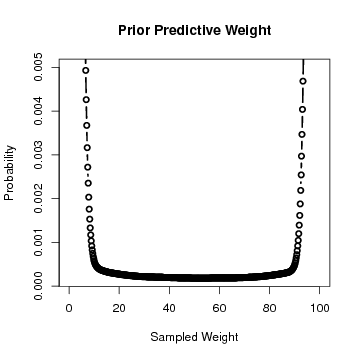
\includegraphics{./pictures/priorPredict.png}
%\caption{Prior Prediction}
%\label{priorPrediction}
%\end{figure}
%
%As seen in Figure(\ref{priorPrediction}) the prior predictive of (M4) is
%both symmetric and quite diffuse over the 100 pound domain. The U shape
%of the distribution is a side effect of the diffusion of the selected
%prior. As data are added to the model, the indecisive U shape collapses
%toward the data in the posterior.

\subsection{Appendix C: Spatial Model Averaging}\label{appBMA}

[Reiterate BMA procedure]

Figures (\ref{colorTabApp78} and \ref{colorTabApp83}) show the spatial model 
averaging results are shown for all modeled time periods (1978-1982 and 
1983-1990) in all modeled market categories. For brevity we only show the five 
most highly weighted models in each market category, although 274 candidate 
port complex partitioning schemes are computed in each market category in each 
modeled time period.  

Notice that each market category has fairly unique port complex
partitioning results. The fact that each market category behaves
uniquely indicates the complexity of this system. Furthermore the fact
that the BMA strategy picks up on these varied market category
behaviors indicates the flexibility of this approach. Although the
system is very dynamic, key breaks along California biogeographic
features, such as Cape Mendocino and/or Point Conception, seem to be
recurrent patterns.

[Elaborate here with examples from each time period]

%
\clearpage
%

\subsection{Appendix D: Nuisance Parameters}\label{appNu}

Tables (\ref{rho78} - \ref{v83}) Summarize nuisance parameter posteriors for model M4 fitted
in each market category, in each modeled period. Recall high values of
\(\rho\) indicate overdispersion relative to the binomial model, and
small values of \(v\) indicate a high degree of temporal pooling in the
\(\beta^{(y:q)}_{m\eta}\) parameters.

\subsubsection{Overdispersion Parameter(\(\rho\))}

In general \(\rho\) estimates seem to account for a fair degree of
overdispersion. Values of \(\rho\) never approach the maximal limit
(\(\rho=1\)), and thus the beta-binomial model seems to be appropriately
to modeling the observed residual variance of these data, on average,
without structurally underestimating variability.

%
\begin{table}[h!]
\begin{minipage}[c]{0.45\textwidth}
\centering
$~$\\$~$\\$~$\\
\begin{tabular}{cccc}
\hline
MCAT & Mean & Median & SD     \\ \hline
250 & 0.55 & 0.55 & 0.004       \\
253 & 0.39 & 0.39 & 0.001       \\
262 & 0.35 & 0.35 & 0.008       \\
265 & 0.64 & 0.64 & 0.002       \\
269 & 0.52 & 0.52 & 0.019       \\
270 & 0.53 & 0.54 & 0.020       \\
956 & 0.35 & 0.35 & 0.007       \\
959 & 0.47 & 0.47 & 0.070       \\
961 & 0.55 & 0.55 & 0.004       \\
\hline
\end{tabular}
$~$\\$~$\\$~$\\$~$\\
\caption{1978-1982: $\rho$ posterior mean, median, and standard deviation summaries for 
all modeled market categories.}% in the 1978-1982 time period.}
\label{rho78}
%\end{table}
\end{minipage}
\begin{minipage}[c]{0.09\textwidth}
$~$
\end{minipage}
\begin{minipage}[c]{0.45\textwidth} 
%\begin{table}[h!]
\centering
\begin{tabular}{cccc}
\hline
MCAT & Mean & Median & SD     \\ \hline
245 & 0.65 & 0.65 & 0.014       \\
250 & 0.51 & 0.51 & 0.002       \\
253 & 0.47 & 0.47 & 0.010       \\
259 & 0.75 & 0.75 & 0.009       \\
262 & 0.41 & 0.41 & 0.001       \\
269 & 0.57 & 0.57 & 0.046       \\
270 & 0.74 & 0.75 & 0.027       \\
663 & 0.51 & 0.51 & 0.001       \\
667 & 0.49 & 0.49 & 0.022       \\
956 & 0.43 & 0.43 & 0.003       \\
959 & 0.55 & 0.55 & 0.004       \\
960 & 0.45 & 0.45 & 0.004       \\
961 & 0.59 & 0.59 & 0.001       \\
\hline
\end{tabular}
\caption{1983-1990 $\rho$ posterior mean, median, and standard deviation 
summaries for all modeled market categories.}% in the 1983-1990 time period.}
\label{rho83}
\end{minipage} 
\end{table}

%
\clearpage
%

\subsubsection{Temporal Pooling(\(v\))}\label{temporal-pooling-v}

Each modeled market category and time period require a different degree
of pooling. The variance estimates span 2 orders of magnitudes with the
smallest estimate (indicating the most temporal shrinkage) occurring in
market category 250 in 1983-1990 and the largest estimate (indicating
the least temporal shrinkage) occurring in market category 269 in
1983-1990. Modeling each market category separately provides the
flexibility to separately characterize these largely distinct temporal
pooling behaviors.

%
\begin{table}[h!]
\begin{minipage}[c]{0.45\textwidth}
\centering
$~$\\$~$\\$~$\\
\begin{tabular}{cccc}
\hline
MCAT & Mean & Median & Posterior SD     \\ \hline
250 & 12915.85 & 18523.12 & 8699.87     \\
253 & 22747.87 & 23063.76 & 1535.53     \\
262 & 20254.41 & 20506.36 & 2581.87     \\
265 & 15846.22 & 16694.98 & 7601.15     \\
269 & 20135.05 & 19975.15 & 4667.11     \\
270 & 19931.96 & 19955.13 & 6033.35     \\
956 & 19659.11 & 19795.60 & 1227.99     \\
959 & 19159.69 & 13375.80 & 19256.94    \\
961 & 18631.44 & 19498.31 & 7970.44     \\
\hline
\end{tabular}
$~$\\$~$\\$~$\\
\caption{1978-1982 $v$ posterior mean, median, and standard deviation 
summaries for all modeled market categories.}
\label{v78}
%\end{table}
\end{minipage}
\begin{minipage}[c]{0.09\textwidth}
$~$
\end{minipage}
\begin{minipage}[c]{0.45\textwidth}
%\begin{table}[h!]
\centering
\begin{tabular}{cccc}
\hline
MCAT & Mean & Median & Posterior SD     \\ \hline
245 & 20211.82 & 20204.95 & 1276.83     \\
250 & 236.03   & 192.53   & 134.67      \\
253 & 20455.18 & 20140.50 & 1521.72     \\
259 & 20246.14 & 20186.61 & 898.99      \\
262 & 20445.49 & 20348.56 & 343.70      \\
269 & 34386.49 & 25951.03 & 24030.32    \\
270 & 20253.34 & 19908.07 & 9269.02     \\
663 & 19563.87 & 19624.09 & 331.04      \\
667 & 20089.55 & 20078.27 & 2723.34     \\
956 & 20581.67 & 20664.71 & 913.92      \\
959 & 19242.41 & 18707.09 & 5076.03     \\
960 & 20059.66 & 20012.80 & 1703.89     \\
961 & 20127.69 & 20141.04 & 580.80      \\
\hline
\end{tabular}
\caption{1983-1990 $v$ posterior mean, median, and standard deviation  
summaries for all modeled market categories.}
\label{v83}
\end{minipage}
\end{table}

\clearpage

%
%
\section{Figures}
%
%

\begin{figure}[h!]
\centering
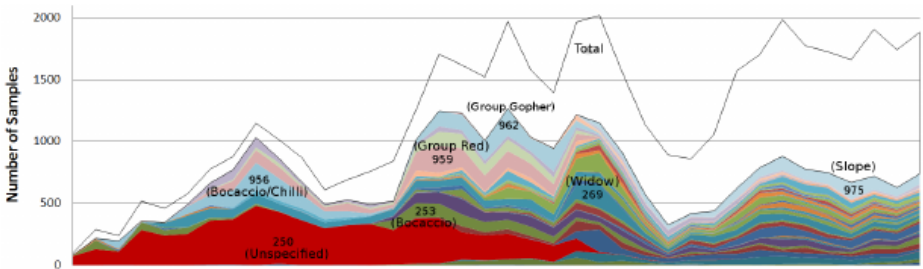
\includegraphics[width=\textwidth]{./pictures/mcatColors.png}
$~$\\
\vspace*{-2cm}
\hspace*{-0.3cm}
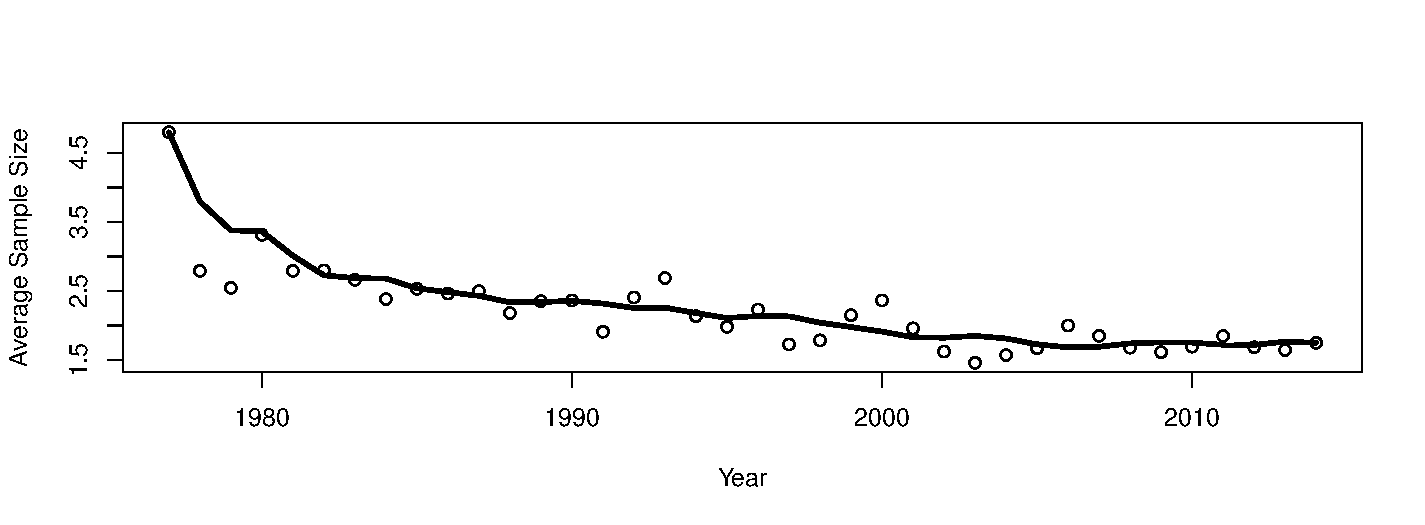
\includegraphics[width=1.055\textwidth]{./pictures/stratAvgSamp.pdf}
$~$\\
\vspace*{-3.8cm}
\hspace*{-0.3cm}
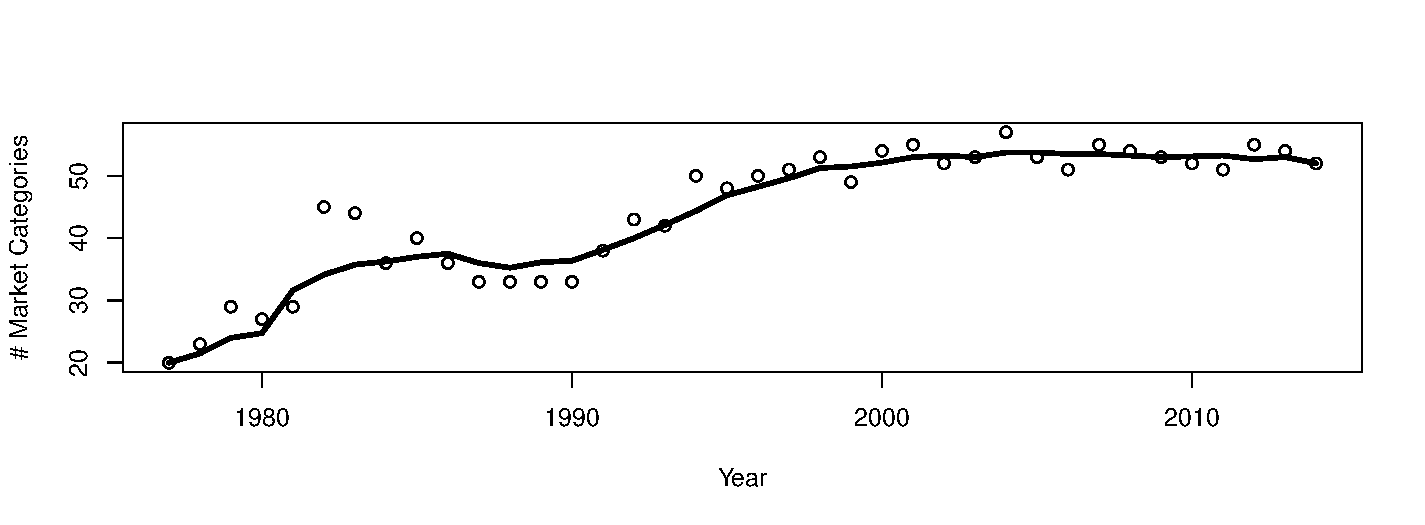
\includegraphics[width=1.055\textwidth]{./pictures/nMcatsEMA.pdf}
\caption{Number of commercial port samples per market
category in California, 1978-2014 (upper panel), average sample size per
stratum (middle panel), and number of market categories recorded on
landing receipts (lower panel). On the lower panels, points indicate
observed values, while the black lines represent 9 year moving averages}
\label{sparceData}
%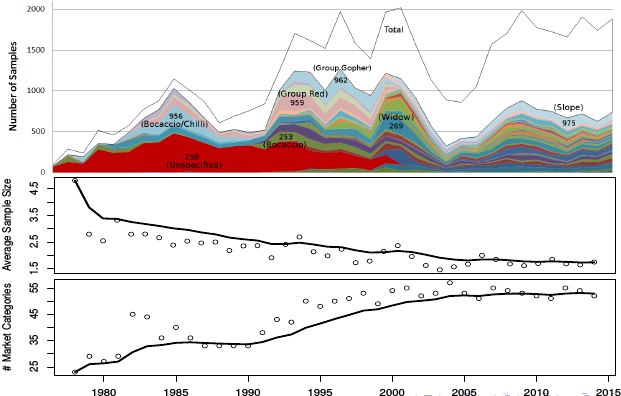
\includegraphics[width=\textwidth]{./pictures/sampleComplex.png}
\end{figure}

\begin{landscape}
\begin{figure}
\centering
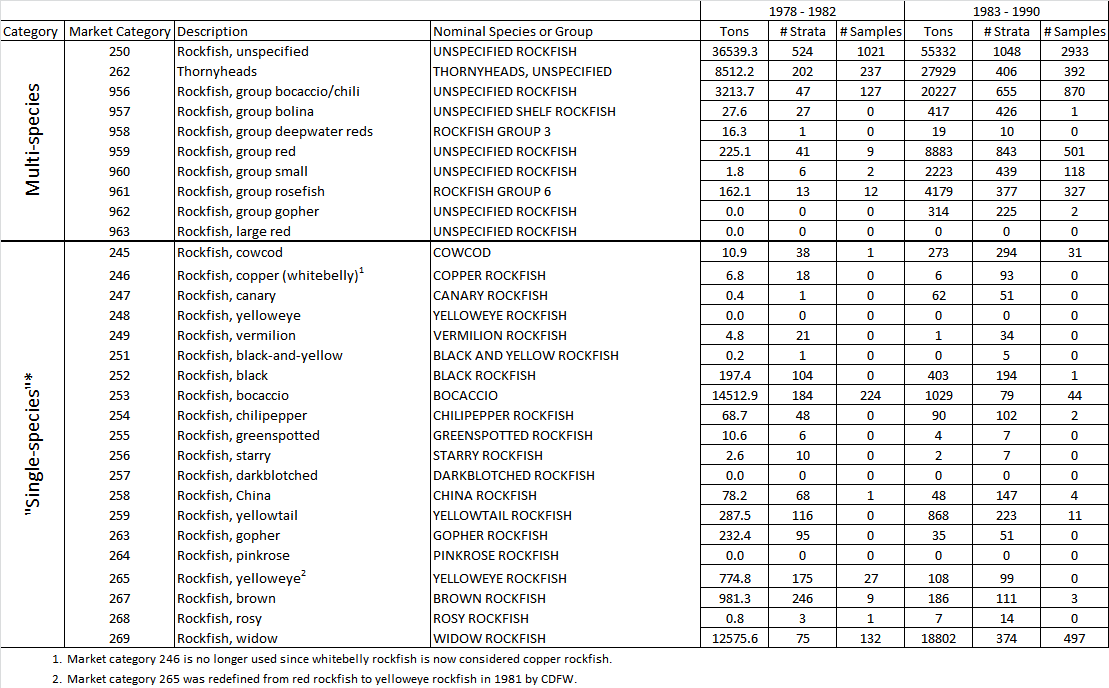
\includegraphics[width=1.3\textwidth]{./pictures/MC_summary_table_part_1.png}
%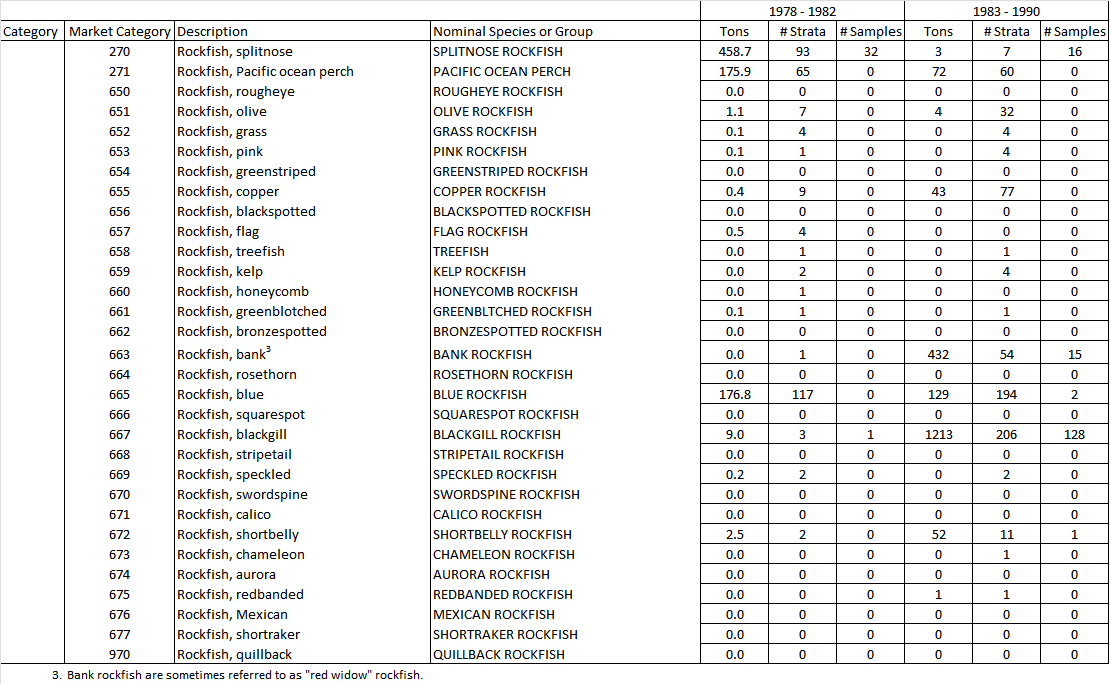
\includegraphics[width=\textwidth]{./pictures/MC_summary_table_part_2.png}
\caption{Landed weight (metric tons), number of landed strata (year, quarter, 
port complex, and gear group), and number of species composition samples by 
market category and time period. Market categories created after 1990 are not 
listed (e.g. 678, 679, 964, and 971-976). *"Single-species" market categories 
are nominal (in name only); landings in these categories often include a 
mixture of species.}
\label{ej1}
\end{figure}
\end{landscape}

\begin{landscape}
\begin{figure}
\centering
%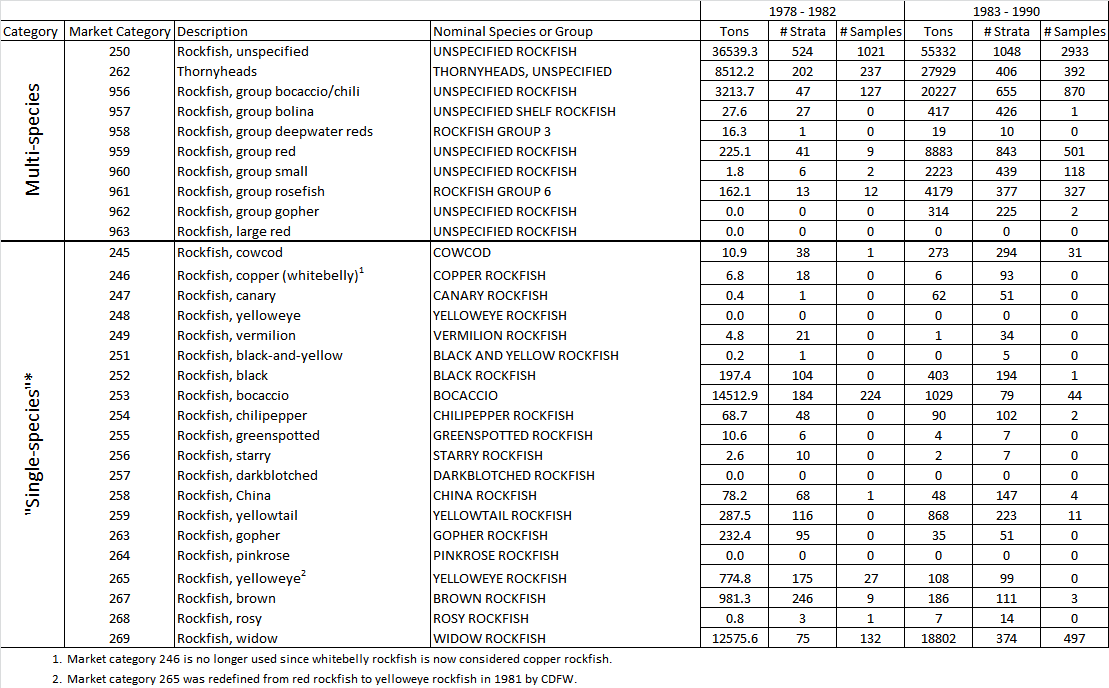
\includegraphics[width=\textwidth]{./pictures/MC_summary_table_part_1.png}
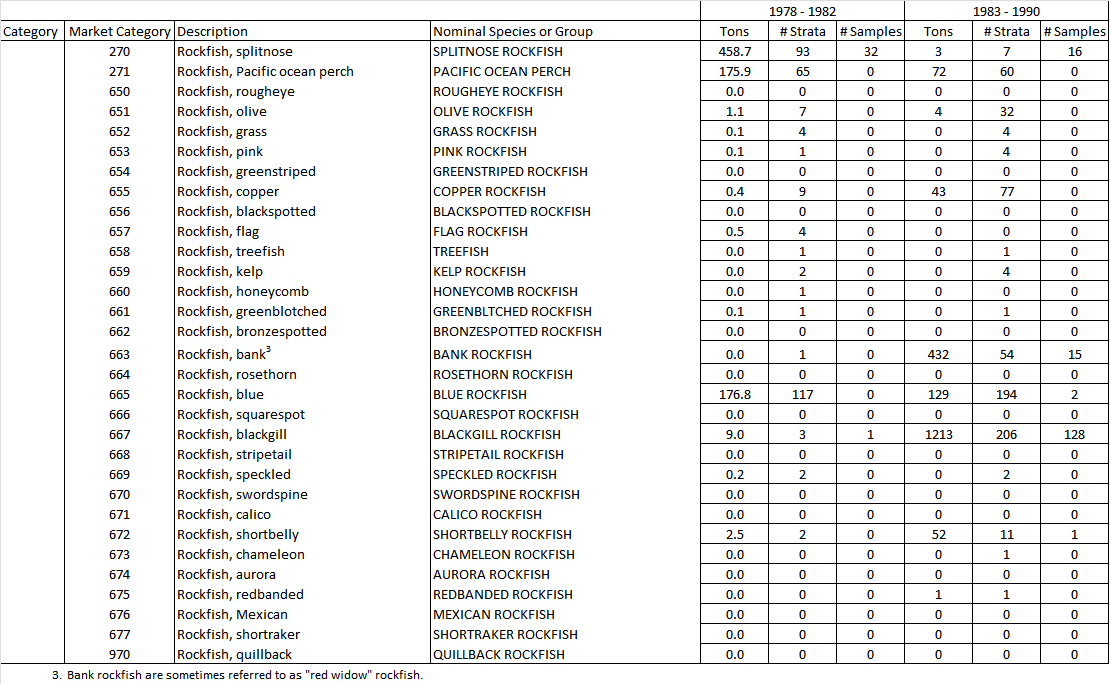
\includegraphics[width=1.3\textwidth]{./pictures/MC_summary_table_part_2.png}
\caption{Landed weight (metric tons), number of landed strata (year, quarter, 
port complex, and gear group), and number of species composition samples by 
market category and time period. Market categories created after 1990 are not 
listed (e.g. 678, 679, 964, and 971-976). *"Single-species" market categories 
are nominal (in name only); landings in these categories often include a 
mixture of species.}
\label{ej2}
\end{figure}
\end{landscape}

%
\begin{figure}[h!]
\centering
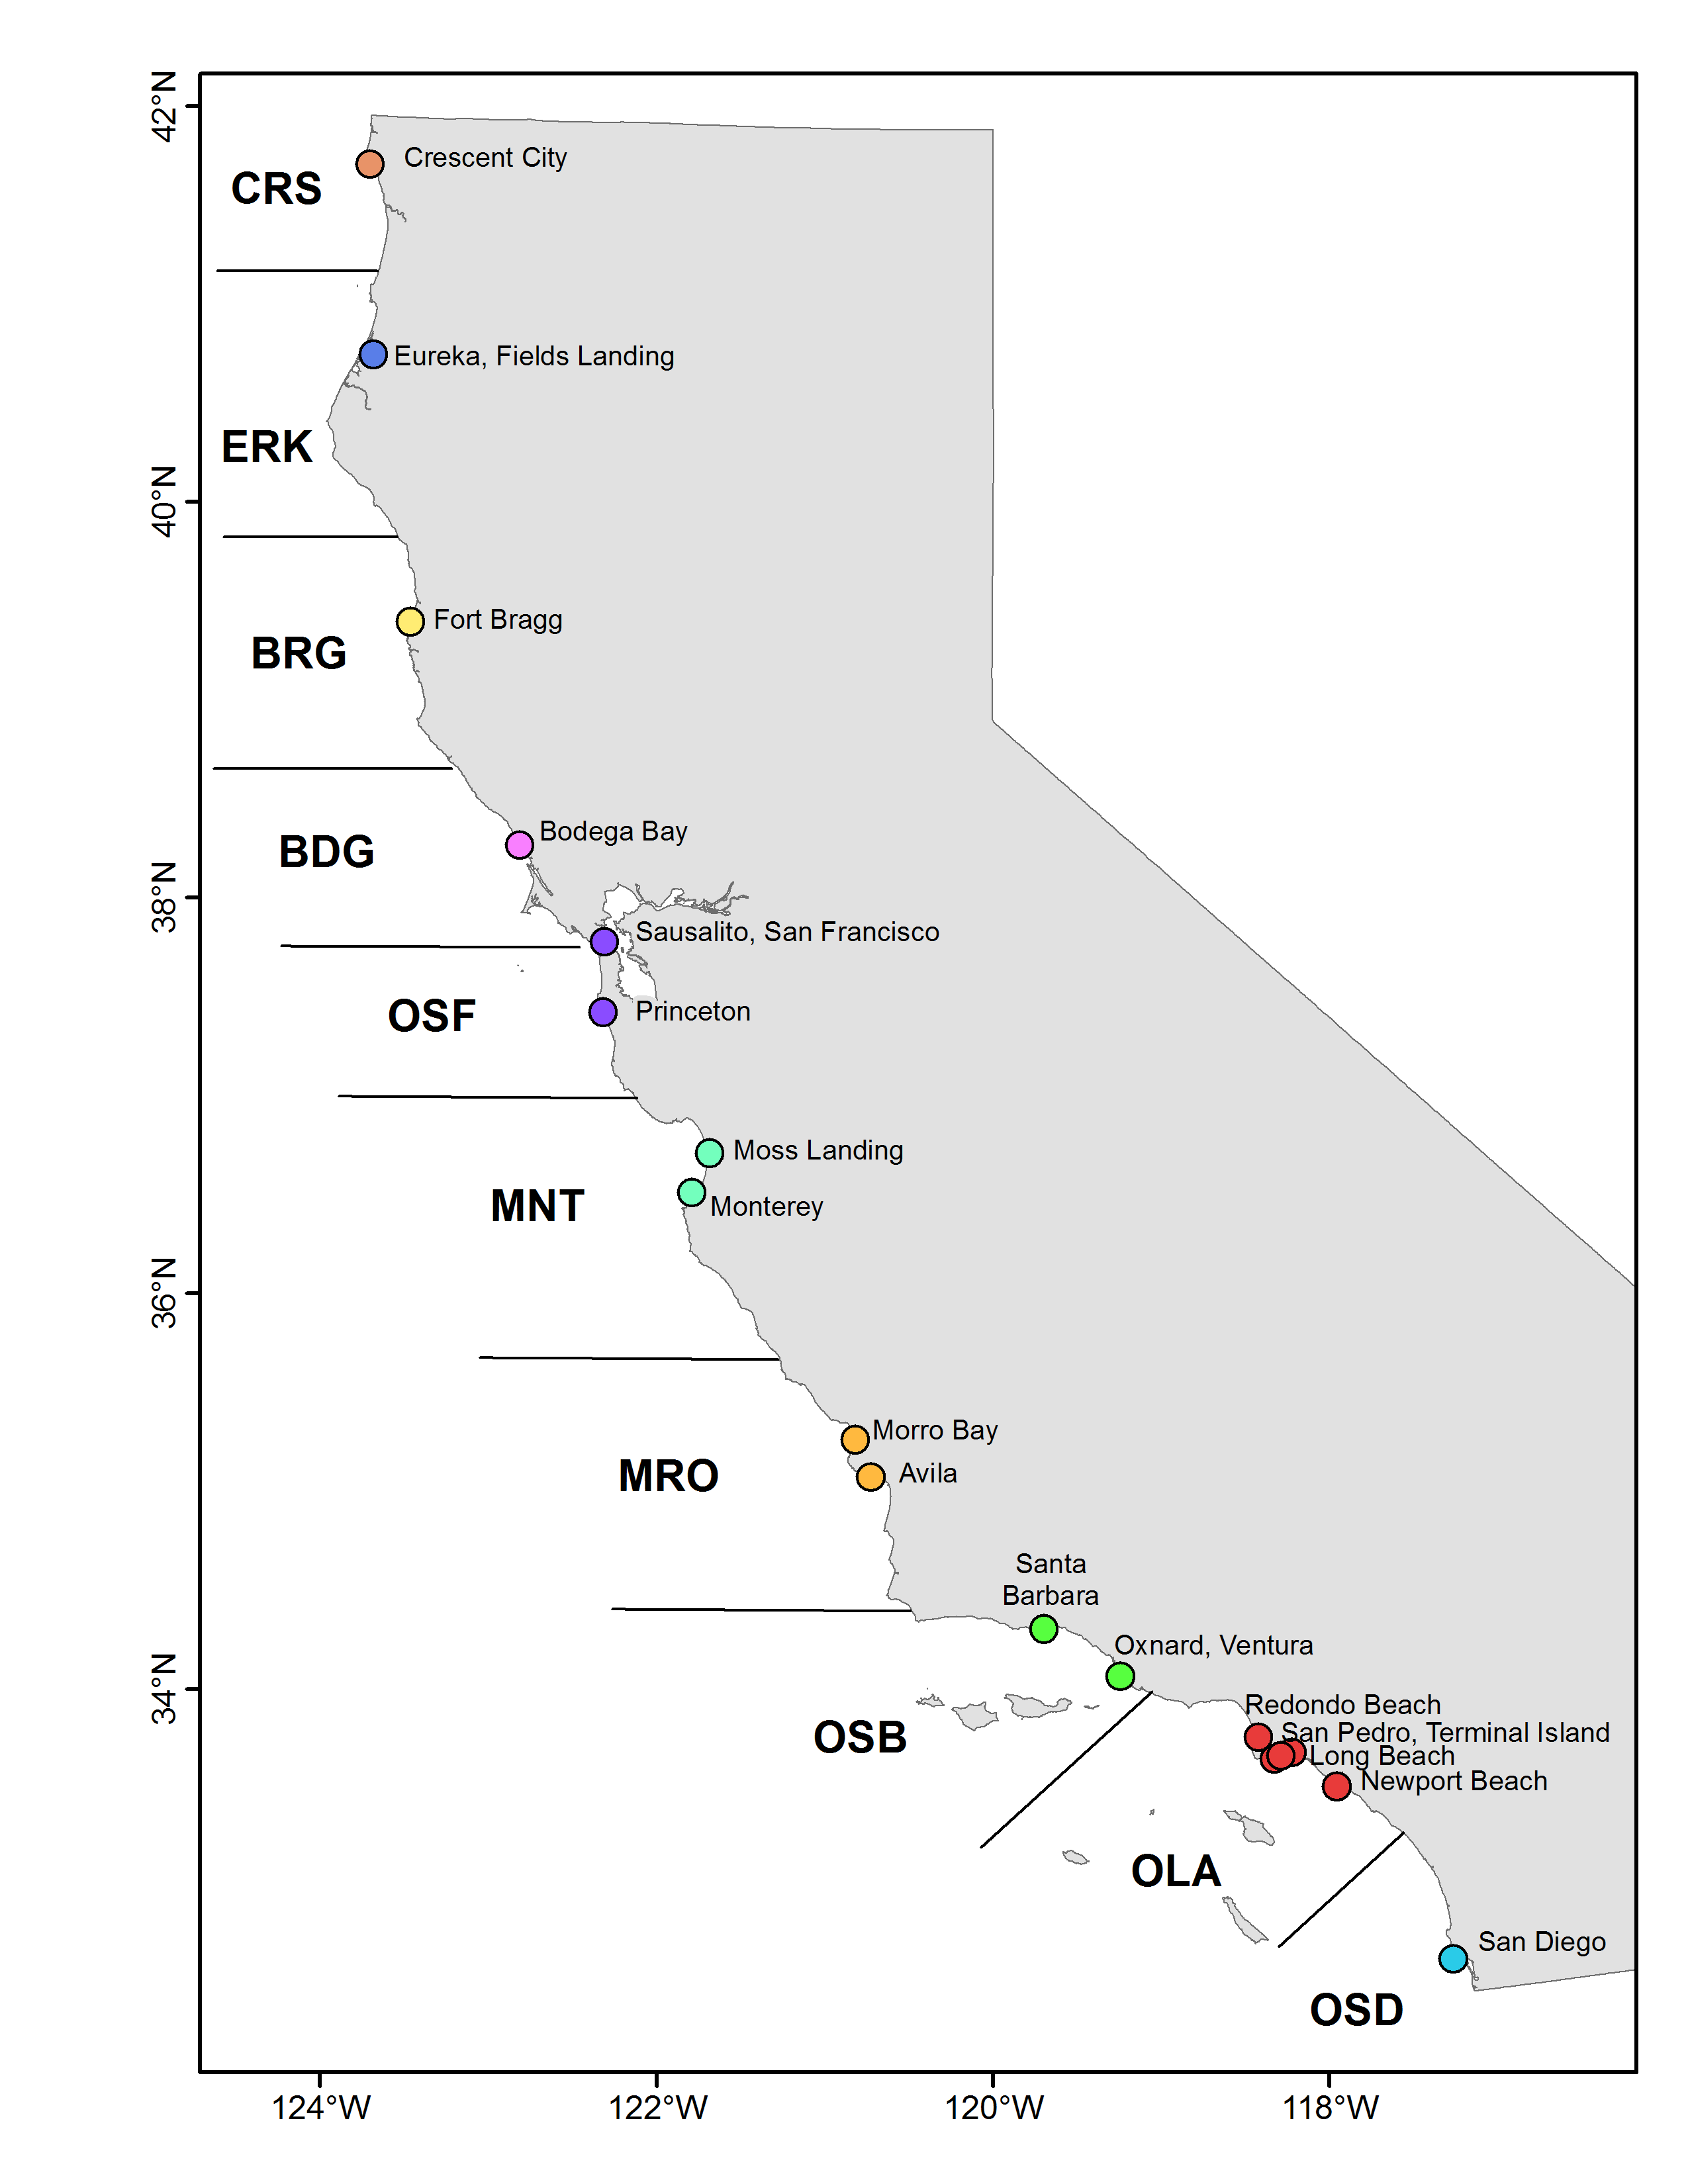
\includegraphics[width=\textwidth]{./pictures/COMX_Ports_Final.png}
\caption{Map showing the ports in California that account for at least 95\% of 
landings. Separating lines show how ports have been aggregated into port 
complexes.}
\label{portMap}
\end{figure}

%
%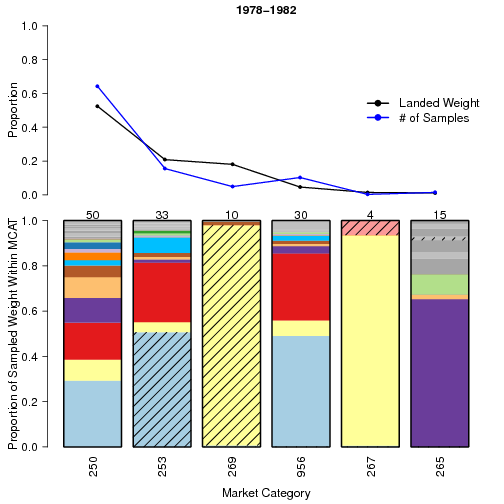
\includegraphics{./pictures/1978to1982Bar3.png}
%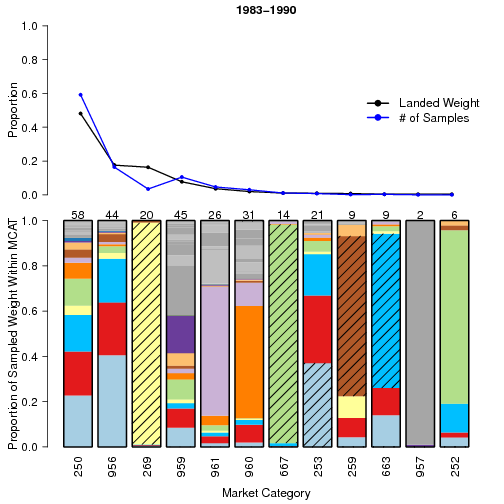
\includegraphics{./pictures/1983to1990Bar3.png}
%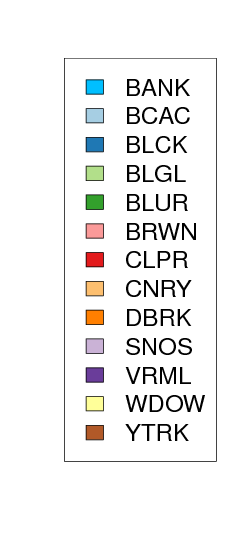
\includegraphics{./pictures/barplotLegend.png}
\begin{landscape}
\begin{figure}[h!]
\centering
\vspace{-1.2cm}
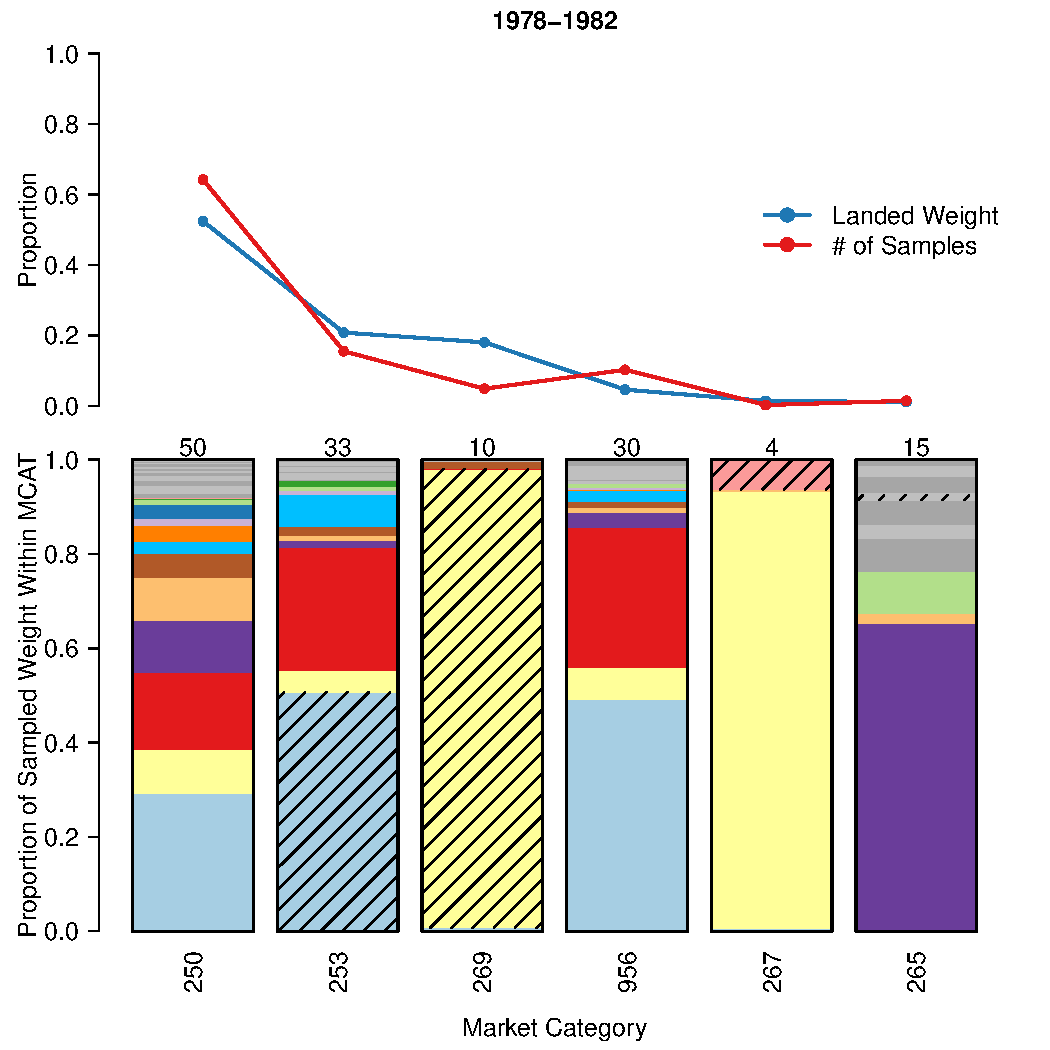
\includegraphics[height=\textheight]{./pictures/1978to1982Bar3.pdf}
%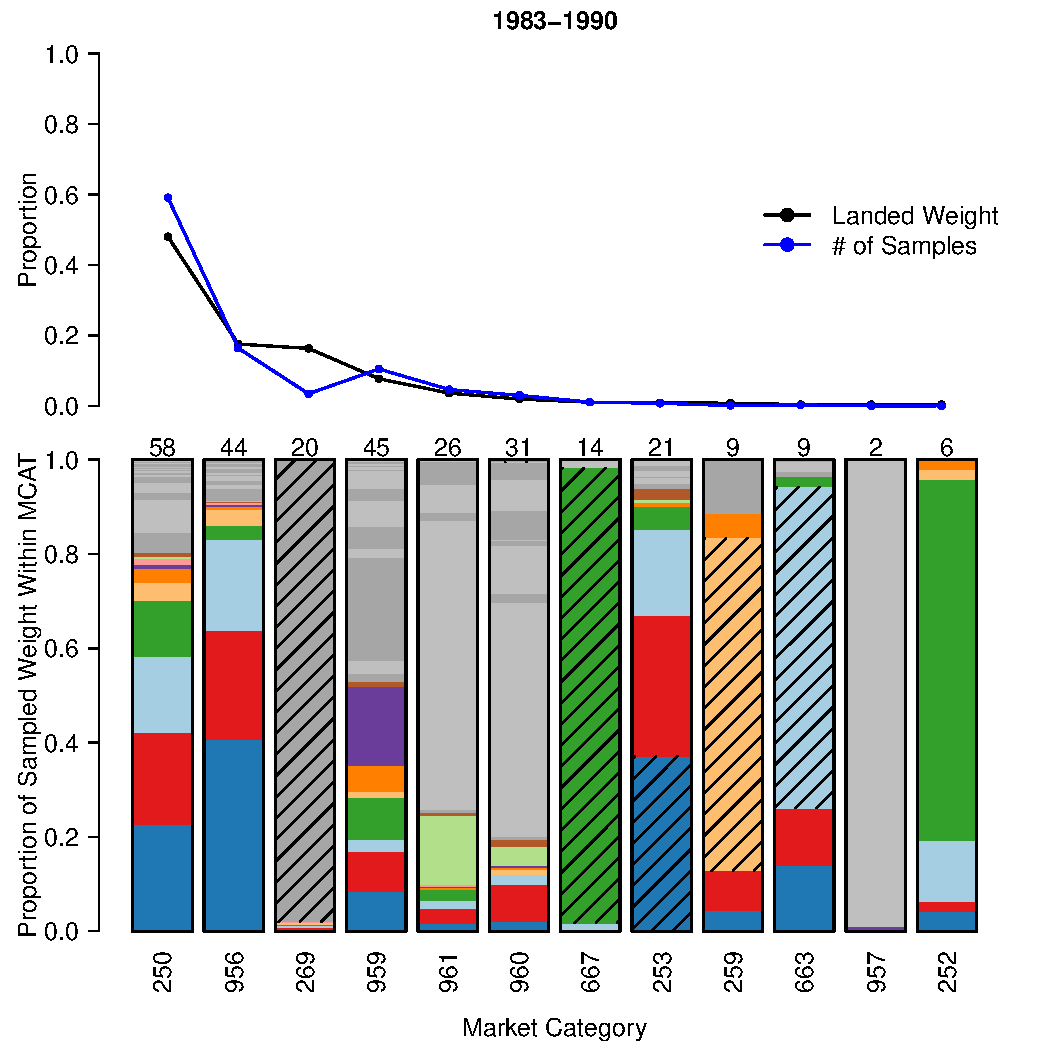
\includegraphics[width=0.43\textwidth]{./pictures/1983to1990Bar3.pdf}
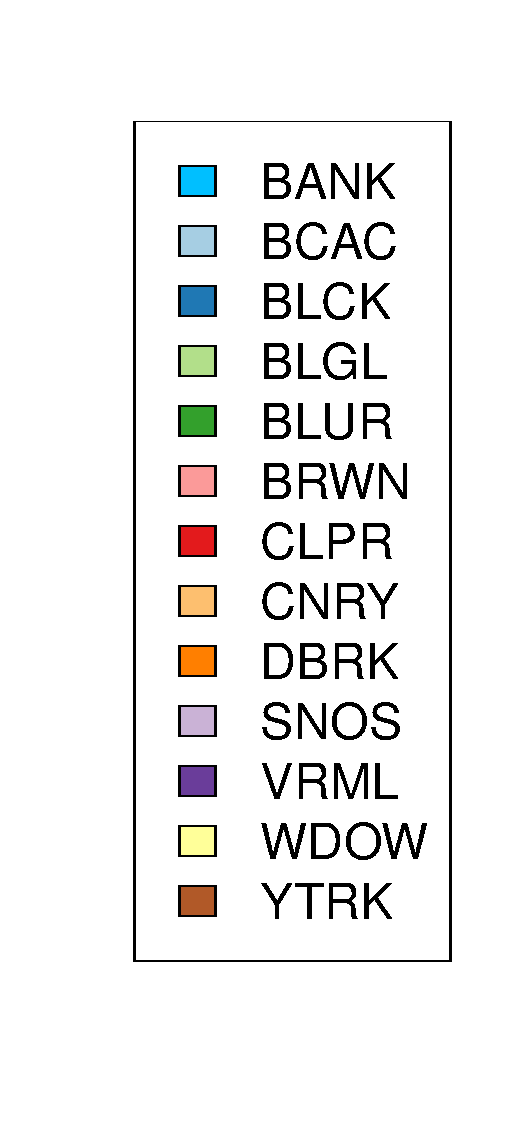
\includegraphics[height=0.8\textheight]{./pictures/barplotLegend.pdf}
\caption{Upper panel shows the proportion of landed weight (black) and number of 
samples (blue) in each market category for the 1978-1982 time period. Bottom panel 
shows the proportion of sampled weight for each species in each market category 
shown. The number above each colored bar indicated the number of species in 
the market category. Hashing indicates the species that is nominal in relevant 
the market category.}
\label{bar78}
\end{figure}
\end{landscape}

%
\clearpage
%

\begin{landscape}
\begin{figure}[h!]
\centering
\vspace{-1.2cm}
%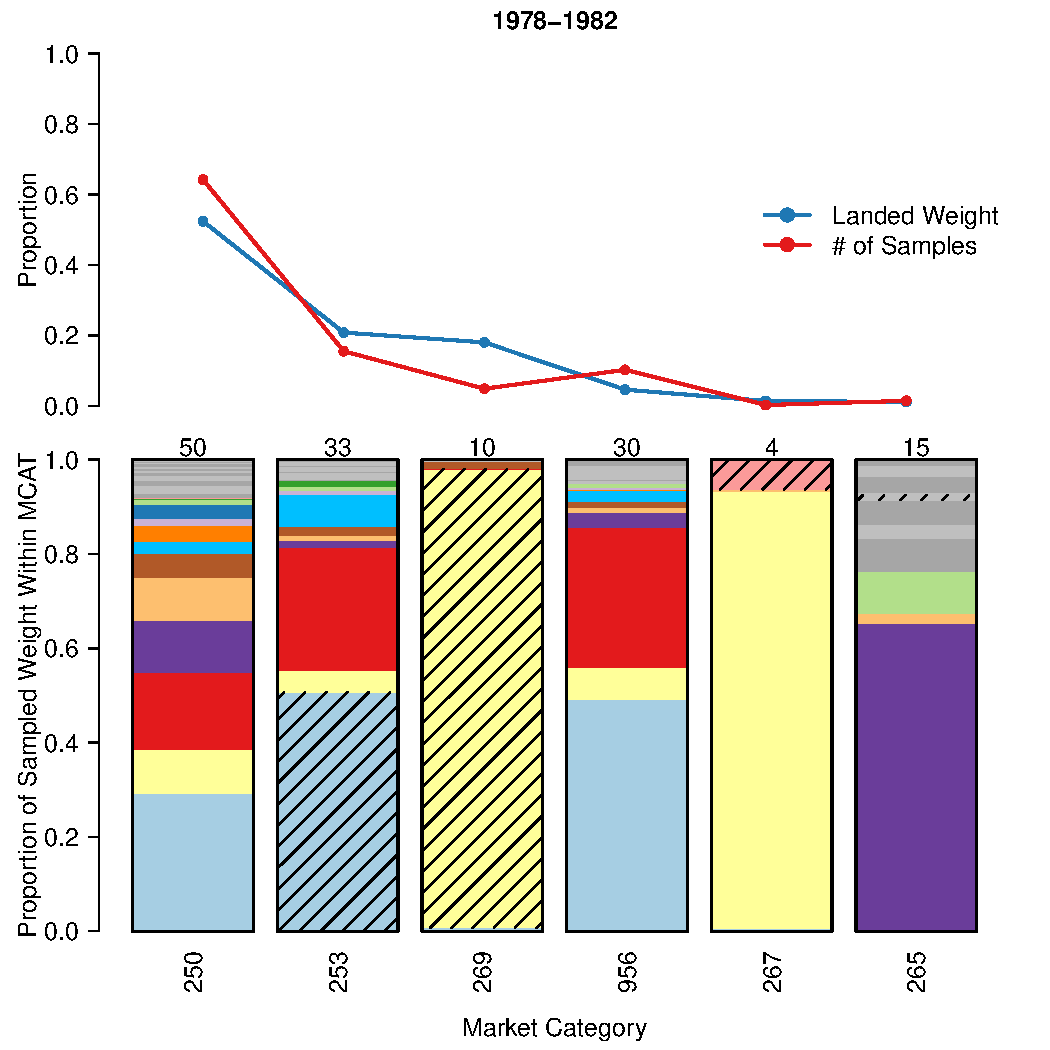
\includegraphics[height=\textheight]{./pictures/1978to1982Bar3.pdf}
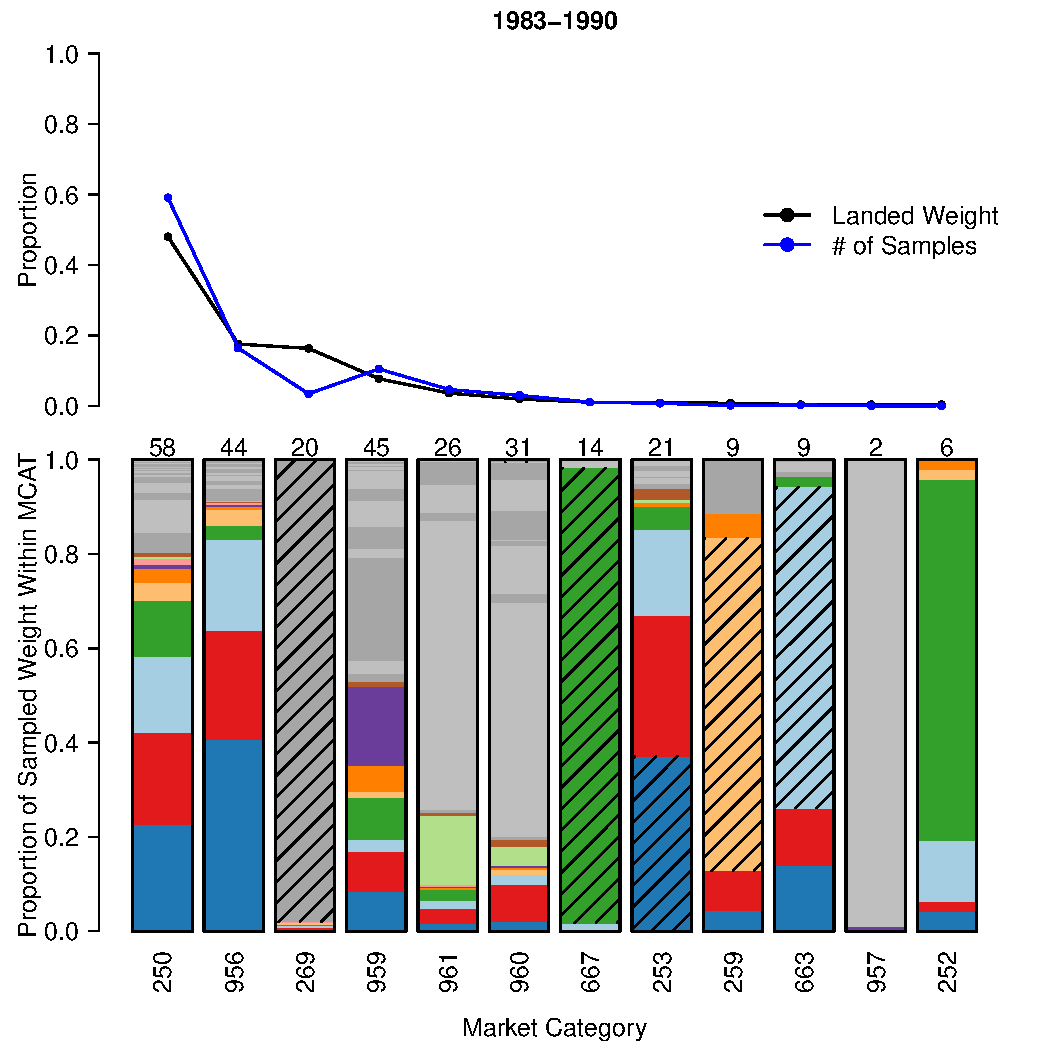
\includegraphics[height=\textheight]{./pictures/1983to1990Bar3.pdf}
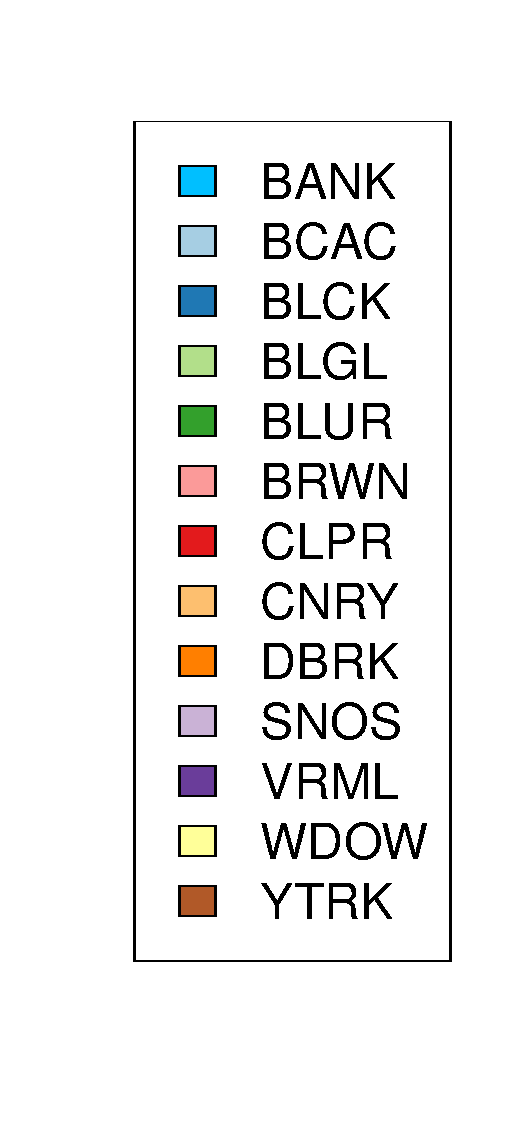
\includegraphics[height=0.8\textheight]{./pictures/barplotLegend.pdf}
\caption{Upper panel shows the proportion of landed weight (black) and number of                 
samples (blue) in each market category for the 1983-1990 time period. Bottom panel 
shows the proportion of sampled weight for each species in each market category 
shown. The number above each colored bar indicated the number of species in 
the market category. Hashing indicates the species that is nominal in relevant 
the market category.}
\label{bar83}
\end{figure}
\end{landscape}

%
\clearpage
%

\begin{landscape}
\begin{figure}[h!]
\centering
\vspace{-1.2cm}
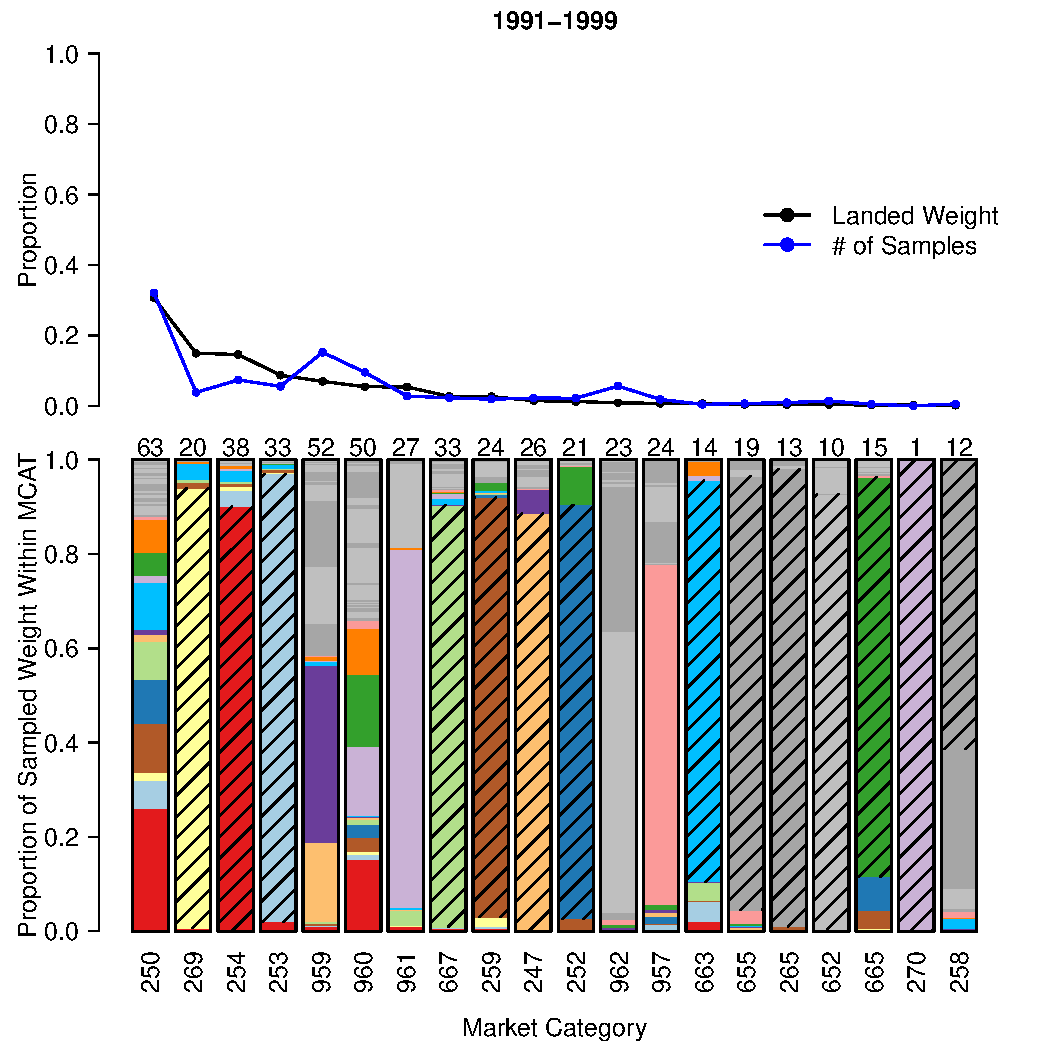
\includegraphics[height=\textheight]{./pictures/1991to1999Bar3.pdf}
%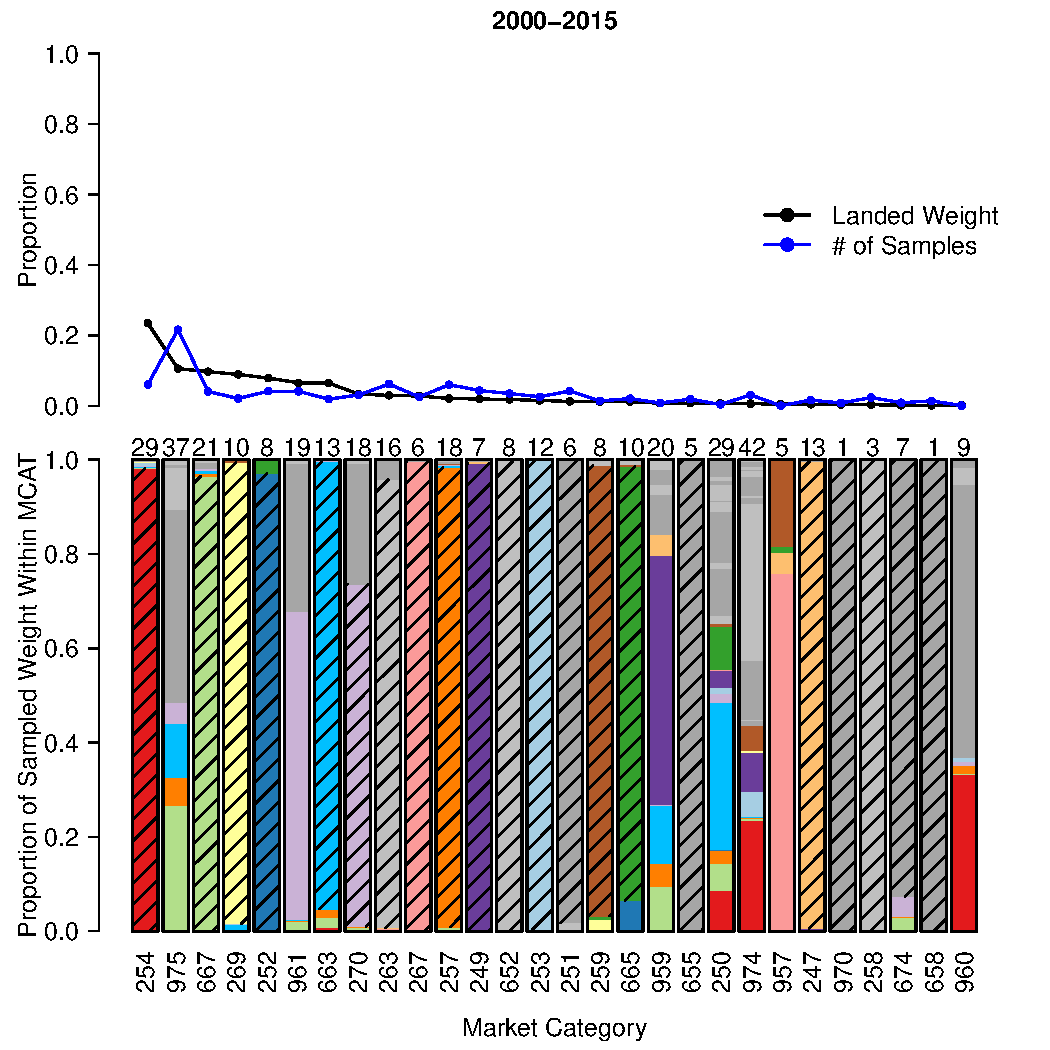
\includegraphics[width=0.43\textwidth]{./pictures/2000to2015Bar3.pdf}
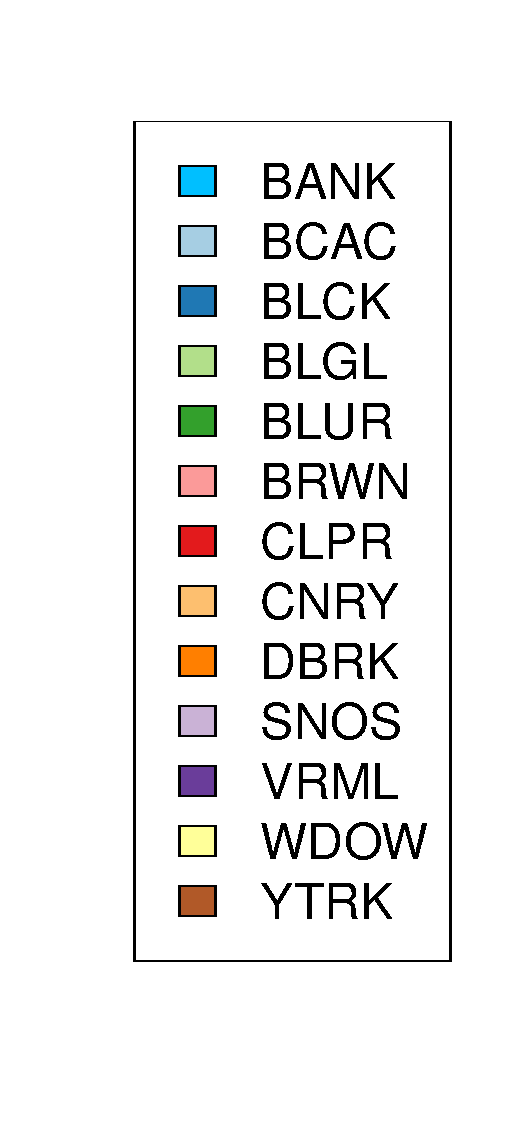
\includegraphics[height=0.8\textheight]{./pictures/barplotLegend.pdf}
\caption{Upper panel shows the proportion of landed weight (black) and number of                 
samples (blue) in each market category for the 1991-1999 time period. Bottom panel 
shows the proportion of sampled weight for each species in each market category 
shown. The number above each colored bar indicated the number of species in 
the market category. Hashing indicates the species that is nominal in relevant 
the market category.}
\label{bar91}
\end{figure}
\end{landscape}

%
\clearpage
%

\begin{landscape}
\begin{figure}[h!]
\centering
\vspace{-1.2cm}
%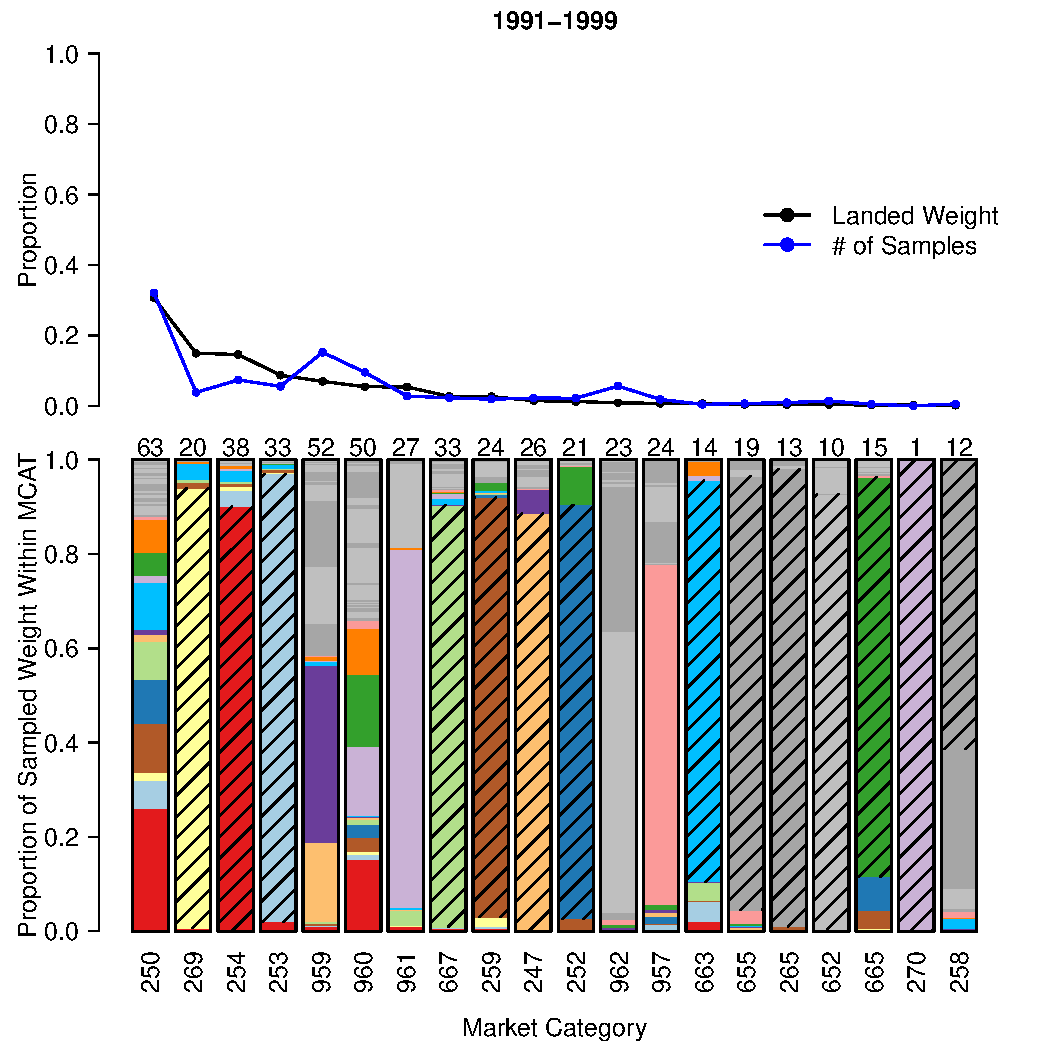
\includegraphics[width=0.43\textwidth]{./pictures/1991to1999Bar3.pdf}
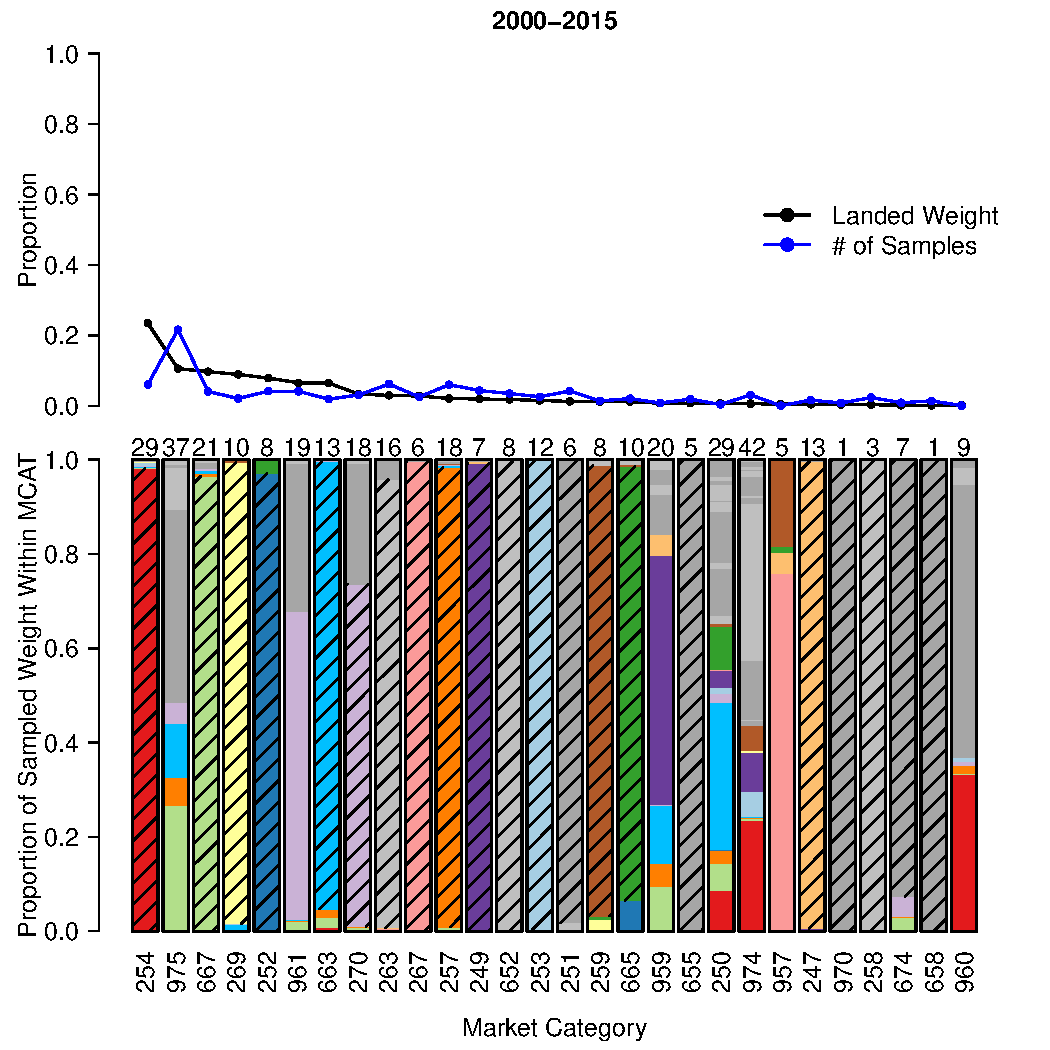
\includegraphics[height=\textheight]{./pictures/2000to2015Bar3.pdf}
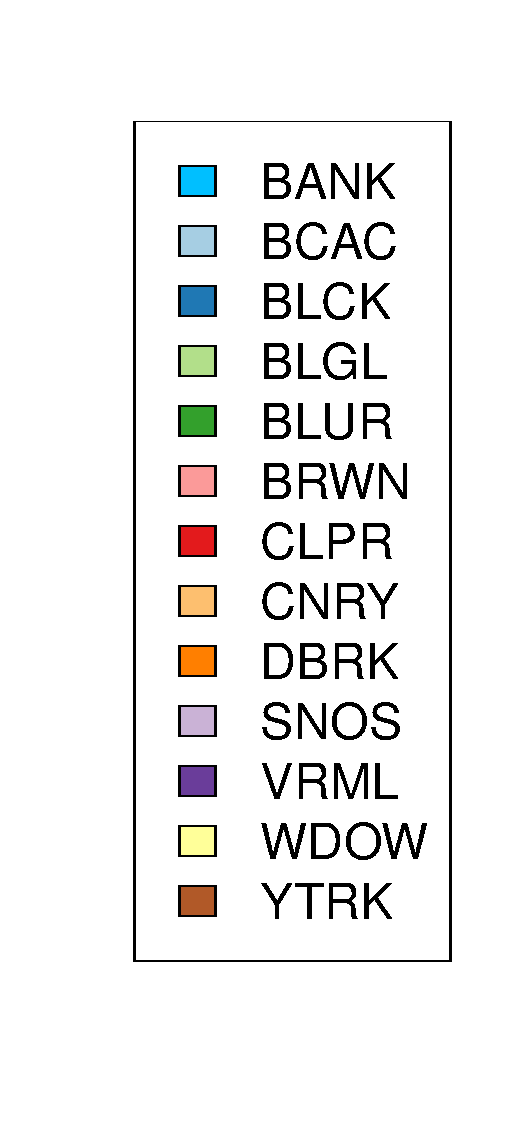
\includegraphics[height=0.8\textheight]{./pictures/barplotLegend.pdf}
\caption{Upper panel shows the proportion of landed weight (black) and number of                 
samples (blue) in each market category for the 2000-2015 time period. Bottom panel 
shows the proportion of sampled weight for each species in each market category 
shown. The number above each colored bar indicated the number of species in 
the market category. Hashing indicates the species that is nominal in relevant 
the market category.}
\label{bar00}
\end{figure}
\end{landscape}

%
\clearpage
%

%
\begin{landscape}
\begin{figure}[!h]
\centering
\resizebox{1.3\textwidth}{!}{\begin{tabular}{|c|c|c|c|c|c|c|c|c|c|c|}
        %\hline \multicolumn{6}{|c|}{MCAT 250} \\ \hline
        \hline \multicolumn{11}{|c|}{MCAT 250} \\ \hline 
        %$\omega$&0.32&0.14&0.13&0.12&0.02 \\ \hline %&0.02&0.02&0.02&0.02&0.02 \\ \hline
        $\omega$&0.32&0.14&0.13&0.12&0.02&0.02&0.02&0.02&0.02&0.02 \\ \hline
        CRS&\cellcolor[HTML]{E41A1C}&\cellcolor[HTML]{E41A1C}&\cellcolor[HTML]{E41A1C}&\cellcolor[HTML]{E41A1C}&\cellcolor[HTML]{E41A1C}&\cellcolor[HTML]{E41A1C}&\cellcolor[HTML]{E41A1C}&\cellcolor[HTML]{E41A1C}&\cellcolor[HTML]{E41A1C}&\cellcolor[HTML]{E41A1C} \\ \hline%
        ERK&\cellcolor[HTML]{377EB8}&\cellcolor[HTML]{377EB8}&\cellcolor[HTML]{377EB8}&\cellcolor[HTML]{377EB8}&\cellcolor[HTML]{377EB8}&\cellcolor[HTML]{377EB8}&\cellcolor[HTML]{377EB8}&\cellcolor[HTML]{377EB8}&\cellcolor[HTML]{377EB8}&\cellcolor[HTML]{377EB8} \\ \hline%
        BRG&\cellcolor[HTML]{4DAF4A}&\cellcolor[HTML]{4DAF4A}&\cellcolor[HTML]{4DAF4A}&\cellcolor[HTML]{4DAF4A}&\cellcolor[HTML]{4DAF4A}&\cellcolor[HTML]{4DAF4A}&\cellcolor[HTML]{4DAF4A}&\cellcolor[HTML]{4DAF4A}&\cellcolor[HTML]{4DAF4A}&\cellcolor[HTML]{4DAF4A} \\ \hline%
        BDG&\cellcolor[HTML]{4DAF4A}&\cellcolor[HTML]{4DAF4A}&\cellcolor[HTML]{4DAF4A}&\cellcolor[HTML]{4DAF4A}&\cellcolor[HTML]{4DAF4A}&\cellcolor[HTML]{4DAF4A}&\cellcolor[HTML]{4DAF4A}&\cellcolor[HTML]{984EA3}&\cellcolor[HTML]{4DAF4A}&\cellcolor[HTML]{4DAF4A} \\ \hline%
        OSF&\cellcolor[HTML]{984EA3}&\cellcolor[HTML]{984EA3}&\cellcolor[HTML]{984EA3}&\cellcolor[HTML]{984EA3}&\cellcolor[HTML]{4DAF4A}&\cellcolor[HTML]{4DAF4A}&\cellcolor[HTML]{4DAF4A}&\cellcolor[HTML]{984EA3}&\cellcolor[HTML]{4DAF4A}&\cellcolor[HTML]{4DAF4A} \\ \hline%
        MNT&\cellcolor[HTML]{984EA3}&\cellcolor[HTML]{984EA3}&\cellcolor[HTML]{984EA3}&\cellcolor[HTML]{984EA3}&\cellcolor[HTML]{984EA3}&\cellcolor[HTML]{984EA3}&\cellcolor[HTML]{984EA3}&\cellcolor[HTML]{FF7F00}&\cellcolor[HTML]{984EA3}&\cellcolor[HTML]{984EA3} \\ \hline%
        MRO&\cellcolor[HTML]{984EA3}&\cellcolor[HTML]{984EA3}&\cellcolor[HTML]{984EA3}&\cellcolor[HTML]{984EA3}&\cellcolor[HTML]{984EA3}&\cellcolor[HTML]{984EA3}&\cellcolor[HTML]{984EA3}&\cellcolor[HTML]{FF7F00}&\cellcolor[HTML]{984EA3}&\cellcolor[HTML]{984EA3} \\ \hline%
        OSB&\cellcolor[HTML]{FF7F00}&\cellcolor[HTML]{FF7F00}&\cellcolor[HTML]{FF7F00}&\cellcolor[HTML]{FF7F00}&\cellcolor[HTML]{FF7F00}&\cellcolor[HTML]{FF7F00}&\cellcolor[HTML]{FF7F00}&\cellcolor[HTML]{FF7F00}&\cellcolor[HTML]{984EA3}&\cellcolor[HTML]{FF7F00} \\ \hline%
        OLA&\cellcolor[HTML]{FF7F00}&\cellcolor[HTML]{FFFF33}&\cellcolor[HTML]{FF7F00}&\cellcolor[HTML]{FFFF33}&\cellcolor[HTML]{FF7F00}&\cellcolor[HTML]{FFFF33}&\cellcolor[HTML]{FFFF33}&\cellcolor[HTML]{FFFF33}&\cellcolor[HTML]{FF7F00}&\cellcolor[HTML]{FF7F00} \\ \hline%
        OSD&\cellcolor[HTML]{FF7F00}&\cellcolor[HTML]{FFFF33}&\cellcolor[HTML]{FFFF33}&\cellcolor[HTML]{A65628}&\cellcolor[HTML]{FFFF33}&\cellcolor[HTML]{FFFF33}&\cellcolor[HTML]{A65628}&\cellcolor[HTML]{FFFF33}&\cellcolor[HTML]{FFFF33}&\cellcolor[HTML]{FF7F00} \\ \hline%
\end{tabular}}
$~$\\$~$\\$~$\\
\caption{The model averaging results of port complex model selection for 
market category 250 in 1978 to 1982. BMA weights (\(\omega\)) for the top 10 
models are displayed in the top row (each column is a distinct model). The 
following ten rows indicate the ten port complexes in California, and the 
colored cells indicate how port complexes are partitioned in each model.}
\label{colorTab78}
\end{figure}
\end{landscape}

%
\clearpage
%

\begin{figure}[h!]
\centering
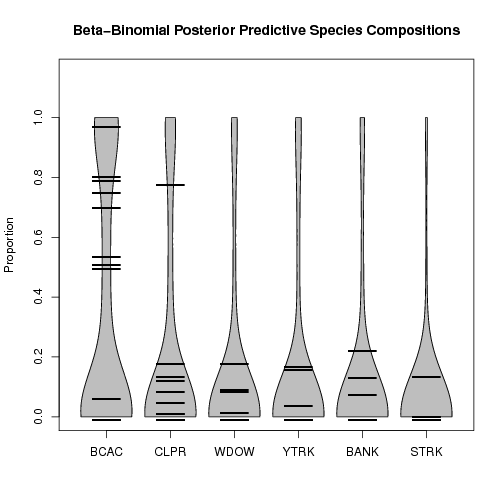
\includegraphics{./pictures/compVioplotQtr2.png}
\caption{ A violin plot of the beta-binomial predictive distributions 
for the six most prevalent species in the market category 250, Monterey trawl 
fishery for the second quarter of 1982. Observed species compositions, from 
port sampling, are plotted atop each density.
}
\label{violin}
\end{figure}

%
\clearpage
%

\begin{figure}[h!]
\centering
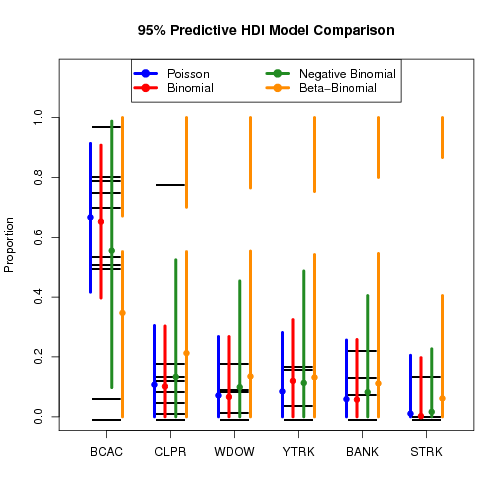
\includegraphics{./pictures/compPlot1982Qtr2.png}
\caption{Interval Plot: The predictive species composition distributions
as 95\% Highest Density Intervals (HDI) (colored vertical lines),
plotted on top of the predictive means for each model and the observed
species compositions (black horizontal lines) from the data}
\label{interval}
\end{figure}

%
\clearpage
%

%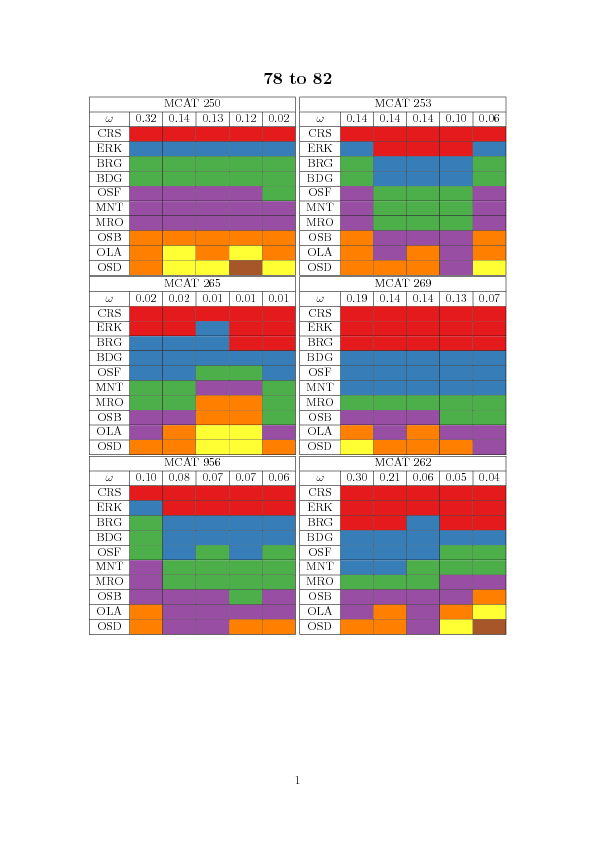
\includegraphics{./pictures/latexTableCompress1.png}
%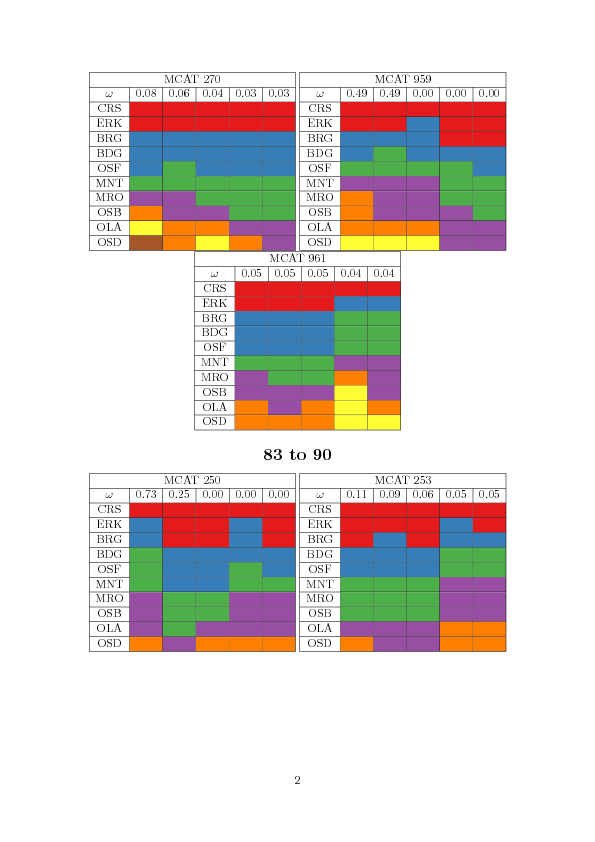
\includegraphics{./pictures/latexTableCompress2.png}
%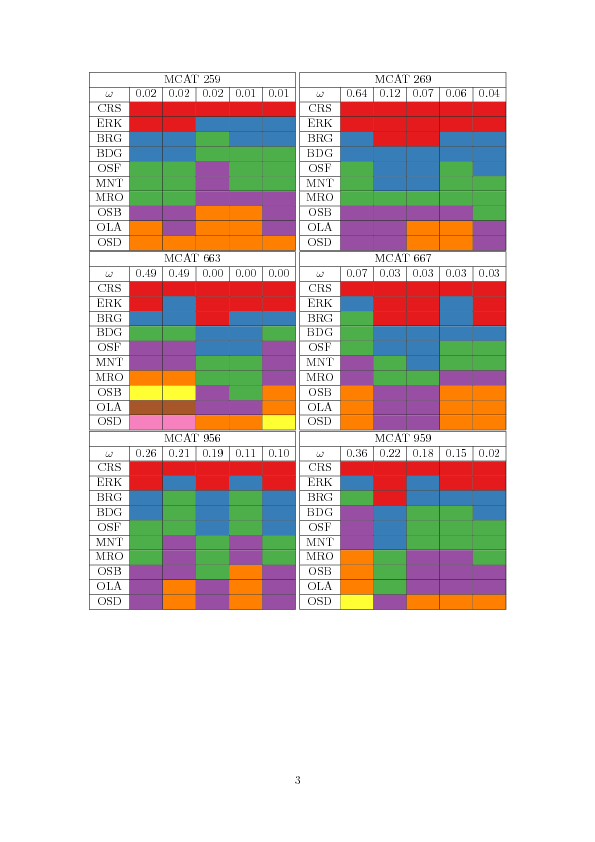
\includegraphics{./pictures/latexTableCompress3.png}
%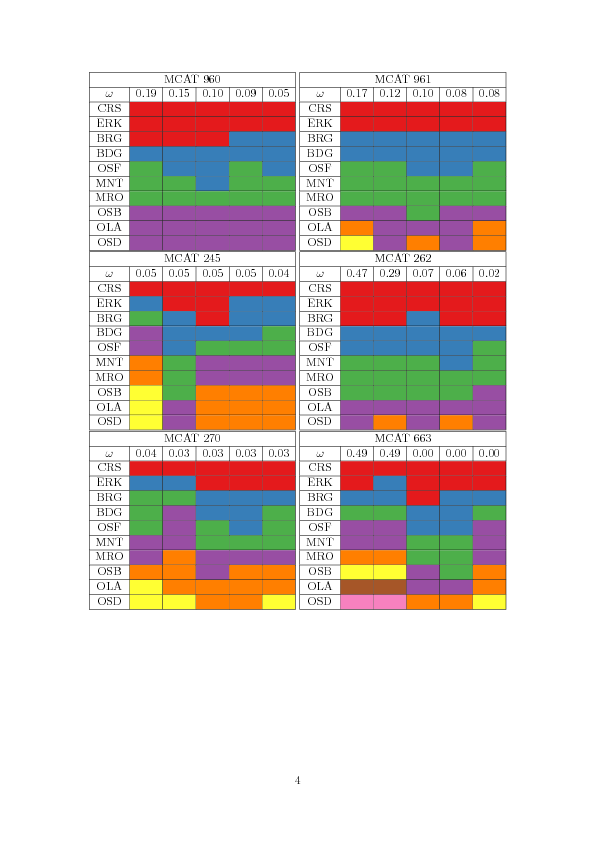
\includegraphics{./pictures/latexTableCompress4.png}
\begin{landscape}
\begin{figure}
\vspace*{-2.1cm}
\hspace*{5cm}
\begin{minipage}[c]{0.3\textwidth}
\hspace*{-5cm}
\begin{tabular}{|c|c|c|c|c|c|c|c|c|c|c|}
        \hline \multicolumn{6}{|c|}{MCAT 250} \\ \hline
        %\hline \multicolumn{11}{|c|}{MCAT 250} \\ \hline 
        $\omega$&0.32&0.14&0.13&0.12&0.02 \\ \hline %&0.02&0.02&0.02&0.02&0.02 \\ \hline
        %$\omega$&0.32&0.14&0.13&0.12&0.02&0.02&0.02&0.02&0.02&0.02 \\ \hline
        CRS&\cellcolor[HTML]{E41A1C}&\cellcolor[HTML]{E41A1C}&\cellcolor[HTML]{E41A1C}&\cellcolor[HTML]{E41A1C}&\cellcolor[HTML]{E41A1C}\\ \hline %&\cell
        ERK&\cellcolor[HTML]{377EB8}&\cellcolor[HTML]{377EB8}&\cellcolor[HTML]{377EB8}&\cellcolor[HTML]{377EB8}&\cellcolor[HTML]{377EB8}\\ \hline %&\cell
        BRG&\cellcolor[HTML]{4DAF4A}&\cellcolor[HTML]{4DAF4A}&\cellcolor[HTML]{4DAF4A}&\cellcolor[HTML]{4DAF4A}&\cellcolor[HTML]{4DAF4A}\\ \hline %&\cell
        BDG&\cellcolor[HTML]{4DAF4A}&\cellcolor[HTML]{4DAF4A}&\cellcolor[HTML]{4DAF4A}&\cellcolor[HTML]{4DAF4A}&\cellcolor[HTML]{4DAF4A}\\ \hline %&\cell
        OSF&\cellcolor[HTML]{984EA3}&\cellcolor[HTML]{984EA3}&\cellcolor[HTML]{984EA3}&\cellcolor[HTML]{984EA3}&\cellcolor[HTML]{4DAF4A}\\ \hline %&\cell
        MNT&\cellcolor[HTML]{984EA3}&\cellcolor[HTML]{984EA3}&\cellcolor[HTML]{984EA3}&\cellcolor[HTML]{984EA3}&\cellcolor[HTML]{984EA3}\\ \hline %&\cell
        MRO&\cellcolor[HTML]{984EA3}&\cellcolor[HTML]{984EA3}&\cellcolor[HTML]{984EA3}&\cellcolor[HTML]{984EA3}&\cellcolor[HTML]{984EA3}\\ \hline %&\cell
        OSB&\cellcolor[HTML]{FF7F00}&\cellcolor[HTML]{FF7F00}&\cellcolor[HTML]{FF7F00}&\cellcolor[HTML]{FF7F00}&\cellcolor[HTML]{FF7F00}\\ \hline %&\cell
        OLA&\cellcolor[HTML]{FF7F00}&\cellcolor[HTML]{FFFF33}&\cellcolor[HTML]{FF7F00}&\cellcolor[HTML]{FFFF33}&\cellcolor[HTML]{FF7F00}\\ \hline %&\cell
        OSD&\cellcolor[HTML]{FF7F00}&\cellcolor[HTML]{FFFF33}&\cellcolor[HTML]{FFFF33}&\cellcolor[HTML]{A65628}&\cellcolor[HTML]{FFFF33}\\ \hline %&\cell
\end{tabular}\\$~$\\$~$\\
\hspace*{-5cm}
\begin{tabular}{|c|c|c|c|c|c|} %c|c|c|c|c|}
         \hline \multicolumn{6}{|c|}{MCAT 253} \\ \hline
         $\omega$&0.14&0.14&0.14&0.10&0.06 \\ \hline %&0.06&0.05&0.05&0.04&0.03 \\ \hline
        CRS&\cellcolor[HTML]{E41A1C}&\cellcolor[HTML]{E41A1C}&\cellcolor[HTML]{E41A1C}&\cellcolor[HTML]{E41A1C}&\cellcolor[HTML]{E41A1C}\\ \hline %&\cell
        ERK&\cellcolor[HTML]{377EB8}&\cellcolor[HTML]{E41A1C}&\cellcolor[HTML]{E41A1C}&\cellcolor[HTML]{E41A1C}&\cellcolor[HTML]{377EB8}\\ \hline %&\cell
        BRG&\cellcolor[HTML]{4DAF4A}&\cellcolor[HTML]{377EB8}&\cellcolor[HTML]{377EB8}&\cellcolor[HTML]{377EB8}&\cellcolor[HTML]{4DAF4A}\\ \hline %&\cell
        BDG&\cellcolor[HTML]{4DAF4A}&\cellcolor[HTML]{377EB8}&\cellcolor[HTML]{377EB8}&\cellcolor[HTML]{377EB8}&\cellcolor[HTML]{4DAF4A}\\ \hline %&\cell
        OSF&\cellcolor[HTML]{984EA3}&\cellcolor[HTML]{4DAF4A}&\cellcolor[HTML]{4DAF4A}&\cellcolor[HTML]{4DAF4A}&\cellcolor[HTML]{984EA3}\\ \hline %&\cell
        MNT&\cellcolor[HTML]{984EA3}&\cellcolor[HTML]{4DAF4A}&\cellcolor[HTML]{4DAF4A}&\cellcolor[HTML]{4DAF4A}&\cellcolor[HTML]{984EA3}\\ \hline %&\cell
        MRO&\cellcolor[HTML]{984EA3}&\cellcolor[HTML]{4DAF4A}&\cellcolor[HTML]{4DAF4A}&\cellcolor[HTML]{4DAF4A}&\cellcolor[HTML]{984EA3}\\ \hline %&\cell
        OSB&\cellcolor[HTML]{FF7F00}&\cellcolor[HTML]{984EA3}&\cellcolor[HTML]{984EA3}&\cellcolor[HTML]{984EA3}&\cellcolor[HTML]{FF7F00}\\ \hline %&\cell
        OLA&\cellcolor[HTML]{FF7F00}&\cellcolor[HTML]{984EA3}&\cellcolor[HTML]{FF7F00}&\cellcolor[HTML]{984EA3}&\cellcolor[HTML]{FF7F00}\\ \hline %&\cell
        OSD&\cellcolor[HTML]{FF7F00}&\cellcolor[HTML]{FF7F00}&\cellcolor[HTML]{FF7F00}&\cellcolor[HTML]{984EA3}&\cellcolor[HTML]{FFFF33}\\ \hline %&\cell
\end{tabular}\\$~$\\$~$\\
\hspace*{-5cm}
\begin{tabular}{|c|c|c|c|c|c|}%c|c|c|c|c|}
         \hline \multicolumn{6}{|c|}{MCAT 265} \\ \hline
         $\omega$&0.02&0.02&0.01&0.01&0.01 \\ \hline %&0.01&0.01&0.01&0.01&0.01 \\ \hline
        CRS&\cellcolor[HTML]{E41A1C}&\cellcolor[HTML]{E41A1C}&\cellcolor[HTML]{E41A1C}&\cellcolor[HTML]{E41A1C}&\cellcolor[HTML]{E41A1C}\\ \hline %&\cell
        ERK&\cellcolor[HTML]{E41A1C}&\cellcolor[HTML]{E41A1C}&\cellcolor[HTML]{377EB8}&\cellcolor[HTML]{E41A1C}&\cellcolor[HTML]{E41A1C}\\ \hline %&\cell
        BRG&\cellcolor[HTML]{377EB8}&\cellcolor[HTML]{377EB8}&\cellcolor[HTML]{377EB8}&\cellcolor[HTML]{E41A1C}&\cellcolor[HTML]{E41A1C}\\ \hline %&\cell
        BDG&\cellcolor[HTML]{377EB8}&\cellcolor[HTML]{377EB8}&\cellcolor[HTML]{377EB8}&\cellcolor[HTML]{377EB8}&\cellcolor[HTML]{377EB8}\\ \hline %&\cell
        OSF&\cellcolor[HTML]{377EB8}&\cellcolor[HTML]{377EB8}&\cellcolor[HTML]{4DAF4A}&\cellcolor[HTML]{4DAF4A}&\cellcolor[HTML]{377EB8}\\ \hline %&\cell
        MNT&\cellcolor[HTML]{4DAF4A}&\cellcolor[HTML]{4DAF4A}&\cellcolor[HTML]{984EA3}&\cellcolor[HTML]{984EA3}&\cellcolor[HTML]{4DAF4A}\\ \hline %&\cell
        MRO&\cellcolor[HTML]{4DAF4A}&\cellcolor[HTML]{4DAF4A}&\cellcolor[HTML]{FF7F00}&\cellcolor[HTML]{FF7F00}&\cellcolor[HTML]{4DAF4A}\\ \hline %&\cell
        OSB&\cellcolor[HTML]{984EA3}&\cellcolor[HTML]{984EA3}&\cellcolor[HTML]{FF7F00}&\cellcolor[HTML]{FF7F00}&\cellcolor[HTML]{4DAF4A}\\ \hline %&\cell
        OLA&\cellcolor[HTML]{984EA3}&\cellcolor[HTML]{FF7F00}&\cellcolor[HTML]{FFFF33}&\cellcolor[HTML]{FFFF33}&\cellcolor[HTML]{984EA3}\\ \hline %&\cell
        OSD&\cellcolor[HTML]{FF7F00}&\cellcolor[HTML]{FF7F00}&\cellcolor[HTML]{FFFF33}&\cellcolor[HTML]{FFFF33}&\cellcolor[HTML]{FF7F00}\\ \hline %&\cell
\end{tabular}
\end{minipage}
\begin{minipage}[c]{0.3\textwidth}
\hspace*{-2.5cm}
\begin{tabular}{|c|c|c|c|c|c|}%|c|c|c|c|c|}
         \hline \multicolumn{6}{|c|}{MCAT 269} \\ \hline
         $\omega$&0.19&0.14&0.14&0.13&0.07\\ \hline %&0.07&0.02&0.02&0.02&0.02 \\ \hline
        CRS&\cellcolor[HTML]{E41A1C}&\cellcolor[HTML]{E41A1C}&\cellcolor[HTML]{E41A1C}&\cellcolor[HTML]{E41A1C}&\cellcolor[HTML]{E41A1C}\\ \hline %&\cell
        ERK&\cellcolor[HTML]{E41A1C}&\cellcolor[HTML]{E41A1C}&\cellcolor[HTML]{E41A1C}&\cellcolor[HTML]{E41A1C}&\cellcolor[HTML]{E41A1C}\\ \hline %&\cell
        BRG&\cellcolor[HTML]{E41A1C}&\cellcolor[HTML]{E41A1C}&\cellcolor[HTML]{E41A1C}&\cellcolor[HTML]{E41A1C}&\cellcolor[HTML]{E41A1C}\\ \hline %&\cell
        BDG&\cellcolor[HTML]{377EB8}&\cellcolor[HTML]{377EB8}&\cellcolor[HTML]{377EB8}&\cellcolor[HTML]{377EB8}&\cellcolor[HTML]{377EB8}\\ \hline %&\cell
        OSF&\cellcolor[HTML]{377EB8}&\cellcolor[HTML]{377EB8}&\cellcolor[HTML]{377EB8}&\cellcolor[HTML]{377EB8}&\cellcolor[HTML]{377EB8}\\ \hline %&\cell
        MNT&\cellcolor[HTML]{377EB8}&\cellcolor[HTML]{377EB8}&\cellcolor[HTML]{377EB8}&\cellcolor[HTML]{377EB8}&\cellcolor[HTML]{377EB8}\\ \hline %&\cell
        MRO&\cellcolor[HTML]{4DAF4A}&\cellcolor[HTML]{4DAF4A}&\cellcolor[HTML]{4DAF4A}&\cellcolor[HTML]{4DAF4A}&\cellcolor[HTML]{4DAF4A}\\ \hline %&\cell
        OSB&\cellcolor[HTML]{984EA3}&\cellcolor[HTML]{984EA3}&\cellcolor[HTML]{984EA3}&\cellcolor[HTML]{4DAF4A}&\cellcolor[HTML]{4DAF4A}\\ \hline %&\cell
        OLA&\cellcolor[HTML]{FF7F00}&\cellcolor[HTML]{984EA3}&\cellcolor[HTML]{FF7F00}&\cellcolor[HTML]{984EA3}&\cellcolor[HTML]{984EA3}\\ \hline %&\cell
        OSD&\cellcolor[HTML]{FFFF33}&\cellcolor[HTML]{FF7F00}&\cellcolor[HTML]{FF7F00}&\cellcolor[HTML]{FF7F00}&\cellcolor[HTML]{984EA3}\\ \hline %&\cell
\end{tabular}\\$~$\\$~$\\
\hspace*{-2.5cm}
\begin{tabular}{|c|c|c|c|c|c|}%|c|c|c|c|c|}
         \hline \multicolumn{6}{|c|}{MCAT 956} \\ \hline
         $\omega$&0.10&0.08&0.07&0.07&0.06\\ \hline %&0.06&0.06&0.05&0.04&0.04 \\ \hline
        CRS&\cellcolor[HTML]{E41A1C}&\cellcolor[HTML]{E41A1C}&\cellcolor[HTML]{E41A1C}&\cellcolor[HTML]{E41A1C}&\cellcolor[HTML]{E41A1C}\\ \hline %&\cell
        ERK&\cellcolor[HTML]{377EB8}&\cellcolor[HTML]{E41A1C}&\cellcolor[HTML]{E41A1C}&\cellcolor[HTML]{E41A1C}&\cellcolor[HTML]{E41A1C}\\ \hline %&\cell
        BRG&\cellcolor[HTML]{4DAF4A}&\cellcolor[HTML]{377EB8}&\cellcolor[HTML]{377EB8}&\cellcolor[HTML]{377EB8}&\cellcolor[HTML]{377EB8}\\ \hline %&\cell
        BDG&\cellcolor[HTML]{4DAF4A}&\cellcolor[HTML]{377EB8}&\cellcolor[HTML]{377EB8}&\cellcolor[HTML]{377EB8}&\cellcolor[HTML]{377EB8}\\ \hline %&\cell
        OSF&\cellcolor[HTML]{4DAF4A}&\cellcolor[HTML]{377EB8}&\cellcolor[HTML]{4DAF4A}&\cellcolor[HTML]{377EB8}&\cellcolor[HTML]{4DAF4A}\\ \hline %&\cell
        MNT&\cellcolor[HTML]{984EA3}&\cellcolor[HTML]{4DAF4A}&\cellcolor[HTML]{4DAF4A}&\cellcolor[HTML]{4DAF4A}&\cellcolor[HTML]{4DAF4A}\\ \hline %&\cell
        MRO&\cellcolor[HTML]{984EA3}&\cellcolor[HTML]{4DAF4A}&\cellcolor[HTML]{4DAF4A}&\cellcolor[HTML]{4DAF4A}&\cellcolor[HTML]{4DAF4A}\\ \hline %&\cell
        OSB&\cellcolor[HTML]{984EA3}&\cellcolor[HTML]{984EA3}&\cellcolor[HTML]{984EA3}&\cellcolor[HTML]{4DAF4A}&\cellcolor[HTML]{984EA3}\\ \hline %&\cell
        OLA&\cellcolor[HTML]{FF7F00}&\cellcolor[HTML]{984EA3}&\cellcolor[HTML]{984EA3}&\cellcolor[HTML]{984EA3}&\cellcolor[HTML]{984EA3}\\ \hline %&\cell
        OSD&\cellcolor[HTML]{FF7F00}&\cellcolor[HTML]{984EA3}&\cellcolor[HTML]{984EA3}&\cellcolor[HTML]{FF7F00}&\cellcolor[HTML]{FF7F00}\\ \hline %&\cell
\end{tabular}\\$~$\\$~$\\
\hspace*{-2.5cm}
\begin{tabular}{|c|c|c|c|c|c|}                                                                                                        
         \hline \multicolumn{6}{|c|}{MCAT 262} \\ \hline                                                                              
         $\omega$&0.30&0.21&0.06&0.05&0.04 \\ \hline                                                                                  
        CRS&\cellcolor[HTML]{E41A1C}&\cellcolor[HTML]{E41A1C}&\cellcolor[HTML]{E41A1C}&\cellcolor[HTML]{E41A1C}&\cellcolor[HTML]{E41A1C} \\ \hline
        ERK&\cellcolor[HTML]{E41A1C}&\cellcolor[HTML]{E41A1C}&\cellcolor[HTML]{E41A1C}&\cellcolor[HTML]{E41A1C}&\cellcolor[HTML]{E41A1C} \\ \hline
        BRG&\cellcolor[HTML]{E41A1C}&\cellcolor[HTML]{E41A1C}&\cellcolor[HTML]{377EB8}&\cellcolor[HTML]{E41A1C}&\cellcolor[HTML]{E41A1C} \\ \hline
        BDG&\cellcolor[HTML]{377EB8}&\cellcolor[HTML]{377EB8}&\cellcolor[HTML]{377EB8}&\cellcolor[HTML]{377EB8}&\cellcolor[HTML]{377EB8} \\ \hline
        OSF&\cellcolor[HTML]{377EB8}&\cellcolor[HTML]{377EB8}&\cellcolor[HTML]{377EB8}&\cellcolor[HTML]{4DAF4A}&\cellcolor[HTML]{4DAF4A} \\ \hline
        MNT&\cellcolor[HTML]{377EB8}&\cellcolor[HTML]{377EB8}&\cellcolor[HTML]{4DAF4A}&\cellcolor[HTML]{4DAF4A}&\cellcolor[HTML]{4DAF4A} \\ \hline
        MRO&\cellcolor[HTML]{4DAF4A}&\cellcolor[HTML]{4DAF4A}&\cellcolor[HTML]{4DAF4A}&\cellcolor[HTML]{984EA3}&\cellcolor[HTML]{984EA3} \\ \hline
        OSB&\cellcolor[HTML]{984EA3}&\cellcolor[HTML]{984EA3}&\cellcolor[HTML]{984EA3}&\cellcolor[HTML]{984EA3}&\cellcolor[HTML]{FF7F00} \\ \hline
        OLA&\cellcolor[HTML]{984EA3}&\cellcolor[HTML]{FF7F00}&\cellcolor[HTML]{984EA3}&\cellcolor[HTML]{FF7F00}&\cellcolor[HTML]{FFFF33} \\ \hline
        OSD&\cellcolor[HTML]{FF7F00}&\cellcolor[HTML]{FF7F00}&\cellcolor[HTML]{984EA3}&\cellcolor[HTML]{FFFF33}&\cellcolor[HTML]{A65628} \\ \hline
\end{tabular}
\end{minipage}
\begin{minipage}[c]{0.3\textwidth}                                                                                                                         
\begin{tabular}{|c|c|c|c|c|c|}                                                                                                        
         \hline \multicolumn{6}{|c|}{MCAT 270} \\ \hline                                                                              
         $\omega$&0.08&0.06&0.04&0.03&0.03 \\ \hline                                                                                  
        CRS&\cellcolor[HTML]{E41A1C}&\cellcolor[HTML]{E41A1C}&\cellcolor[HTML]{E41A1C}&\cellcolor[HTML]{E41A1C}&\cellcolor[HTML]{E41A1C} \\ \hline
        ERK&\cellcolor[HTML]{E41A1C}&\cellcolor[HTML]{E41A1C}&\cellcolor[HTML]{E41A1C}&\cellcolor[HTML]{E41A1C}&\cellcolor[HTML]{E41A1C} \\ \hline
        BRG&\cellcolor[HTML]{377EB8}&\cellcolor[HTML]{377EB8}&\cellcolor[HTML]{377EB8}&\cellcolor[HTML]{377EB8}&\cellcolor[HTML]{377EB8} \\ \hline       
        BDG&\cellcolor[HTML]{377EB8}&\cellcolor[HTML]{377EB8}&\cellcolor[HTML]{377EB8}&\cellcolor[HTML]{377EB8}&\cellcolor[HTML]{377EB8} \\ \hline       
        OSF&\cellcolor[HTML]{377EB8}&\cellcolor[HTML]{4DAF4A}&\cellcolor[HTML]{377EB8}&\cellcolor[HTML]{377EB8}&\cellcolor[HTML]{377EB8} \\ \hline       
        MNT&\cellcolor[HTML]{4DAF4A}&\cellcolor[HTML]{4DAF4A}&\cellcolor[HTML]{4DAF4A}&\cellcolor[HTML]{4DAF4A}&\cellcolor[HTML]{4DAF4A} \\ \hline       
        MRO&\cellcolor[HTML]{984EA3}&\cellcolor[HTML]{984EA3}&\cellcolor[HTML]{4DAF4A}&\cellcolor[HTML]{4DAF4A}&\cellcolor[HTML]{4DAF4A} \\ \hline       
        OSB&\cellcolor[HTML]{FF7F00}&\cellcolor[HTML]{984EA3}&\cellcolor[HTML]{984EA3}&\cellcolor[HTML]{4DAF4A}&\cellcolor[HTML]{4DAF4A} \\ \hline       
        OLA&\cellcolor[HTML]{FFFF33}&\cellcolor[HTML]{FF7F00}&\cellcolor[HTML]{FF7F00}&\cellcolor[HTML]{984EA3}&\cellcolor[HTML]{984EA3} \\ \hline       
        OSD&\cellcolor[HTML]{A65628}&\cellcolor[HTML]{FF7F00}&\cellcolor[HTML]{FFFF33}&\cellcolor[HTML]{FF7F00}&\cellcolor[HTML]{984EA3} \\ \hline       
\end{tabular}\\$~$\\$~$\\                                                                                                                                  
\begin{tabular}{|c|c|c|c|c|c|}                                                                                                                           
         \hline \multicolumn{6}{|c|}{MCAT 959} \\ \hline                                                                                                 
         $\omega$&0.49&0.49&0.00&0.00&0.00 \\ \hline                                                                                                     
        CRS&\cellcolor[HTML]{E41A1C}&\cellcolor[HTML]{E41A1C}&\cellcolor[HTML]{E41A1C}&\cellcolor[HTML]{E41A1C}&\cellcolor[HTML]{E41A1C} \\ \hline
        ERK&\cellcolor[HTML]{E41A1C}&\cellcolor[HTML]{E41A1C}&\cellcolor[HTML]{377EB8}&\cellcolor[HTML]{E41A1C}&\cellcolor[HTML]{E41A1C} \\ \hline
        BRG&\cellcolor[HTML]{377EB8}&\cellcolor[HTML]{377EB8}&\cellcolor[HTML]{377EB8}&\cellcolor[HTML]{E41A1C}&\cellcolor[HTML]{E41A1C} \\ \hline
        BDG&\cellcolor[HTML]{377EB8}&\cellcolor[HTML]{4DAF4A}&\cellcolor[HTML]{377EB8}&\cellcolor[HTML]{377EB8}&\cellcolor[HTML]{377EB8} \\ \hline
        OSF&\cellcolor[HTML]{4DAF4A}&\cellcolor[HTML]{4DAF4A}&\cellcolor[HTML]{4DAF4A}&\cellcolor[HTML]{4DAF4A}&\cellcolor[HTML]{377EB8} \\ \hline
        MNT&\cellcolor[HTML]{984EA3}&\cellcolor[HTML]{984EA3}&\cellcolor[HTML]{984EA3}&\cellcolor[HTML]{4DAF4A}&\cellcolor[HTML]{4DAF4A} \\ \hline
        MRO&\cellcolor[HTML]{FF7F00}&\cellcolor[HTML]{984EA3}&\cellcolor[HTML]{984EA3}&\cellcolor[HTML]{4DAF4A}&\cellcolor[HTML]{4DAF4A} \\ \hline
        OSB&\cellcolor[HTML]{FF7F00}&\cellcolor[HTML]{984EA3}&\cellcolor[HTML]{984EA3}&\cellcolor[HTML]{984EA3}&\cellcolor[HTML]{4DAF4A} \\ \hline
        OLA&\cellcolor[HTML]{FF7F00}&\cellcolor[HTML]{FF7F00}&\cellcolor[HTML]{FF7F00}&\cellcolor[HTML]{984EA3}&\cellcolor[HTML]{984EA3} \\ \hline
        OSD&\cellcolor[HTML]{FFFF33}&\cellcolor[HTML]{FFFF33}&\cellcolor[HTML]{FFFF33}&\cellcolor[HTML]{984EA3}&\cellcolor[HTML]{984EA3} \\ \hline
\end{tabular}\\$~$\\$~$\\
\begin{tabular}{|c|c|c|c|c|c|}
         \hline \multicolumn{6}{|c|}{MCAT 961} \\ \hline
         $\omega$&0.05&0.05&0.05&0.04&0.04 \\ \hline
        CRS&\cellcolor[HTML]{E41A1C}&\cellcolor[HTML]{E41A1C}&\cellcolor[HTML]{E41A1C}&\cellcolor[HTML]{E41A1C}&\cellcolor[HTML]{E41A1C} \\ \hline
        ERK&\cellcolor[HTML]{E41A1C}&\cellcolor[HTML]{E41A1C}&\cellcolor[HTML]{E41A1C}&\cellcolor[HTML]{377EB8}&\cellcolor[HTML]{377EB8} \\ \hline
        BRG&\cellcolor[HTML]{377EB8}&\cellcolor[HTML]{377EB8}&\cellcolor[HTML]{377EB8}&\cellcolor[HTML]{4DAF4A}&\cellcolor[HTML]{4DAF4A} \\ \hline
        BDG&\cellcolor[HTML]{377EB8}&\cellcolor[HTML]{377EB8}&\cellcolor[HTML]{377EB8}&\cellcolor[HTML]{4DAF4A}&\cellcolor[HTML]{4DAF4A} \\ \hline
        OSF&\cellcolor[HTML]{377EB8}&\cellcolor[HTML]{377EB8}&\cellcolor[HTML]{377EB8}&\cellcolor[HTML]{4DAF4A}&\cellcolor[HTML]{4DAF4A} \\ \hline
        MNT&\cellcolor[HTML]{4DAF4A}&\cellcolor[HTML]{4DAF4A}&\cellcolor[HTML]{4DAF4A}&\cellcolor[HTML]{984EA3}&\cellcolor[HTML]{984EA3} \\ \hline
        MRO&\cellcolor[HTML]{984EA3}&\cellcolor[HTML]{4DAF4A}&\cellcolor[HTML]{4DAF4A}&\cellcolor[HTML]{FF7F00}&\cellcolor[HTML]{984EA3} \\ \hline
        OSB&\cellcolor[HTML]{984EA3}&\cellcolor[HTML]{984EA3}&\cellcolor[HTML]{984EA3}&\cellcolor[HTML]{FFFF33}&\cellcolor[HTML]{984EA3} \\ \hline
        OLA&\cellcolor[HTML]{FF7F00}&\cellcolor[HTML]{984EA3}&\cellcolor[HTML]{FF7F00}&\cellcolor[HTML]{FFFF33}&\cellcolor[HTML]{FF7F00} \\ \hline
        OSD&\cellcolor[HTML]{FF7F00}&\cellcolor[HTML]{FF7F00}&\cellcolor[HTML]{FF7F00}&\cellcolor[HTML]{FFFF33}&\cellcolor[HTML]{FFFF33} \\ \hline
\end{tabular}
\end{minipage}
\caption{1978-1982 model averaging results for all modeled market categories.} 
% 1978-1982. BMA weights (ω ) for the top 10 models are displayed in the top row
%(each column is a distinct model). The following ten rows indicate the ten port complexes in
%California, and the colored cells indicate how port complexes are partitioned in each model}
\label{colorTabApp78}
\end{figure}
\end{landscape}

%
\clearpage
%

\begin{landscape}
\begin{figure}
\vspace*{-2.1cm}
\hspace*{5cm}
\begin{minipage}[c]{0.3\textwidth}
\hspace*{-5cm}
\begin{tabular}{|c|c|c|c|c|c|}%|c|c|c|c|c|}
         \hline \multicolumn{6}{|c|}{MCAT 250} \\ \hline
         $\omega$&0.73&0.25&0.00&0.00&0.00\\ \hline %&0.00&0.00&0.00&0.00&0.00 \\ \hline
        CRS&\cellcolor[HTML]{E41A1C}&\cellcolor[HTML]{E41A1C}&\cellcolor[HTML]{E41A1C}&\cellcolor[HTML]{E41A1C}&\cellcolor[HTML]{E41A1C}\\ \hline %&\cellcolor[HTML]{E41A1C}&\cellcolor[HTML]{E41A1C}&\cellcolor[HTML]
        ERK&\cellcolor[HTML]{377EB8}&\cellcolor[HTML]{E41A1C}&\cellcolor[HTML]{E41A1C}&\cellcolor[HTML]{377EB8}&\cellcolor[HTML]{E41A1C}\\ \hline %&\cellcolor[HTML]{377EB8}&\cellcolor[HTML]{377EB8}&\cellcolor[HTML]
        BRG&\cellcolor[HTML]{377EB8}&\cellcolor[HTML]{E41A1C}&\cellcolor[HTML]{E41A1C}&\cellcolor[HTML]{377EB8}&\cellcolor[HTML]{E41A1C}\\ \hline %&\cellcolor[HTML]{377EB8}&\cellcolor[HTML]{377EB8}&\cellcolor[HTML]
        BDG&\cellcolor[HTML]{4DAF4A}&\cellcolor[HTML]{377EB8}&\cellcolor[HTML]{377EB8}&\cellcolor[HTML]{377EB8}&\cellcolor[HTML]{377EB8}\\ \hline %&\cellcolor[HTML]{4DAF4A}&\cellcolor[HTML]{4DAF4A}&\cellcolor[HTML]
        OSF&\cellcolor[HTML]{4DAF4A}&\cellcolor[HTML]{377EB8}&\cellcolor[HTML]{377EB8}&\cellcolor[HTML]{4DAF4A}&\cellcolor[HTML]{377EB8}\\ \hline %&\cellcolor[HTML]{4DAF4A}&\cellcolor[HTML]{4DAF4A}&\cellcolor[HTML]
        MNT&\cellcolor[HTML]{4DAF4A}&\cellcolor[HTML]{377EB8}&\cellcolor[HTML]{377EB8}&\cellcolor[HTML]{4DAF4A}&\cellcolor[HTML]{4DAF4A}\\ \hline %&\cellcolor[HTML]{4DAF4A}&\cellcolor[HTML]{984EA3}&\cellcolor[HTML]
        MRO&\cellcolor[HTML]{984EA3}&\cellcolor[HTML]{4DAF4A}&\cellcolor[HTML]{4DAF4A}&\cellcolor[HTML]{984EA3}&\cellcolor[HTML]{984EA3}\\ \hline %&\cellcolor[HTML]{984EA3}&\cellcolor[HTML]{984EA3}&\cellcolor[HTML]
        OSB&\cellcolor[HTML]{984EA3}&\cellcolor[HTML]{4DAF4A}&\cellcolor[HTML]{4DAF4A}&\cellcolor[HTML]{984EA3}&\cellcolor[HTML]{984EA3}\\ \hline %&\cellcolor[HTML]{984EA3}&\cellcolor[HTML]{FF7F00}&\cellcolor[HTML]
        OLA&\cellcolor[HTML]{984EA3}&\cellcolor[HTML]{4DAF4A}&\cellcolor[HTML]{984EA3}&\cellcolor[HTML]{984EA3}&\cellcolor[HTML]{984EA3}\\ \hline %&\cellcolor[HTML]{FF7F00}&\cellcolor[HTML]{FF7F00}&\cellcolor[HTML]
        OSD&\cellcolor[HTML]{FF7F00}&\cellcolor[HTML]{984EA3}&\cellcolor[HTML]{FF7F00}&\cellcolor[HTML]{FF7F00}&\cellcolor[HTML]{FF7F00}\\ \hline %&\cellcolor[HTML]{FFFF33}&\cellcolor[HTML]{FFFF33}&\cellcolor[HTML]
\end{tabular}\\$~$\\$~$\\
\hspace*{-5cm}
\begin{tabular}{|c|c|c|c|c|c|}%|c|c|c|c|c|}
         \hline \multicolumn{6}{|c|}{MCAT 253} \\ \hline
         $\omega$&0.11&0.09&0.06&0.05&0.05\\ \hline %&0.04&0.04&0.04&0.04&0.03 \\ \hline
        CRS&\cellcolor[HTML]{E41A1C}&\cellcolor[HTML]{E41A1C}&\cellcolor[HTML]{E41A1C}&\cellcolor[HTML]{E41A1C}&\cellcolor[HTML]{E41A1C}\\ \hline %&\cellcolor[HTML]{E41A1C}&\cellcolor[HTML]{E41A1C}&\cellcolor[HTML]
        ERK&\cellcolor[HTML]{E41A1C}&\cellcolor[HTML]{E41A1C}&\cellcolor[HTML]{E41A1C}&\cellcolor[HTML]{377EB8}&\cellcolor[HTML]{E41A1C}\\ \hline %&\cellcolor[HTML]{E41A1C}&\cellcolor[HTML]{E41A1C}&\cellcolor[HTML]
        BRG&\cellcolor[HTML]{E41A1C}&\cellcolor[HTML]{377EB8}&\cellcolor[HTML]{E41A1C}&\cellcolor[HTML]{377EB8}&\cellcolor[HTML]{377EB8}\\ \hline %&\cellcolor[HTML]{377EB8}&\cellcolor[HTML]{E41A1C}&\cellcolor[HTML]
        BDG&\cellcolor[HTML]{377EB8}&\cellcolor[HTML]{377EB8}&\cellcolor[HTML]{377EB8}&\cellcolor[HTML]{4DAF4A}&\cellcolor[HTML]{4DAF4A}\\ \hline %&\cellcolor[HTML]{377EB8}&\cellcolor[HTML]{377EB8}&\cellcolor[HTML]
        OSF&\cellcolor[HTML]{377EB8}&\cellcolor[HTML]{377EB8}&\cellcolor[HTML]{377EB8}&\cellcolor[HTML]{4DAF4A}&\cellcolor[HTML]{4DAF4A}\\ \hline %&\cellcolor[HTML]{377EB8}&\cellcolor[HTML]{377EB8}&\cellcolor[HTML]
        MNT&\cellcolor[HTML]{4DAF4A}&\cellcolor[HTML]{4DAF4A}&\cellcolor[HTML]{4DAF4A}&\cellcolor[HTML]{984EA3}&\cellcolor[HTML]{984EA3}\\ \hline %&\cellcolor[HTML]{4DAF4A}&\cellcolor[HTML]{377EB8}&\cellcolor[HTML]
        MRO&\cellcolor[HTML]{4DAF4A}&\cellcolor[HTML]{4DAF4A}&\cellcolor[HTML]{4DAF4A}&\cellcolor[HTML]{984EA3}&\cellcolor[HTML]{984EA3}\\ \hline %&\cellcolor[HTML]{4DAF4A}&\cellcolor[HTML]{4DAF4A}&\cellcolor[HTML]
        OSB&\cellcolor[HTML]{4DAF4A}&\cellcolor[HTML]{4DAF4A}&\cellcolor[HTML]{4DAF4A}&\cellcolor[HTML]{984EA3}&\cellcolor[HTML]{984EA3}\\ \hline %&\cellcolor[HTML]{4DAF4A}&\cellcolor[HTML]{4DAF4A}&\cellcolor[HTML]
        OLA&\cellcolor[HTML]{984EA3}&\cellcolor[HTML]{984EA3}&\cellcolor[HTML]{984EA3}&\cellcolor[HTML]{FF7F00}&\cellcolor[HTML]{FF7F00}\\ \hline %&\cellcolor[HTML]{984EA3}&\cellcolor[HTML]{984EA3}&\cellcolor[HTML]
        OSD&\cellcolor[HTML]{FF7F00}&\cellcolor[HTML]{984EA3}&\cellcolor[HTML]{984EA3}&\cellcolor[HTML]{FF7F00}&\cellcolor[HTML]{FF7F00}\\ \hline %&\cellcolor[HTML]{FF7F00}&\cellcolor[HTML]{984EA3}&\cellcolor[HTML]
\end{tabular}\\$~$\\$~$\\
\hspace*{-5cm}
\begin{tabular}{|c|c|c|c|c|c|}%|c|c|c|c|c|}
         \hline \multicolumn{6}{|c|}{MCAT 259} \\ \hline
         $\omega$&0.02&0.02&0.02&0.01&0.01\\ \hline %&0.01&0.01&0.01&0.01&0.01 \\ \hline
        CRS&\cellcolor[HTML]{E41A1C}&\cellcolor[HTML]{E41A1C}&\cellcolor[HTML]{E41A1C}&\cellcolor[HTML]{E41A1C}&\cellcolor[HTML]{E41A1C}\\ \hline %&\cellcolor[HTML]{E41A1C}&\cellcolor[HTML]{E41A1C}&\cellcolor[HTML]
        ERK&\cellcolor[HTML]{E41A1C}&\cellcolor[HTML]{E41A1C}&\cellcolor[HTML]{377EB8}&\cellcolor[HTML]{377EB8}&\cellcolor[HTML]{377EB8}\\ \hline %&\cellcolor[HTML]{E41A1C}&\cellcolor[HTML]{E41A1C}&\cellcolor[HTML]
        BRG&\cellcolor[HTML]{377EB8}&\cellcolor[HTML]{377EB8}&\cellcolor[HTML]{4DAF4A}&\cellcolor[HTML]{377EB8}&\cellcolor[HTML]{377EB8}\\ \hline %&\cellcolor[HTML]{377EB8}&\cellcolor[HTML]{377EB8}&\cellcolor[HTML]
        BDG&\cellcolor[HTML]{377EB8}&\cellcolor[HTML]{377EB8}&\cellcolor[HTML]{4DAF4A}&\cellcolor[HTML]{4DAF4A}&\cellcolor[HTML]{4DAF4A}\\ \hline %&\cellcolor[HTML]{377EB8}&\cellcolor[HTML]{377EB8}&\cellcolor[HTML]
        OSF&\cellcolor[HTML]{4DAF4A}&\cellcolor[HTML]{4DAF4A}&\cellcolor[HTML]{984EA3}&\cellcolor[HTML]{4DAF4A}&\cellcolor[HTML]{4DAF4A}\\ \hline %&\cellcolor[HTML]{4DAF4A}&\cellcolor[HTML]{4DAF4A}&\cellcolor[HTML]
        MNT&\cellcolor[HTML]{4DAF4A}&\cellcolor[HTML]{4DAF4A}&\cellcolor[HTML]{984EA3}&\cellcolor[HTML]{4DAF4A}&\cellcolor[HTML]{4DAF4A}\\ \hline %&\cellcolor[HTML]{4DAF4A}&\cellcolor[HTML]{4DAF4A}&\cellcolor[HTML]
        MRO&\cellcolor[HTML]{4DAF4A}&\cellcolor[HTML]{4DAF4A}&\cellcolor[HTML]{984EA3}&\cellcolor[HTML]{984EA3}&\cellcolor[HTML]{984EA3}\\ \hline %&\cellcolor[HTML]{984EA3}&\cellcolor[HTML]{984EA3}&\cellcolor[HTML]
        OSB&\cellcolor[HTML]{984EA3}&\cellcolor[HTML]{984EA3}&\cellcolor[HTML]{FF7F00}&\cellcolor[HTML]{FF7F00}&\cellcolor[HTML]{984EA3}\\ \hline %&\cellcolor[HTML]{984EA3}&\cellcolor[HTML]{FF7F00}&\cellcolor[HTML]
        OLA&\cellcolor[HTML]{FF7F00}&\cellcolor[HTML]{984EA3}&\cellcolor[HTML]{FF7F00}&\cellcolor[HTML]{FF7F00}&\cellcolor[HTML]{984EA3}\\ \hline %&\cellcolor[HTML]{984EA3}&\cellcolor[HTML]{FF7F00}&\cellcolor[HTML]
        OSD&\cellcolor[HTML]{FF7F00}&\cellcolor[HTML]{FF7F00}&\cellcolor[HTML]{FF7F00}&\cellcolor[HTML]{FF7F00}&\cellcolor[HTML]{FF7F00}\\ \hline %&\cellcolor[HTML]{FF7F00}&\cellcolor[HTML]{FF7F00}&\cellcolor[HTML]
\end{tabular}
\end{minipage}
\begin{minipage}[c]{0.3\textwidth}
\hspace*{-2.5cm}
\begin{tabular}{|c|c|c|c|c|c|}%|c|c|c|c|c|}
         \hline \multicolumn{6}{|c|}{MCAT 269} \\ \hline
         $\omega$&0.64&0.12&0.07&0.06&0.04\\ \hline %&0.03&0.01&0.01&0.01&0.00 \\ \hline
        CRS&\cellcolor[HTML]{E41A1C}&\cellcolor[HTML]{E41A1C}&\cellcolor[HTML]{E41A1C}&\cellcolor[HTML]{E41A1C}&\cellcolor[HTML]{E41A1C}\\ \hline %&\cellcolor[HTML]{E41A1C}&\cellcolor[HTML]{E41A1C}&\cellcolor[HTML]
        ERK&\cellcolor[HTML]{E41A1C}&\cellcolor[HTML]{E41A1C}&\cellcolor[HTML]{E41A1C}&\cellcolor[HTML]{E41A1C}&\cellcolor[HTML]{E41A1C}\\ \hline %&\cellcolor[HTML]{E41A1C}&\cellcolor[HTML]{E41A1C}&\cellcolor[HTML]
        BRG&\cellcolor[HTML]{377EB8}&\cellcolor[HTML]{E41A1C}&\cellcolor[HTML]{E41A1C}&\cellcolor[HTML]{377EB8}&\cellcolor[HTML]{377EB8}\\ \hline %&\cellcolor[HTML]{E41A1C}&\cellcolor[HTML]{377EB8}&\cellcolor[HTML]
        BDG&\cellcolor[HTML]{377EB8}&\cellcolor[HTML]{377EB8}&\cellcolor[HTML]{377EB8}&\cellcolor[HTML]{377EB8}&\cellcolor[HTML]{377EB8}\\ \hline %&\cellcolor[HTML]{377EB8}&\cellcolor[HTML]{377EB8}&\cellcolor[HTML]
        OSF&\cellcolor[HTML]{4DAF4A}&\cellcolor[HTML]{377EB8}&\cellcolor[HTML]{377EB8}&\cellcolor[HTML]{4DAF4A}&\cellcolor[HTML]{377EB8}\\ \hline %&\cellcolor[HTML]{377EB8}&\cellcolor[HTML]{377EB8}&\cellcolor[HTML]
        MNT&\cellcolor[HTML]{4DAF4A}&\cellcolor[HTML]{377EB8}&\cellcolor[HTML]{377EB8}&\cellcolor[HTML]{4DAF4A}&\cellcolor[HTML]{4DAF4A}\\ \hline %&\cellcolor[HTML]{377EB8}&\cellcolor[HTML]{4DAF4A}&\cellcolor[HTML]
        MRO&\cellcolor[HTML]{4DAF4A}&\cellcolor[HTML]{4DAF4A}&\cellcolor[HTML]{4DAF4A}&\cellcolor[HTML]{4DAF4A}&\cellcolor[HTML]{4DAF4A}\\ \hline %&\cellcolor[HTML]{4DAF4A}&\cellcolor[HTML]{4DAF4A}&\cellcolor[HTML]
        OSB&\cellcolor[HTML]{984EA3}&\cellcolor[HTML]{984EA3}&\cellcolor[HTML]{984EA3}&\cellcolor[HTML]{984EA3}&\cellcolor[HTML]{4DAF4A}\\ \hline %&\cellcolor[HTML]{984EA3}&\cellcolor[HTML]{984EA3}&\cellcolor[HTML]
        OLA&\cellcolor[HTML]{984EA3}&\cellcolor[HTML]{984EA3}&\cellcolor[HTML]{FF7F00}&\cellcolor[HTML]{FF7F00}&\cellcolor[HTML]{984EA3}\\ \hline %&\cellcolor[HTML]{FF7F00}&\cellcolor[HTML]{FF7F00}&\cellcolor[HTML]
        OSD&\cellcolor[HTML]{984EA3}&\cellcolor[HTML]{984EA3}&\cellcolor[HTML]{FF7F00}&\cellcolor[HTML]{FF7F00}&\cellcolor[HTML]{984EA3}\\ \hline %&\cellcolor[HTML]{FFFF33}&\cellcolor[HTML]{FFFF33}&\cellcolor[HTML]
\end{tabular}\\$~$\\$~$\\
\hspace*{-2.5cm}
\begin{tabular}{|c|c|c|c|c|c|}%|c|c|c|c|c|}
         \hline \multicolumn{6}{|c|}{MCAT 663} \\ \hline
         $\omega$&0.49&0.49&0.00&0.00&0.00\\ \hline %&0.00&0.00&0.00&0.00&0.00 \\ \hline
        CRS&\cellcolor[HTML]{E41A1C}&\cellcolor[HTML]{E41A1C}&\cellcolor[HTML]{E41A1C}&\cellcolor[HTML]{E41A1C}&\cellcolor[HTML]{E41A1C}\\ \hline %&\cellcolor[HTML]{E41A1C}&\cellcolor[HTML]{E41A1C}&\cellcolor[HTML]
        ERK&\cellcolor[HTML]{E41A1C}&\cellcolor[HTML]{377EB8}&\cellcolor[HTML]{E41A1C}&\cellcolor[HTML]{E41A1C}&\cellcolor[HTML]{E41A1C}\\ \hline %&\cellcolor[HTML]{377EB8}&\cellcolor[HTML]{E41A1C}&\cellcolor[HTML]
        BRG&\cellcolor[HTML]{377EB8}&\cellcolor[HTML]{377EB8}&\cellcolor[HTML]{E41A1C}&\cellcolor[HTML]{377EB8}&\cellcolor[HTML]{377EB8}\\ \hline %&\cellcolor[HTML]{377EB8}&\cellcolor[HTML]{E41A1C}&\cellcolor[HTML]
        BDG&\cellcolor[HTML]{4DAF4A}&\cellcolor[HTML]{4DAF4A}&\cellcolor[HTML]{377EB8}&\cellcolor[HTML]{377EB8}&\cellcolor[HTML]{4DAF4A}\\ \hline %&\cellcolor[HTML]{4DAF4A}&\cellcolor[HTML]{377EB8}&\cellcolor[HTML]
        OSF&\cellcolor[HTML]{984EA3}&\cellcolor[HTML]{984EA3}&\cellcolor[HTML]{377EB8}&\cellcolor[HTML]{377EB8}&\cellcolor[HTML]{984EA3}\\ \hline %&\cellcolor[HTML]{984EA3}&\cellcolor[HTML]{4DAF4A}&\cellcolor[HTML]
        MNT&\cellcolor[HTML]{984EA3}&\cellcolor[HTML]{984EA3}&\cellcolor[HTML]{4DAF4A}&\cellcolor[HTML]{4DAF4A}&\cellcolor[HTML]{984EA3}\\ \hline %&\cellcolor[HTML]{984EA3}&\cellcolor[HTML]{4DAF4A}&\cellcolor[HTML]
        MRO&\cellcolor[HTML]{FF7F00}&\cellcolor[HTML]{FF7F00}&\cellcolor[HTML]{4DAF4A}&\cellcolor[HTML]{4DAF4A}&\cellcolor[HTML]{984EA3}\\ \hline %&\cellcolor[HTML]{984EA3}&\cellcolor[HTML]{4DAF4A}&\cellcolor[HTML]
        OSB&\cellcolor[HTML]{FFFF33}&\cellcolor[HTML]{FFFF33}&\cellcolor[HTML]{984EA3}&\cellcolor[HTML]{4DAF4A}&\cellcolor[HTML]{FF7F00}\\ \hline %&\cellcolor[HTML]{FF7F00}&\cellcolor[HTML]{984EA3}&\cellcolor[HTML]
        OLA&\cellcolor[HTML]{A65628}&\cellcolor[HTML]{A65628}&\cellcolor[HTML]{984EA3}&\cellcolor[HTML]{984EA3}&\cellcolor[HTML]{FF7F00}\\ \hline %&\cellcolor[HTML]{FF7F00}&\cellcolor[HTML]{984EA3}&\cellcolor[HTML]
        OSD&\cellcolor[HTML]{F781BF}&\cellcolor[HTML]{F781BF}&\cellcolor[HTML]{FF7F00}&\cellcolor[HTML]{FF7F00}&\cellcolor[HTML]{FFFF33}\\ \hline %&\cellcolor[HTML]{FFFF33}&\cellcolor[HTML]{984EA3}&\cellcolor[HTML]
\end{tabular}\\$~$\\$~$\\
\hspace*{-2.5cm}
\begin{tabular}{|c|c|c|c|c|c|}%|c|c|c|c|c|}
         \hline \multicolumn{6}{|c|}{MCAT 667} \\ \hline
         $\omega$&0.07&0.03&0.03&0.03&0.03\\ \hline %&0.02&0.02&0.02&0.02&0.02 \\ \hline
        CRS&\cellcolor[HTML]{E41A1C}&\cellcolor[HTML]{E41A1C}&\cellcolor[HTML]{E41A1C}&\cellcolor[HTML]{E41A1C}&\cellcolor[HTML]{E41A1C}\\ \hline %&\cellcolor[HTML]{E41A1C}&\cellcolor[HTML]{E41A1C}&\cellcolor[HTML]
        ERK&\cellcolor[HTML]{377EB8}&\cellcolor[HTML]{E41A1C}&\cellcolor[HTML]{E41A1C}&\cellcolor[HTML]{377EB8}&\cellcolor[HTML]{E41A1C}\\ \hline %&\cellcolor[HTML]{E41A1C}&\cellcolor[HTML]{377EB8}&\cellcolor[HTML]
        BRG&\cellcolor[HTML]{4DAF4A}&\cellcolor[HTML]{E41A1C}&\cellcolor[HTML]{E41A1C}&\cellcolor[HTML]{377EB8}&\cellcolor[HTML]{E41A1C}\\ \hline %&\cellcolor[HTML]{377EB8}&\cellcolor[HTML]{4DAF4A}&\cellcolor[HTML]
        BDG&\cellcolor[HTML]{4DAF4A}&\cellcolor[HTML]{377EB8}&\cellcolor[HTML]{377EB8}&\cellcolor[HTML]{377EB8}&\cellcolor[HTML]{377EB8}\\ \hline %&\cellcolor[HTML]{377EB8}&\cellcolor[HTML]{4DAF4A}&\cellcolor[HTML]
        OSF&\cellcolor[HTML]{4DAF4A}&\cellcolor[HTML]{377EB8}&\cellcolor[HTML]{377EB8}&\cellcolor[HTML]{4DAF4A}&\cellcolor[HTML]{4DAF4A}\\ \hline %&\cellcolor[HTML]{4DAF4A}&\cellcolor[HTML]{984EA3}&\cellcolor[HTML]
        MNT&\cellcolor[HTML]{984EA3}&\cellcolor[HTML]{4DAF4A}&\cellcolor[HTML]{377EB8}&\cellcolor[HTML]{4DAF4A}&\cellcolor[HTML]{4DAF4A}\\ \hline %&\cellcolor[HTML]{4DAF4A}&\cellcolor[HTML]{984EA3}&\cellcolor[HTML]
        MRO&\cellcolor[HTML]{984EA3}&\cellcolor[HTML]{4DAF4A}&\cellcolor[HTML]{4DAF4A}&\cellcolor[HTML]{984EA3}&\cellcolor[HTML]{984EA3}\\ \hline %&\cellcolor[HTML]{984EA3}&\cellcolor[HTML]{984EA3}&\cellcolor[HTML]
        OSB&\cellcolor[HTML]{FF7F00}&\cellcolor[HTML]{984EA3}&\cellcolor[HTML]{984EA3}&\cellcolor[HTML]{FF7F00}&\cellcolor[HTML]{FF7F00}\\ \hline %&\cellcolor[HTML]{FF7F00}&\cellcolor[HTML]{FF7F00}&\cellcolor[HTML]
        OLA&\cellcolor[HTML]{FF7F00}&\cellcolor[HTML]{984EA3}&\cellcolor[HTML]{984EA3}&\cellcolor[HTML]{FF7F00}&\cellcolor[HTML]{FF7F00}\\ \hline %&\cellcolor[HTML]{FF7F00}&\cellcolor[HTML]{FF7F00}&\cellcolor[HTML]
        OSD&\cellcolor[HTML]{FF7F00}&\cellcolor[HTML]{984EA3}&\cellcolor[HTML]{984EA3}&\cellcolor[HTML]{FF7F00}&\cellcolor[HTML]{FF7F00}\\ \hline %&\cellcolor[HTML]{FF7F00}&\cellcolor[HTML]{FF7F00}&\cellcolor[HTML]
\end{tabular}
\end{minipage}
\begin{minipage}[c]{0.3\textwidth}
\begin{tabular}{|c|c|c|c|c|c|}%|c|c|c|c|c|}
         \hline \multicolumn{6}{|c|}{MCAT 956} \\ \hline
         $\omega$&0.26&0.21&0.19&0.11&0.10\\ \hline %&0.08&0.00&0.00&0.00&0.00 \\ \hline
        CRS&\cellcolor[HTML]{E41A1C}&\cellcolor[HTML]{E41A1C}&\cellcolor[HTML]{E41A1C}&\cellcolor[HTML]{E41A1C}&\cellcolor[HTML]{E41A1C}\\ \hline %&\cellcolor[HTML]{E41A1C}&\cellcolor[HTML]{E41A1C}&\cellcolor[HTML]
        ERK&\cellcolor[HTML]{E41A1C}&\cellcolor[HTML]{377EB8}&\cellcolor[HTML]{E41A1C}&\cellcolor[HTML]{377EB8}&\cellcolor[HTML]{E41A1C}\\ \hline %&\cellcolor[HTML]{377EB8}&\cellcolor[HTML]{377EB8}&\cellcolor[HTML]
        BRG&\cellcolor[HTML]{377EB8}&\cellcolor[HTML]{4DAF4A}&\cellcolor[HTML]{377EB8}&\cellcolor[HTML]{4DAF4A}&\cellcolor[HTML]{377EB8}\\ \hline %&\cellcolor[HTML]{4DAF4A}&\cellcolor[HTML]{377EB8}&\cellcolor[HTML]
        BDG&\cellcolor[HTML]{377EB8}&\cellcolor[HTML]{4DAF4A}&\cellcolor[HTML]{377EB8}&\cellcolor[HTML]{4DAF4A}&\cellcolor[HTML]{377EB8}\\ \hline %&\cellcolor[HTML]{4DAF4A}&\cellcolor[HTML]{4DAF4A}&\cellcolor[HTML]
        OSF&\cellcolor[HTML]{4DAF4A}&\cellcolor[HTML]{4DAF4A}&\cellcolor[HTML]{377EB8}&\cellcolor[HTML]{4DAF4A}&\cellcolor[HTML]{377EB8}\\ \hline %&\cellcolor[HTML]{984EA3}&\cellcolor[HTML]{4DAF4A}&\cellcolor[HTML]
        MNT&\cellcolor[HTML]{4DAF4A}&\cellcolor[HTML]{984EA3}&\cellcolor[HTML]{4DAF4A}&\cellcolor[HTML]{984EA3}&\cellcolor[HTML]{4DAF4A}\\ \hline %&\cellcolor[HTML]{984EA3}&\cellcolor[HTML]{4DAF4A}&\cellcolor[HTML]
        MRO&\cellcolor[HTML]{4DAF4A}&\cellcolor[HTML]{984EA3}&\cellcolor[HTML]{4DAF4A}&\cellcolor[HTML]{984EA3}&\cellcolor[HTML]{4DAF4A}\\ \hline %&\cellcolor[HTML]{984EA3}&\cellcolor[HTML]{984EA3}&\cellcolor[HTML]
        OSB&\cellcolor[HTML]{984EA3}&\cellcolor[HTML]{984EA3}&\cellcolor[HTML]{4DAF4A}&\cellcolor[HTML]{FF7F00}&\cellcolor[HTML]{984EA3}\\ \hline %&\cellcolor[HTML]{FF7F00}&\cellcolor[HTML]{984EA3}&\cellcolor[HTML]
        OLA&\cellcolor[HTML]{984EA3}&\cellcolor[HTML]{FF7F00}&\cellcolor[HTML]{984EA3}&\cellcolor[HTML]{FF7F00}&\cellcolor[HTML]{984EA3}\\ \hline %&\cellcolor[HTML]{FF7F00}&\cellcolor[HTML]{984EA3}&\cellcolor[HTML]
        OSD&\cellcolor[HTML]{984EA3}&\cellcolor[HTML]{FF7F00}&\cellcolor[HTML]{984EA3}&\cellcolor[HTML]{FF7F00}&\cellcolor[HTML]{984EA3}\\ \hline %&\cellcolor[HTML]{FF7F00}&\cellcolor[HTML]{FF7F00}&\cellcolor[HTML]
\end{tabular}\\$~$\\$~$\\
\begin{tabular}{|c|c|c|c|c|c|}%|c|c|c|c|c|}
         \hline \multicolumn{6}{|c|}{MCAT 959} \\ \hline
         $\omega$&0.36&0.22&0.18&0.15&0.02\\ \hline %&0.01&0.01&0.01&0.00&0.00 \\ \hline
        CRS&\cellcolor[HTML]{E41A1C}&\cellcolor[HTML]{E41A1C}&\cellcolor[HTML]{E41A1C}&\cellcolor[HTML]{E41A1C}&\cellcolor[HTML]{E41A1C}\\ \hline %&\cellcolor[HTML]{E41A1C}&\cellcolor[HTML]{E41A1C}&\cellcolor[HTML]
        ERK&\cellcolor[HTML]{377EB8}&\cellcolor[HTML]{E41A1C}&\cellcolor[HTML]{377EB8}&\cellcolor[HTML]{E41A1C}&\cellcolor[HTML]{E41A1C}\\ \hline %&\cellcolor[HTML]{377EB8}&\cellcolor[HTML]{377EB8}&\cellcolor[HTML]
        BRG&\cellcolor[HTML]{4DAF4A}&\cellcolor[HTML]{E41A1C}&\cellcolor[HTML]{377EB8}&\cellcolor[HTML]{377EB8}&\cellcolor[HTML]{377EB8}\\ \hline %&\cellcolor[HTML]{4DAF4A}&\cellcolor[HTML]{4DAF4A}&\cellcolor[HTML]
        BDG&\cellcolor[HTML]{984EA3}&\cellcolor[HTML]{377EB8}&\cellcolor[HTML]{4DAF4A}&\cellcolor[HTML]{4DAF4A}&\cellcolor[HTML]{377EB8}\\ \hline %&\cellcolor[HTML]{4DAF4A}&\cellcolor[HTML]{4DAF4A}&\cellcolor[HTML]
        OSF&\cellcolor[HTML]{984EA3}&\cellcolor[HTML]{377EB8}&\cellcolor[HTML]{4DAF4A}&\cellcolor[HTML]{4DAF4A}&\cellcolor[HTML]{4DAF4A}\\ \hline %&\cellcolor[HTML]{984EA3}&\cellcolor[HTML]{984EA3}&\cellcolor[HTML]
        MNT&\cellcolor[HTML]{984EA3}&\cellcolor[HTML]{377EB8}&\cellcolor[HTML]{4DAF4A}&\cellcolor[HTML]{4DAF4A}&\cellcolor[HTML]{4DAF4A}\\ \hline %&\cellcolor[HTML]{984EA3}&\cellcolor[HTML]{984EA3}&\cellcolor[HTML]
        MRO&\cellcolor[HTML]{FF7F00}&\cellcolor[HTML]{4DAF4A}&\cellcolor[HTML]{984EA3}&\cellcolor[HTML]{984EA3}&\cellcolor[HTML]{4DAF4A}\\ \hline %&\cellcolor[HTML]{984EA3}&\cellcolor[HTML]{FF7F00}&\cellcolor[HTML]
        OSB&\cellcolor[HTML]{FF7F00}&\cellcolor[HTML]{4DAF4A}&\cellcolor[HTML]{984EA3}&\cellcolor[HTML]{984EA3}&\cellcolor[HTML]{984EA3}\\ \hline %&\cellcolor[HTML]{FF7F00}&\cellcolor[HTML]{FF7F00}&\cellcolor[HTML]
        OLA&\cellcolor[HTML]{FF7F00}&\cellcolor[HTML]{4DAF4A}&\cellcolor[HTML]{984EA3}&\cellcolor[HTML]{984EA3}&\cellcolor[HTML]{984EA3}\\ \hline %&\cellcolor[HTML]{FF7F00}&\cellcolor[HTML]{FF7F00}&\cellcolor[HTML]
        OSD&\cellcolor[HTML]{FFFF33}&\cellcolor[HTML]{984EA3}&\cellcolor[HTML]{FF7F00}&\cellcolor[HTML]{FF7F00}&\cellcolor[HTML]{FF7F00}\\ \hline %&\cellcolor[HTML]{FFFF33}&\cellcolor[HTML]{FFFF33}&\cellcolor[HTML]
\end{tabular}\\$~$\\$~$\\
\begin{tabular}{|c|c|c|c|c|c|}%|c|c|c|c|c|}
         \hline \multicolumn{6}{|c|}{MCAT 960} \\ \hline
         $\omega$&0.19&0.15&0.10&0.09&0.05\\ \hline %&0.05&0.03&0.02&0.02&0.02 \\ \hline
        CRS&\cellcolor[HTML]{E41A1C}&\cellcolor[HTML]{E41A1C}&\cellcolor[HTML]{E41A1C}&\cellcolor[HTML]{E41A1C}&\cellcolor[HTML]{E41A1C}\\ \hline %&\cellcolor[HTML]{E41A1C}&\cellcolor[HTML]{E41A1C}&\cellcolor[HTML]
        ERK&\cellcolor[HTML]{E41A1C}&\cellcolor[HTML]{E41A1C}&\cellcolor[HTML]{E41A1C}&\cellcolor[HTML]{E41A1C}&\cellcolor[HTML]{E41A1C}\\ \hline %&\cellcolor[HTML]{E41A1C}&\cellcolor[HTML]{E41A1C}&\cellcolor[HTML]
        BRG&\cellcolor[HTML]{E41A1C}&\cellcolor[HTML]{E41A1C}&\cellcolor[HTML]{E41A1C}&\cellcolor[HTML]{377EB8}&\cellcolor[HTML]{377EB8}\\ \hline %&\cellcolor[HTML]{E41A1C}&\cellcolor[HTML]{E41A1C}&\cellcolor[HTML]
        BDG&\cellcolor[HTML]{377EB8}&\cellcolor[HTML]{377EB8}&\cellcolor[HTML]{377EB8}&\cellcolor[HTML]{377EB8}&\cellcolor[HTML]{377EB8}\\ \hline %&\cellcolor[HTML]{377EB8}&\cellcolor[HTML]{377EB8}&\cellcolor[HTML]
        OSF&\cellcolor[HTML]{4DAF4A}&\cellcolor[HTML]{377EB8}&\cellcolor[HTML]{377EB8}&\cellcolor[HTML]{4DAF4A}&\cellcolor[HTML]{377EB8}\\ \hline %&\cellcolor[HTML]{377EB8}&\cellcolor[HTML]{377EB8}&\cellcolor[HTML]
        MNT&\cellcolor[HTML]{4DAF4A}&\cellcolor[HTML]{4DAF4A}&\cellcolor[HTML]{377EB8}&\cellcolor[HTML]{4DAF4A}&\cellcolor[HTML]{4DAF4A}\\ \hline %&\cellcolor[HTML]{4DAF4A}&\cellcolor[HTML]{4DAF4A}&\cellcolor[HTML]
        MRO&\cellcolor[HTML]{4DAF4A}&\cellcolor[HTML]{4DAF4A}&\cellcolor[HTML]{4DAF4A}&\cellcolor[HTML]{4DAF4A}&\cellcolor[HTML]{4DAF4A}\\ \hline %&\cellcolor[HTML]{4DAF4A}&\cellcolor[HTML]{4DAF4A}&\cellcolor[HTML]
        OSB&\cellcolor[HTML]{984EA3}&\cellcolor[HTML]{984EA3}&\cellcolor[HTML]{984EA3}&\cellcolor[HTML]{984EA3}&\cellcolor[HTML]{984EA3}\\ \hline %&\cellcolor[HTML]{4DAF4A}&\cellcolor[HTML]{4DAF4A}&\cellcolor[HTML]
        OLA&\cellcolor[HTML]{984EA3}&\cellcolor[HTML]{984EA3}&\cellcolor[HTML]{984EA3}&\cellcolor[HTML]{984EA3}&\cellcolor[HTML]{984EA3}\\ \hline %&\cellcolor[HTML]{984EA3}&\cellcolor[HTML]{984EA3}&\cellcolor[HTML]
        OSD&\cellcolor[HTML]{984EA3}&\cellcolor[HTML]{984EA3}&\cellcolor[HTML]{984EA3}&\cellcolor[HTML]{984EA3}&\cellcolor[HTML]{984EA3}\\ \hline %&\cellcolor[HTML]{984EA3}&\cellcolor[HTML]{FF7F00}&\cellcolor[HTML]
\end{tabular}
\end{minipage}
\caption{1983-1990 model averaging results for all modeled market categories.}
\label{colorTabApp83}
\end{figure}
\end{landscape}

%
\clearpage
%

\begin{landscape}
\begin{figure}
\vspace*{-2.1cm}
\hspace*{5cm}
\begin{minipage}[c]{0.3\textwidth}
\hspace*{-5cm}
\begin{tabular}{|c|c|c|c|c|c|}%|c|c|c|c|c|}
         \hline \multicolumn{6}{|c|}{MCAT 961} \\ \hline
         $\omega$&0.17&0.12&0.10&0.08&0.08\\ \hline %&0.08&0.07&0.07&0.07&0.04 \\ \hline
        CRS&\cellcolor[HTML]{E41A1C}&\cellcolor[HTML]{E41A1C}&\cellcolor[HTML]{E41A1C}&\cellcolor[HTML]{E41A1C}&\cellcolor[HTML]{E41A1C}\\ \hline %&\cellcolor[HTML]{E41A1C}&\cellcolor[HTML]{E41A1C}&\cellcolor[HTML]
        ERK&\cellcolor[HTML]{E41A1C}&\cellcolor[HTML]{E41A1C}&\cellcolor[HTML]{E41A1C}&\cellcolor[HTML]{E41A1C}&\cellcolor[HTML]{E41A1C}\\ \hline %&\cellcolor[HTML]{E41A1C}&\cellcolor[HTML]{E41A1C}&\cellcolor[HTML]
        BRG&\cellcolor[HTML]{377EB8}&\cellcolor[HTML]{377EB8}&\cellcolor[HTML]{377EB8}&\cellcolor[HTML]{377EB8}&\cellcolor[HTML]{377EB8}\\ \hline %&\cellcolor[HTML]{377EB8}&\cellcolor[HTML]{377EB8}&\cellcolor[HTML]
        BDG&\cellcolor[HTML]{377EB8}&\cellcolor[HTML]{377EB8}&\cellcolor[HTML]{377EB8}&\cellcolor[HTML]{377EB8}&\cellcolor[HTML]{377EB8}\\ \hline %&\cellcolor[HTML]{377EB8}&\cellcolor[HTML]{377EB8}&\cellcolor[HTML]
        OSF&\cellcolor[HTML]{4DAF4A}&\cellcolor[HTML]{4DAF4A}&\cellcolor[HTML]{377EB8}&\cellcolor[HTML]{377EB8}&\cellcolor[HTML]{4DAF4A}\\ \hline %&\cellcolor[HTML]{4DAF4A}&\cellcolor[HTML]{377EB8}&\cellcolor[HTML]
        MNT&\cellcolor[HTML]{4DAF4A}&\cellcolor[HTML]{4DAF4A}&\cellcolor[HTML]{4DAF4A}&\cellcolor[HTML]{4DAF4A}&\cellcolor[HTML]{4DAF4A}\\ \hline %&\cellcolor[HTML]{4DAF4A}&\cellcolor[HTML]{4DAF4A}&\cellcolor[HTML]
        MRO&\cellcolor[HTML]{4DAF4A}&\cellcolor[HTML]{4DAF4A}&\cellcolor[HTML]{4DAF4A}&\cellcolor[HTML]{4DAF4A}&\cellcolor[HTML]{4DAF4A}\\ \hline %&\cellcolor[HTML]{4DAF4A}&\cellcolor[HTML]{4DAF4A}&\cellcolor[HTML]
        OSB&\cellcolor[HTML]{984EA3}&\cellcolor[HTML]{984EA3}&\cellcolor[HTML]{4DAF4A}&\cellcolor[HTML]{984EA3}&\cellcolor[HTML]{984EA3}\\ \hline %&\cellcolor[HTML]{984EA3}&\cellcolor[HTML]{4DAF4A}&\cellcolor[HTML]
        OLA&\cellcolor[HTML]{FF7F00}&\cellcolor[HTML]{984EA3}&\cellcolor[HTML]{984EA3}&\cellcolor[HTML]{984EA3}&\cellcolor[HTML]{FF7F00}\\ \hline %&\cellcolor[HTML]{984EA3}&\cellcolor[HTML]{984EA3}&\cellcolor[HTML]
        OSD&\cellcolor[HTML]{FFFF33}&\cellcolor[HTML]{984EA3}&\cellcolor[HTML]{FF7F00}&\cellcolor[HTML]{984EA3}&\cellcolor[HTML]{FF7F00}\\ \hline %&\cellcolor[HTML]{FF7F00}&\cellcolor[HTML]{984EA3}&\cellcolor[HTML]
\end{tabular}\\$~$\\$~$\\
\hspace*{-5cm}
\begin{tabular}{|c|c|c|c|c|c|}
         \hline \multicolumn{6}{|c|}{MCAT 245} \\ \hline
         $\omega$&0.05&0.05&0.05&0.05&0.04 \\ \hline
        CRS&\cellcolor[HTML]{E41A1C}&\cellcolor[HTML]{E41A1C}&\cellcolor[HTML]{E41A1C}&\cellcolor[HTML]{E41A1C}&\cellcolor[HTML]{E41A1C} \\ \hline
        ERK&\cellcolor[HTML]{377EB8}&\cellcolor[HTML]{E41A1C}&\cellcolor[HTML]{E41A1C}&\cellcolor[HTML]{377EB8}&\cellcolor[HTML]{377EB8} \\ \hline
        BRG&\cellcolor[HTML]{4DAF4A}&\cellcolor[HTML]{377EB8}&\cellcolor[HTML]{E41A1C}&\cellcolor[HTML]{377EB8}&\cellcolor[HTML]{377EB8} \\ \hline
        BDG&\cellcolor[HTML]{984EA3}&\cellcolor[HTML]{377EB8}&\cellcolor[HTML]{377EB8}&\cellcolor[HTML]{377EB8}&\cellcolor[HTML]{4DAF4A} \\ \hline
        OSF&\cellcolor[HTML]{984EA3}&\cellcolor[HTML]{377EB8}&\cellcolor[HTML]{4DAF4A}&\cellcolor[HTML]{4DAF4A}&\cellcolor[HTML]{4DAF4A} \\ \hline
        MNT&\cellcolor[HTML]{FF7F00}&\cellcolor[HTML]{4DAF4A}&\cellcolor[HTML]{984EA3}&\cellcolor[HTML]{984EA3}&\cellcolor[HTML]{984EA3} \\ \hline
        MRO&\cellcolor[HTML]{FF7F00}&\cellcolor[HTML]{4DAF4A}&\cellcolor[HTML]{984EA3}&\cellcolor[HTML]{984EA3}&\cellcolor[HTML]{984EA3} \\ \hline
        OSB&\cellcolor[HTML]{FFFF33}&\cellcolor[HTML]{4DAF4A}&\cellcolor[HTML]{FF7F00}&\cellcolor[HTML]{FF7F00}&\cellcolor[HTML]{FF7F00} \\ \hline
        OLA&\cellcolor[HTML]{FFFF33}&\cellcolor[HTML]{984EA3}&\cellcolor[HTML]{FF7F00}&\cellcolor[HTML]{FF7F00}&\cellcolor[HTML]{FF7F00} \\ \hline
        OSD&\cellcolor[HTML]{FFFF33}&\cellcolor[HTML]{984EA3}&\cellcolor[HTML]{FF7F00}&\cellcolor[HTML]{FF7F00}&\cellcolor[HTML]{FF7F00} \\ \hline
\end{tabular}\\$~$\\$~$\\
\hspace*{-5cm}
\begin{tabular}{|c|c|c|c|c|c|}
         \hline \multicolumn{6}{|c|}{MCAT 262} \\ \hline
         $\omega$&0.47&0.29&0.07&0.06&0.02 \\ \hline
        CRS&\cellcolor[HTML]{E41A1C}&\cellcolor[HTML]{E41A1C}&\cellcolor[HTML]{E41A1C}&\cellcolor[HTML]{E41A1C}&\cellcolor[HTML]{E41A1C} \\ \hline
        ERK&\cellcolor[HTML]{E41A1C}&\cellcolor[HTML]{E41A1C}&\cellcolor[HTML]{E41A1C}&\cellcolor[HTML]{E41A1C}&\cellcolor[HTML]{E41A1C} \\ \hline
        BRG&\cellcolor[HTML]{E41A1C}&\cellcolor[HTML]{E41A1C}&\cellcolor[HTML]{377EB8}&\cellcolor[HTML]{E41A1C}&\cellcolor[HTML]{E41A1C} \\ \hline
        BDG&\cellcolor[HTML]{377EB8}&\cellcolor[HTML]{377EB8}&\cellcolor[HTML]{377EB8}&\cellcolor[HTML]{377EB8}&\cellcolor[HTML]{377EB8} \\ \hline
        OSF&\cellcolor[HTML]{377EB8}&\cellcolor[HTML]{377EB8}&\cellcolor[HTML]{377EB8}&\cellcolor[HTML]{377EB8}&\cellcolor[HTML]{4DAF4A} \\ \hline
        MNT&\cellcolor[HTML]{4DAF4A}&\cellcolor[HTML]{4DAF4A}&\cellcolor[HTML]{4DAF4A}&\cellcolor[HTML]{377EB8}&\cellcolor[HTML]{4DAF4A} \\ \hline
        MRO&\cellcolor[HTML]{4DAF4A}&\cellcolor[HTML]{4DAF4A}&\cellcolor[HTML]{4DAF4A}&\cellcolor[HTML]{4DAF4A}&\cellcolor[HTML]{4DAF4A} \\ \hline
        OSB&\cellcolor[HTML]{4DAF4A}&\cellcolor[HTML]{4DAF4A}&\cellcolor[HTML]{4DAF4A}&\cellcolor[HTML]{4DAF4A}&\cellcolor[HTML]{984EA3} \\ \hline
        OLA&\cellcolor[HTML]{984EA3}&\cellcolor[HTML]{984EA3}&\cellcolor[HTML]{984EA3}&\cellcolor[HTML]{984EA3}&\cellcolor[HTML]{984EA3} \\ \hline
        OSD&\cellcolor[HTML]{984EA3}&\cellcolor[HTML]{FF7F00}&\cellcolor[HTML]{984EA3}&\cellcolor[HTML]{FF7F00}&\cellcolor[HTML]{984EA3} \\ \hline
\end{tabular}
\end{minipage}
\begin{minipage}[c]{0.3\textwidth}
\hspace*{-2.5cm}
\begin{tabular}{|c|c|c|c|c|c|}
         \hline \multicolumn{6}{|c|}{MCAT 270} \\ \hline
         $\omega$&0.04&0.03&0.03&0.03&0.03 \\ \hline
        CRS&\cellcolor[HTML]{E41A1C}&\cellcolor[HTML]{E41A1C}&\cellcolor[HTML]{E41A1C}&\cellcolor[HTML]{E41A1C}&\cellcolor[HTML]{E41A1C} \\ \hline
        ERK&\cellcolor[HTML]{377EB8}&\cellcolor[HTML]{377EB8}&\cellcolor[HTML]{E41A1C}&\cellcolor[HTML]{E41A1C}&\cellcolor[HTML]{E41A1C} \\ \hline
        BRG&\cellcolor[HTML]{4DAF4A}&\cellcolor[HTML]{4DAF4A}&\cellcolor[HTML]{377EB8}&\cellcolor[HTML]{377EB8}&\cellcolor[HTML]{377EB8} \\ \hline
        BDG&\cellcolor[HTML]{4DAF4A}&\cellcolor[HTML]{984EA3}&\cellcolor[HTML]{377EB8}&\cellcolor[HTML]{377EB8}&\cellcolor[HTML]{4DAF4A} \\ \hline
        OSF&\cellcolor[HTML]{4DAF4A}&\cellcolor[HTML]{984EA3}&\cellcolor[HTML]{4DAF4A}&\cellcolor[HTML]{377EB8}&\cellcolor[HTML]{4DAF4A} \\ \hline
        MNT&\cellcolor[HTML]{984EA3}&\cellcolor[HTML]{984EA3}&\cellcolor[HTML]{4DAF4A}&\cellcolor[HTML]{4DAF4A}&\cellcolor[HTML]{4DAF4A} \\ \hline
        MRO&\cellcolor[HTML]{984EA3}&\cellcolor[HTML]{FF7F00}&\cellcolor[HTML]{984EA3}&\cellcolor[HTML]{984EA3}&\cellcolor[HTML]{984EA3} \\ \hline
        OSB&\cellcolor[HTML]{FF7F00}&\cellcolor[HTML]{FF7F00}&\cellcolor[HTML]{984EA3}&\cellcolor[HTML]{FF7F00}&\cellcolor[HTML]{FF7F00} \\ \hline
        OLA&\cellcolor[HTML]{FFFF33}&\cellcolor[HTML]{FF7F00}&\cellcolor[HTML]{FF7F00}&\cellcolor[HTML]{FF7F00}&\cellcolor[HTML]{FF7F00} \\ \hline
        OSD&\cellcolor[HTML]{FFFF33}&\cellcolor[HTML]{FFFF33}&\cellcolor[HTML]{FF7F00}&\cellcolor[HTML]{FF7F00}&\cellcolor[HTML]{FFFF33} \\ \hline
\end{tabular}\\$~$\\$~$\\
\hspace*{-2.5cm}
\begin{tabular}{|c|c|c|c|c|c|}
         \hline \multicolumn{6}{|c|}{MCAT 663} \\ \hline
         $\omega$&0.49&0.49&0.00&0.00&0.00 \\ \hline
        CRS&\cellcolor[HTML]{E41A1C}&\cellcolor[HTML]{E41A1C}&\cellcolor[HTML]{E41A1C}&\cellcolor[HTML]{E41A1C}&\cellcolor[HTML]{E41A1C} \\ \hline
        ERK&\cellcolor[HTML]{E41A1C}&\cellcolor[HTML]{377EB8}&\cellcolor[HTML]{E41A1C}&\cellcolor[HTML]{E41A1C}&\cellcolor[HTML]{E41A1C} \\ \hline
        BRG&\cellcolor[HTML]{377EB8}&\cellcolor[HTML]{377EB8}&\cellcolor[HTML]{E41A1C}&\cellcolor[HTML]{377EB8}&\cellcolor[HTML]{377EB8} \\ \hline
        BDG&\cellcolor[HTML]{4DAF4A}&\cellcolor[HTML]{4DAF4A}&\cellcolor[HTML]{377EB8}&\cellcolor[HTML]{377EB8}&\cellcolor[HTML]{4DAF4A} \\ \hline
        OSF&\cellcolor[HTML]{984EA3}&\cellcolor[HTML]{984EA3}&\cellcolor[HTML]{377EB8}&\cellcolor[HTML]{377EB8}&\cellcolor[HTML]{984EA3} \\ \hline
        MNT&\cellcolor[HTML]{984EA3}&\cellcolor[HTML]{984EA3}&\cellcolor[HTML]{4DAF4A}&\cellcolor[HTML]{4DAF4A}&\cellcolor[HTML]{984EA3} \\ \hline
        MRO&\cellcolor[HTML]{FF7F00}&\cellcolor[HTML]{FF7F00}&\cellcolor[HTML]{4DAF4A}&\cellcolor[HTML]{4DAF4A}&\cellcolor[HTML]{984EA3} \\ \hline
        OSB&\cellcolor[HTML]{FFFF33}&\cellcolor[HTML]{FFFF33}&\cellcolor[HTML]{984EA3}&\cellcolor[HTML]{4DAF4A}&\cellcolor[HTML]{FF7F00} \\ \hline
        OLA&\cellcolor[HTML]{A65628}&\cellcolor[HTML]{A65628}&\cellcolor[HTML]{984EA3}&\cellcolor[HTML]{984EA3}&\cellcolor[HTML]{FF7F00} \\ \hline
        OSD&\cellcolor[HTML]{F781BF}&\cellcolor[HTML]{F781BF}&\cellcolor[HTML]{FF7F00}&\cellcolor[HTML]{FF7F00}&\cellcolor[HTML]{FFFF33} \\ \hline
\end{tabular}
\end{minipage}
\caption{Continued 1983-1990 model averaging results for all modeled market categories.}
\label{colorTabApp832}
\end{figure}
\end{landscape}

%
\clearpage
\singlespacing
%

%
\begin{thebibliography}{1}
%
\bibitem{bousquet2010} Bousquet, N., N. Cadigan, T. Duchesne, and L. Rivest. 
2010. Detecting and correcting underreported catches in fish stock assessment: 
trial of a new method. Canadian Journal of Fisheries and Aquatic Sciences 
67:1247-1261.

\bibitem{calcom2018} CALCOM, 2018. California Cooperative Groundfish Survey 
Database: CDFG, Belmont, CA; PSMFC, Belmont, CA; NMFS, Santa Cruz, CA. 
http://calcomfish.ucsc.edu.

%
\bibitem{ccgs} CCGS (California Cooperative Groundfish Survey). (2017). 
Pacific States Marine Fisheries Commission, 350 Harbor Boulevard, Belmont, 
California, 94002. URL:  128.114.3.187.

%
\bibitem{checkley09} Checkley Jr, D. M., \& Barth, J. A. (2009). Patterns and processes in 
the California Current System. Progress in Oceanography, 83(1-4), 49-64.

%
\bibitem{cochran77} Cochran, W. G. (1977). Sampling Techniques: 3d Ed. Wiley.

%
\bibitem{crone} Crone, P. R. (1995). Sampling design and statistical 
considerations for the commercial groundfish fishery of Oregon. Canadian 
Journal of Fisheries and Aquatic Sciences, 52(4), 716-732.

%
\bibitem{doubleday} Doubleday, W. G. (1976). A least squares approach to 
analyzing catch at age data. Int. Comm. Northwest Atl. Fish. Res. Bull, 12(1), 
69-81.

%
\bibitem{dp} Ferguson, T. S. (1973). A Bayesian analysis of some nonparametric 
problems. The annals of statistics, 209-230.

%
\bibitem{gelman} Gelman, A., Carlin, J. B., Stern, H. S., \& Rubin, D. B. 
(2014). Bayesian data analysis (Vol. 2). Boca Raton, FL, USA: Chapman \& 
Hall/CRC.

%
\bibitem{gottscho16} Gottscho, A. D. (2016). Zoogeography of the San Andreas Fault system
: Great Pacific Fracture Zones correspond with spatially concordant 
phylogeographic boundaries in western North America. Biological Reviews, 91(1), 
235-254.

%
\bibitem{hickey79} Hickey, B. M. (1979). The California Current 
system—hypotheses and facts. Progress in Oceanography, 8(4), 191-279.

%
\bibitem{bma} Hoeting, J. A., Madigan, D., Raftery, A. E., \& Volinsky, C. T. 
(1999). Bayesian model averaging: a tutorial. Statistical science, 382-401.

%
\bibitem{jaynesBook} Jaynes, E. T. (2003). Probability theory: The logic of 
science. Cambridge university press.

%
\bibitem{love02} Love, M. S., Yoklavich, M., \& Thorsteinson, L. K. (2002). The 
rockfishes of the northeast Pacific. Univ of California Press.

%
\bibitem{pearson95} Pearson, D. E., \& Almany, G. (1995). The effectiveness of 
California's commercial rockfish port sampling program.

%
\bibitem{bvBook} Ramasubramanian, K., \& Singh, A. (2016). Machine Learning 
Using R. Apress.

%
\bibitem{ss3} Methot Jr, R. D., \& Wetzel, C. R. (2013). Stock synthesis: a 
biological and statistical framework for fish stock assessment and fishery 
management.  Fisheries Research, 142, 86-99.

%
\bibitem{glmBook} McCullagh P. \& Nelder, J.A. (1989). Generalized Linear 
Models, 2nd ed. London: Chapman and Hall.

%
\bibitem{nas} NAS (National Academies of Sciences, Engineering, and Medicine). 
2017. Review of the Marine Recreational Information Program. Washington, DC: 
The National Academies Press.

%
\bibitem{pacfin2018} PacFIN (Pacific Fisheries Information Network). 2018. 
https://pacfin.psmfc.org.

%
\bibitem{pearsonErwin97} Pearson, D. and B. Erwin. 1997. Documentation of 
California's Commercial Market Sampling Data Entry and Expansion Programs. 
NOAA Technical Memorandum NMFS, NOAA-TM-NMFS-SWFSC-240. 67 p.

%
\bibitem{pearsonErwim08}Pearson, D., B. Erwin, and M. Key. 2008. Reliability 
of California's Groundfish Landing Estimates from 1969-2006. NOAA Technical 
Memorandum NMFS, NOAA-TM-NMFS-SWFSC-431. 139 p.

%
\bibitem{pfmc18} PFMC (Pacific Fisheries Management Council). 2018. 
Groundfish: Stock Assessments, STAR Reports, STAT Reports, Rebuilding 
Analyses, Terms of Reference. https://www.pcouncil.org/groundfish/stock-assessments.

%
\bibitem{rCoreTeam} R Core Team (2015). R: A language and environment for 
statistical computing. R Foundation for Statistical Computing, Vienna, 
Austria. URL https://www.R-project.org/.

%
\bibitem{roa03} Rao, J. N. K. (2003). Small area estimation. John Wiley \& Sons, Ltd.

%
\bibitem{inlaPackage} Rue H., Martino S., Lindgren F., Simpson D., Riebler A. 
(2013). R-INLA: Approximate Bayesian Inference using Integrated Nested Laplace 
Approximations.  Trondheim, Norway. URL 
http://www.r-inla.org/.

%
\bibitem{inlaMethod} Rue, H., Martino, S., \& Chopin, N. (2009). Approximate 
Bayesian inference for latent Gaussian models by using integrated nested 
Laplace approximations. Journal of the royal statistical society: 
Series b (statistical methodology), 71(2), 319-392.

%
\bibitem{senMemo} Sen, A.R. (1984). Sampling commercial rockfish landings in 
California. NOAA Tech Memo. NOAA-TM-NMFS-SWFSC-45.

%
\bibitem{senPaper} Sen AR. (1986). Methodological problems in sampling 
commercial rockfish landings. Fish Bull. 84: 409-421.

%
\bibitem{sheltonEtAl} Shelton, A. O., Dick, E. J., Pearson, D. E., Ralston, 
S., \& Mangel, M. (2012). Estimating species composition and quantifying 
uncertainty in multispecies fisheries: hierarchical Bayesian models for 
stratified sampling protocols with missing data. Canadian Journal of Fisheries 
and Aquatic Sciences, 69(2), 231-246.

%
\bibitem{tomlinson71} Tomlinson, P. K. (1971). Some sampling problems in 
fishery work. Biometrics, 631-641.

%
\bibitem{tsou15} Tsou, T., L. Wargo, M. Langness, C. Jones, R. LeGoff, D. 
Downs, V. Okimura, B. Walker, and D. Bacon. 2015. Washington Coastal 
Commercial Groundfish Port Sampling, 2015 Report. Washington Department of 
Fish and Wildlife, Fish Program Report Number FPA 15-07. 53 p.

\end{thebibliography}

%
\end{document}
